\chapter[Ontological Structures of Persuasive Game Design in CL Scenarios]{Ontological Structures of Persuasive Game Design in Collaborative Learning Scenarios}
\label{chapter:ontogacles-2}

In the previous chapter, ontological structures have been formalized in the ontology OntoGaCLeS to represent the personalization of gamification in CL scenarios based on player type models. These ontological structures have been proposed to support the definition of player roles and the selection of game elements for each participant in a CL scenario. However, to deal with the motivation problem caused by the scripted collaboration, it is also necessary to provide support for the design of CL gameplay. This design consists into setting up the selected game elements to persuade the participants to follow the interactions defined by a CSCL script. To accomplish this, gamification as Persuasive Game Design (PGD) should be linked to the design of CL process in the modeling of gamified CL scenarios.

This chapter present the ontological structures proposed by the author of this PhD thesis dissertation to represent the connection between PGD and the design of CL process for gamified CL senarios. This connection intends to solve the context-dependency of gamification related to the non-game context and target behaviors being gamified. Thus, the first section (\autoref{sec:modeling-game-non-game-worlds}) presents a nested-structure proposed to identify things that belong to the gamification world, game world and non-game world. Having this clearly separation, the formalization of PGD as ontological structures is presented in \autoref{sec:modeling-persuasive-game-design}. Then, ontological structures to represent the connection of PGD and the design of CL process are presented in the \autoref{sec:modeling-cl-gameplay-persuasive-game-design} (\emph{Modeling CL Gameplay Based on Persuasive Game Design}). To demonstrate the usefulness of these ontological structures, \autoref{sec:formalizing-ontological-model-apply-gamification-persuasive-technology} shows the formalization of an ontological model to apply gamification as persuasive technology in Cognitive Apprenticeship scenarios. Finally, \autoref{sec:ontogacles2-concluding-remarks} presents the concluding remarks of this chapter.
 
Part of the work described in this chapter was published by the author of this PhD thesis dissertation in the scientific articles:

\begin{itemize}
\item
\aspas{\emph{Steps Towards the Gamification of Collaborative Learning Scenarios Supported by Ontologies}} published in the 17\textsuperscript{th} International Conference on Artificial Intelligence in Education, AIED 2015, held in Madrid, Spain \cite{ChallcoMizoguchiBittencourtIsotani2015a}.

\item
\aspas{\emph{An Ontological Model to Apply Gamification as Persuasive Technology in Collaborative Learning Scenarios}} published in the 26\textsuperscript{th} Brazilian Symposium on Computer in Education, SBIE 2015, held in Maceió, AL, Brazil \cite{ChallcoAndradeOliveiraMizoguchiIsotani2015}.

\item
\aspas{\emph{Gamification of Collaborative Learning Scenarios: Structuring Persuasive Strategies Using Game Elements and Ontologies}} published in the 1\textsuperscript{st} International Workshop on Social Computing in Digital Education, SocialEdu 2015, held in Stanford, CA, USA \cite{ChallcoMizoguchiBittencourtIsotani2015}.

\item
\aspas{\emph{An Ontology Framework to Apply Gamification in CSCL Scenarios as Persuasive Technology}} published as Volume 24, Issue 2, in the Brazilian Journal of Computers in Education - RBIE, 2016 \cite{ChallcoMizoguchiIsotani2016}.
\end{itemize}

%%%%%%%%%%%%%%%%%%%%%%%%%%%%%%%%%%%%%%%%%%%%%%%%%%
\section{Modeling Game and Non-game Worlds}
\label{sec:modeling-game-non-game-worlds}

One of the main difficulties to formally represent the gamification in a computer understandable manner is the lack of a clearly separation between game world and non-game world. As was mentioned at the \autoref{chapter:general-background}, a game is a problem-solving activity approached with playful attitude \cite{Schell2008}, and a non-game context is being gamified with the intention to make it more game-like \cite{Werbach2014}. In this sense, the purpose of gamification is to engender a \emph{gameful attitude}\footnote{A gameful attitude is defined here as a playful attitude in which the intrinsic motivation is a necessary condition to achieve this attitude, but the immersion and enjoyment are desirable conditions} in the students when they are participating in a CL scenario. Hence, to make the interactions defined by a CSCL script more game-liking in a gamified CL scenario, the gamification process consists into add game elements in the environment in which the actions of participants will take place, and to define how these game elements will interact with the participants during the CL process. This gamification process has theoretical foundation in gamification models and/or frameworks to explain a game design process whereby the game elements are introduced and defined in the CL scenarios. The game design model explain how the introduced game elements will interact with the participants to produce and induce changes in the participants' states to approach the CL scenario with a gameful attitude. These changes are theoretically justified through theories/models of motivation and human behavior.

Based on the description of gamification as a process mentioned above, a nested-structure sees adequate to enable a systematic separation of things into gamification world, game world and non-game world. \autoref{fig:nested-structure-game-nongame-worlds} shows the nested structure proposed by the author of this PhD thesis dissertation to classify things as being part of the gamification world, game world or non-game world. According to this structure, things belong to the \emph{gamification world} when these things are associated to the \emph{game design process}, things belong to the \emph{game world} when these things are associated to \emph{game events}, and things belong to the \emph{non-game world} when these things are associated to the \emph{non-game events}. The non-game events describe the activities/actions in a process that has the potential to be gamified. The game events describe the activities/action of game elements to make the activities/actions described in the non-game events more game-like. The game design process is a process that describes how to \emph{introduce} and \emph{define} the game events into the system to \emph{produce} and/or \emph{induce} \emph{changes in the users state} related to the motivation and human behavior. The theoretical justification in this nested-structure for the game design process in the gamification world are given by \emph{gamification models and/or frameworks} that explain the \emph{game design process} used to introduce and to define \emph{game events}; the reasons why these \emph{game events} had been introduced in the non-game situation is explained by \emph{game design models}; and the changes in the users' states produced and/or induced by the game events are explained by \emph{theories/models of motivation and human behavior}.

\begin{figure}[!htb]
 \caption{Nested structure of non-game world, game world and gamification world}
 \label{fig:nested-structure-game-nongame-worlds}
 \centering
 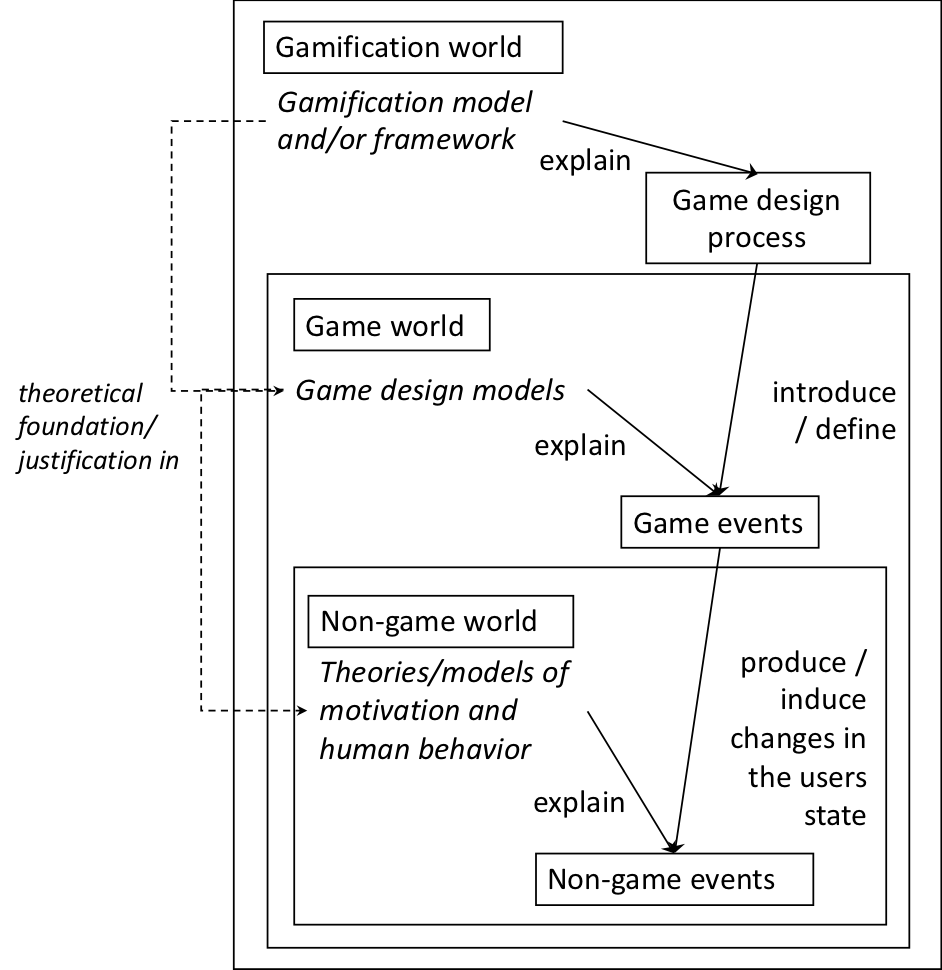
\includegraphics[width=0.55\textwidth]{images/chap-ontogacles2/nested-structure-game-nongame-worlds.png}
 \fautor
\end{figure}

Employing the nested-structure of non-game world, game world and gamification world (\autoref{fig:nested-structure-game-nongame-worlds}), the concepts in the ontology OntoGaCLeS related to the game events and non-game events have been classified in the \aspas{\emph{is-a}} hierarchy structure of class shown in \autoref{fig:is-a-hierarchy-structure-of-classes}. This structure categorizes any concept of ontology as a sub-type of classes: \emph{Gamification world}, \emph{Game world}, Non-game world, Common world, and Theory/Model. The classes defined under the categories of common, non-game, game and gamification worlds are concepts for things in their respective worlds, and the concepts formalized as sub-type of \emph{Theory/Model} define the theoretical foundation and justification of gamification and game design.

\emph{Gamification world} is the class of all things that depend of the gamification world to exist. In this sense, a concept is formalized as sub-type of \emph{Gamification world} whether it represents something that needs of gamification world to be described. For instance, the \emph{Gamification goal/purpose} is a concept formalized as sub-type of Gamification world to describe the goals and/or purposes of a gamification model and/or framework (e.g. \emph{avoiding dropout}, \emph{reducing weariness}). The basic concepts defined as sub-types of \emph{Gamification world} for the gamification of CL scenarios are: \emph{Gamified CL session}, \emph{Motivational strategy}  (\emph{Y<=I-mot goal}) by gamification, \emph{Player role}, and \emph{Individual gameplay strategy} (\emph{I-gameplay strategy}).

\emph{Game world} is the class of all things that depend of the game world to exist. Concepts formalized as sub-types of \emph{Game world} require only elements defined in the games to be described. The basic concept defined as sub-types of \emph{Game world} to gamify CL scenarios is: \emph{Game element}. \emph{Non-game world} is the class of all things that does not need concepts from the \emph{Gamification world} or \emph{Game world} to exist. The non-game world is divided in the sub-types: \emph{Learning world}, \emph{Instructional world}, \emph{World of cognition}, \emph{ID-ISD world}, \emph{CL world}, and \emph{World of motivation and human behavior}. Basic concepts defined as one of these world only need things from its respectively world to exist. Thus, for instance, the concepts formalized as sub-type of \emph{World of motivation and human behavior} represent things that only need elements from motivation and human behavior to exist, so that the basic concepts related to the gamification of CL scenarios formalized as sub-types of \emph{World of motivation and human behavior} are: Individual motivational goal (\emph{I-mot goal}), \emph{Motivation stage}, and \emph{Human need stage}.

\emph{Common world} is the class of anything used to represent things that require concepts of other worlds to be formalized. These concepts are common to the other worlds, and they have been taxonomically classified taking as base the classification defined in the upper-level ontology \textbf{YAMATO} – \emph{\textbf{Y}et \textbf{A}nother \textbf{M}ore \textbf{A}dvanced \textbf{T}op-level \textbf{O}ntology} \cite{Mizoguchi2010}. The basic concepts in the \emph{Common world} to represent persuasive game design are the concepts of: (i) \emph{action}, (ii) \emph{entity} (e.g. \emph{object}, \emph{agent}), (iii) \emph{state}, and (iv) \emph{event}. These concepts, their sub-types, and their ontological structures have been formalized following the formalization proposed by Galton and Mizoguchi in the article \aspas{\emph{The Water Falls but the Waterfall Does Not Fall: New Perspectives on Objects, Processes and Events}} \cite{GaltonMizoguchi2009}. According to these definitions, there is a mutual dependency between processes and entities whereby no one process (\emph{action}) can exist without an entity (\emph{agent} or \emph{object}) to enact it, and an entity is what it is as consequence of its processes. Therefore, an entity has properties knows as \emph{states} that change over time when processes are enacted by the object. An \emph{event} is then defined as integration of entities, actions, and states in a particular context to describe a fixed chunk of any process in which the participants of process are the agents and objects.

\begin{figure}[!htb]
 \caption{\aspas{\emph{is-a}} hierarchy structure of classes to represent concepts in the ontology OntoGaCLeS}
 \label{fig:is-a-hierarchy-structure-of-classes}
 \centering
 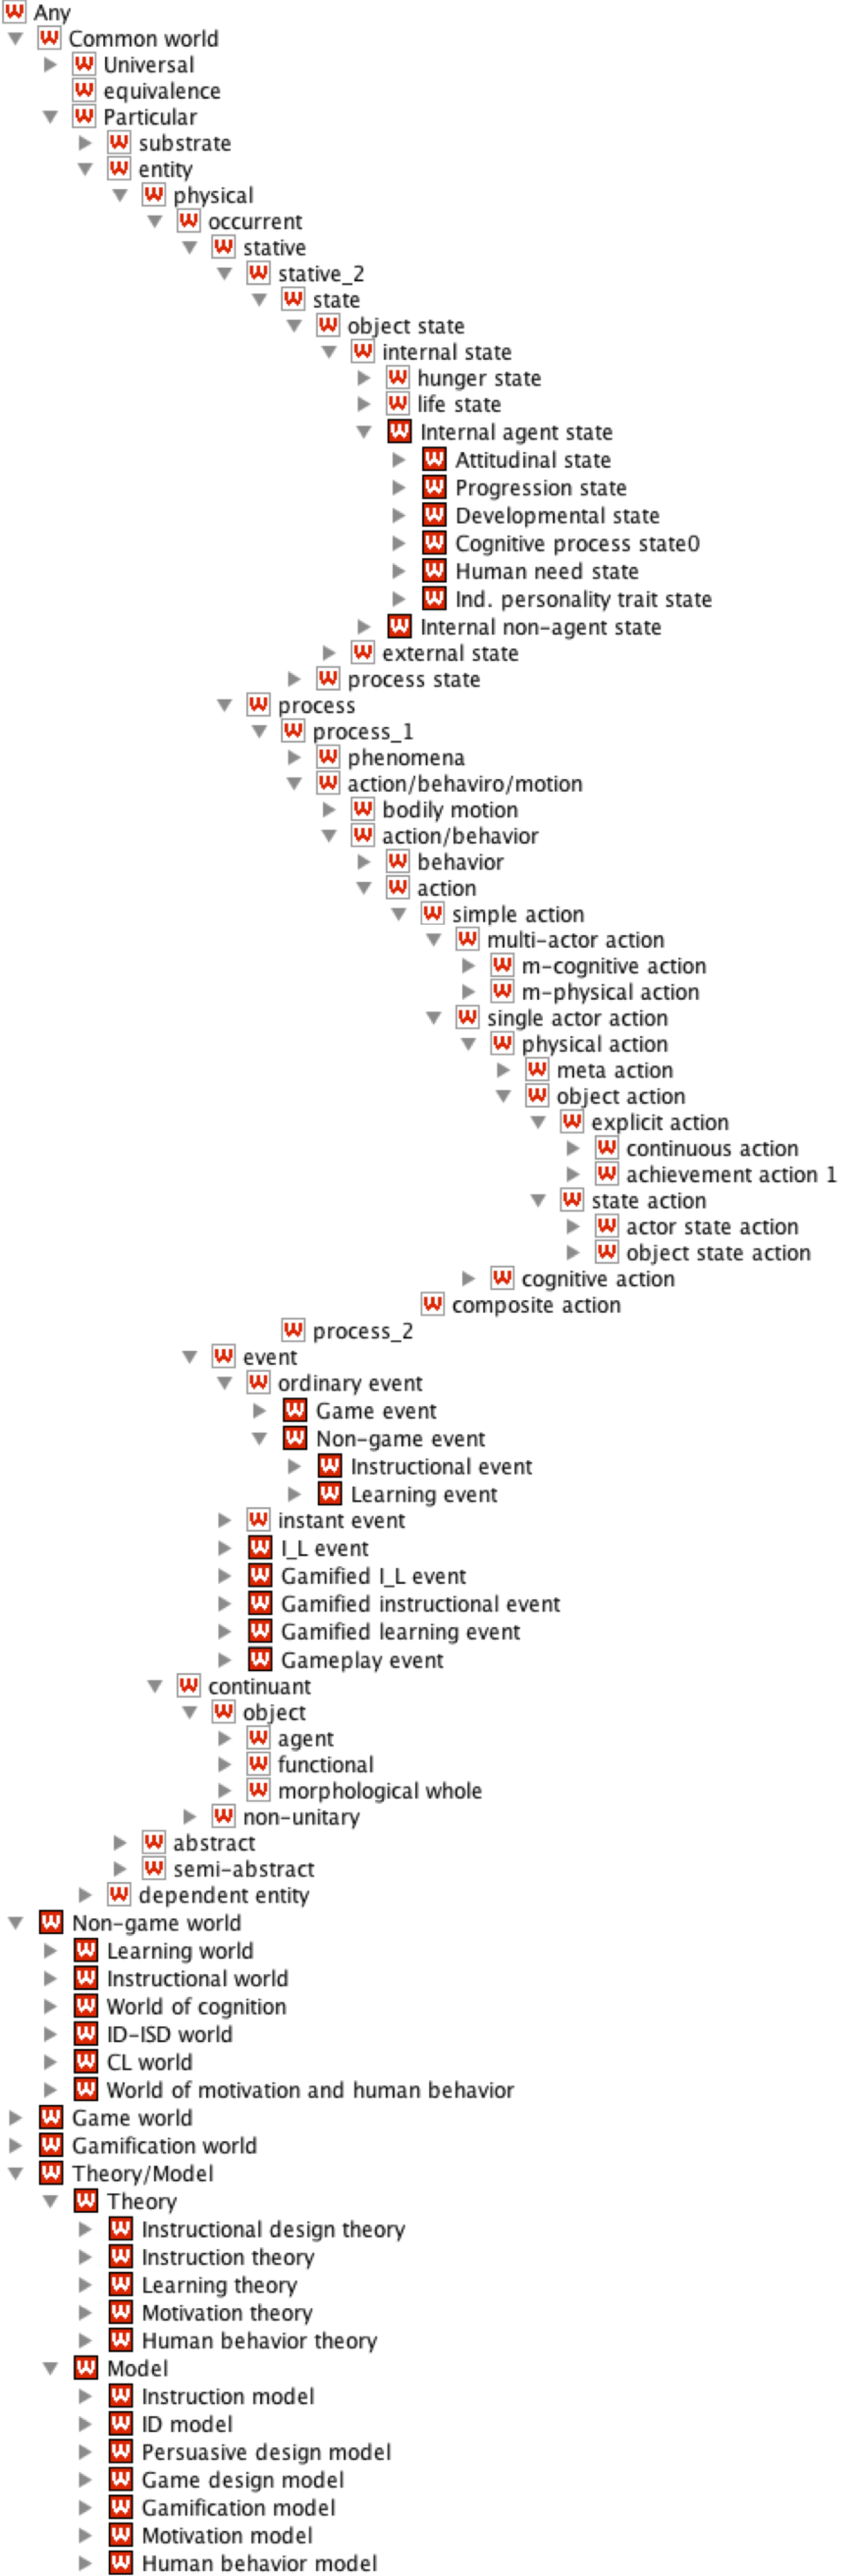
\includegraphics[width=0.46\textwidth]{images/chap-ontogacles2/is-a-hierarchy-structure-of-classes.png}
 \fautor
\end{figure}
\newpage

\autoref{fig:ontological-structures-event} shows the formalization of events as ontological structures in the ontology OntoGaCLeS. As it shown in this formalization, the class event is classified in \emph{ordinal event} and \emph{instant event} in which the ordinal event is constituted by a process (e.g. \emph{action}, \emph{behavior}), the participants in the events are entities, and the ordinal event has instantaneous events as starting and ending event to delimit the chunk of processes that compose the event. Finally, the \emph{ordinal event} is classified in \emph{Game event} and \emph{Non-game event} as shown in the \aspas{\emph{is-a}} hierarchy of classes (\autoref{fig:is-a-hierarchy-structure-of-classes}). The composed events in the \aspas{\emph{is-a}} hierarchy structure of classes are defined as subtype of \emph{event}, and they are: \emph{I\_L event}, \emph{Gameplay event}, \emph{Gamified Instructional event}, \emph{Gamified Learning event}, and \emph{Gamified I\_L event}.
The formalization as ontological structures of these events is detailed in the following sections.

\begin{figure}[!htb]
 \caption{Ontological structures to represent events}
 \label{fig:ontological-structures-event}
 \centering
 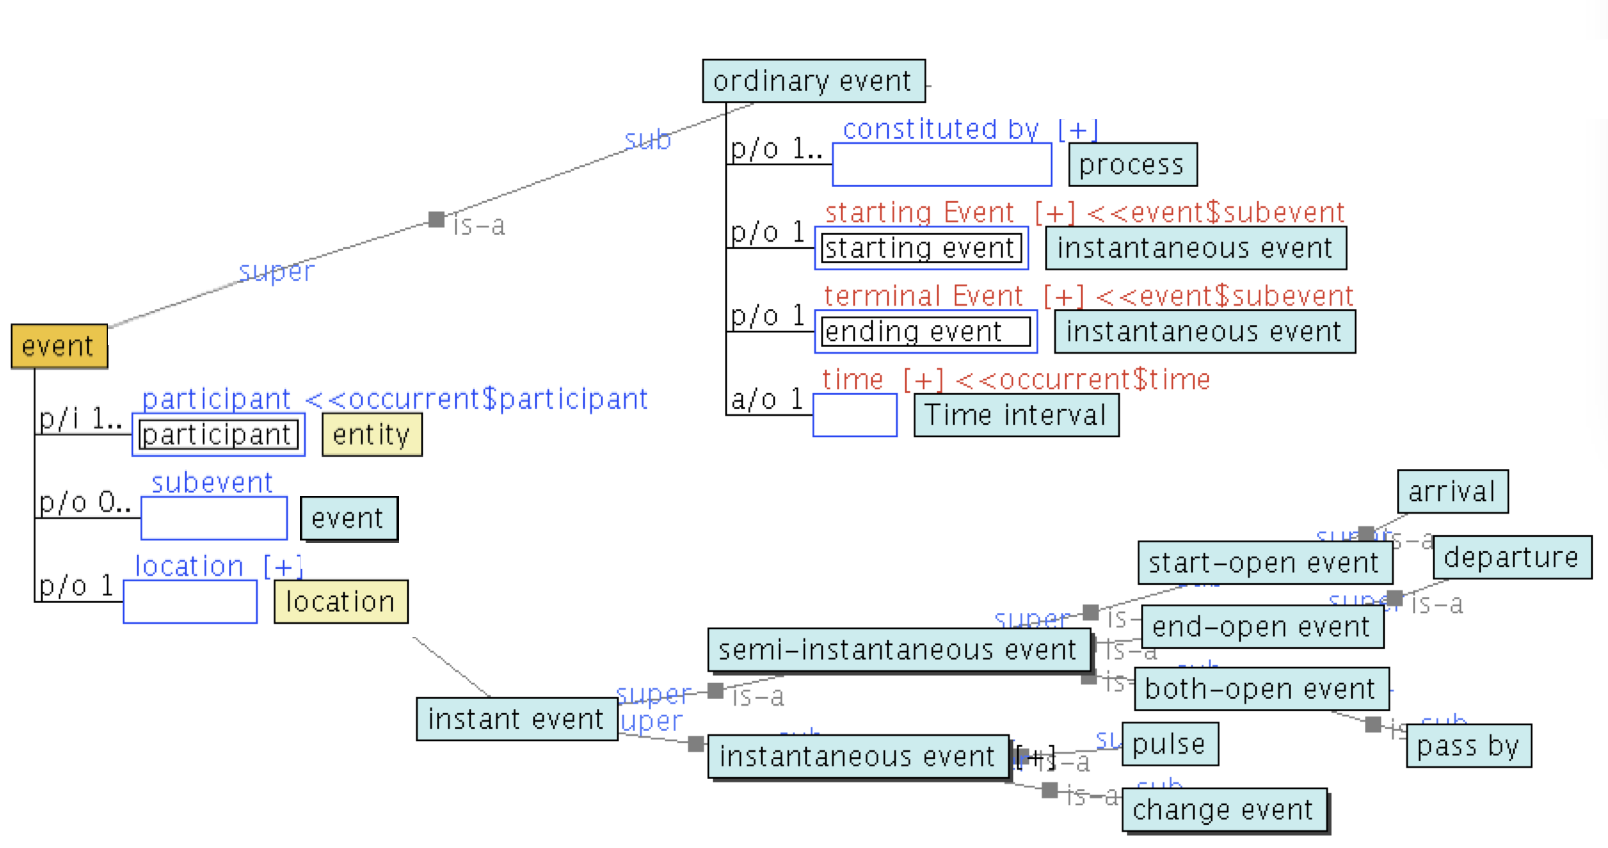
\includegraphics[width=1\textwidth]{images/chap-ontogacles2/ontological-structures-event.png}
 \fautor
\end{figure}

%%%%%%%%%%%%%%%%%%%%%%%%%%%%%%%%%%%%%%%%%%%%%%%%%%
\section[Modeling Persuasive Game Design]{Modeling Persuasive Game Design}
\label{sec:modeling-persuasive-game-design}

\emph{Persuasive Game Design} (PGD) is defined as \aspas{\emph{the game design for the purpose to change peoples’ attitudes, intentions, motivations and/or behaviors through persuasion and social influence without using coercion and/or deception}.} In this sense, to represent the PGD as ontological structures, an ontology-based formalization of the \emph{game design} is needed because PGD is conceptualized as a game design that is embedded in persuasive design.

As was explained in the previous section, game design models are used to define the game events whereby the changes in the users’ states are produced or induced in a non-game events, and these changes are explained by theories/models of motivation a human behavior. Therefore, the game design consist into establish the relation between non-game event and game event based on theoretical justification extracted from game design models and theories of motivation and human behavior. When this game design has the purpose is to change the participants' attitudes intentions, motivations, or behaviors becomes PGD, and it has been formalized in the ontology OntoGaCLeS as ontological structures to represent the \emph{persuasive gameplay event} and the \emph{WAY-knowledge of PGDS} detailed in \autoref{subsec:persuasive-gameplay-event} and \autoref{subsec:way-knowledge-of-persuasive-game-design}. Employing the ontology-based formalization of PGD, the concept of \aspas{\emph{Persuasive Gameplay Scenario Model}} has been proposed to represent the design rationale of how to apply PGD in non-game events. The formalization of this model as ontological structures is presented in \autoref{subsec:persuasive-gameplay-scenario-model}.

\subsection{Persuasive Gameplay Events}
\label{subsec:persuasive-gameplay-event}

The PGD is explicitly represented as the relation between game events and non-game events in the ontology OntoGaCLeS under the concept of \emph{Gameplay event}. This concept describes, in an explicit way, what happens in the non-game world and the game world when the user is persuaded and/or social influenced to interacts with the system. %Thus, a \emph{Persuasive gameplay event} is formalized as a explicit description of the relation between game events and a non-game event in which the doer of the non-game event has been persuaded and/or social influenced by the game events.
\autoref{fig:ontological-structures-persuasive-gameplay-events} shows the ontological structures proposed to represent persuasive gameplay events, where the \emph{Gameplay event} (at the top of figure) represents any interaction that would occur between the participants and the game elements in the system that is being gamified. In the formalization of gameplay event, the \emph{Game event} describes actions performed by an \emph{agent} that becomes \emph{Game agent}, an \emph{action} of this agent becomes \emph{Game action}, the \emph{participant} who interacts with the game agent becomes \emph{Player}, and the object produced as consequence of \emph{Game action} becomes a \emph{Game component}.

\begin{figure}[!htb]
 \caption[Ontological structures to represent persuasive gameplay events]{Ontological structures to represent persuasive gameplay events. \aspas{\emph{Gameplay event}} at the top, \aspas{\emph{Gameplay-stimulus event}} at the bottom-left, \aspas{\emph{Gameplay-mechanism event}} at the bottom-center, and \aspas{\emph{Gameplay-consequence event}} at the bottom-right.}
 \label{fig:ontological-structures-persuasive-gameplay-events}
 \centering
 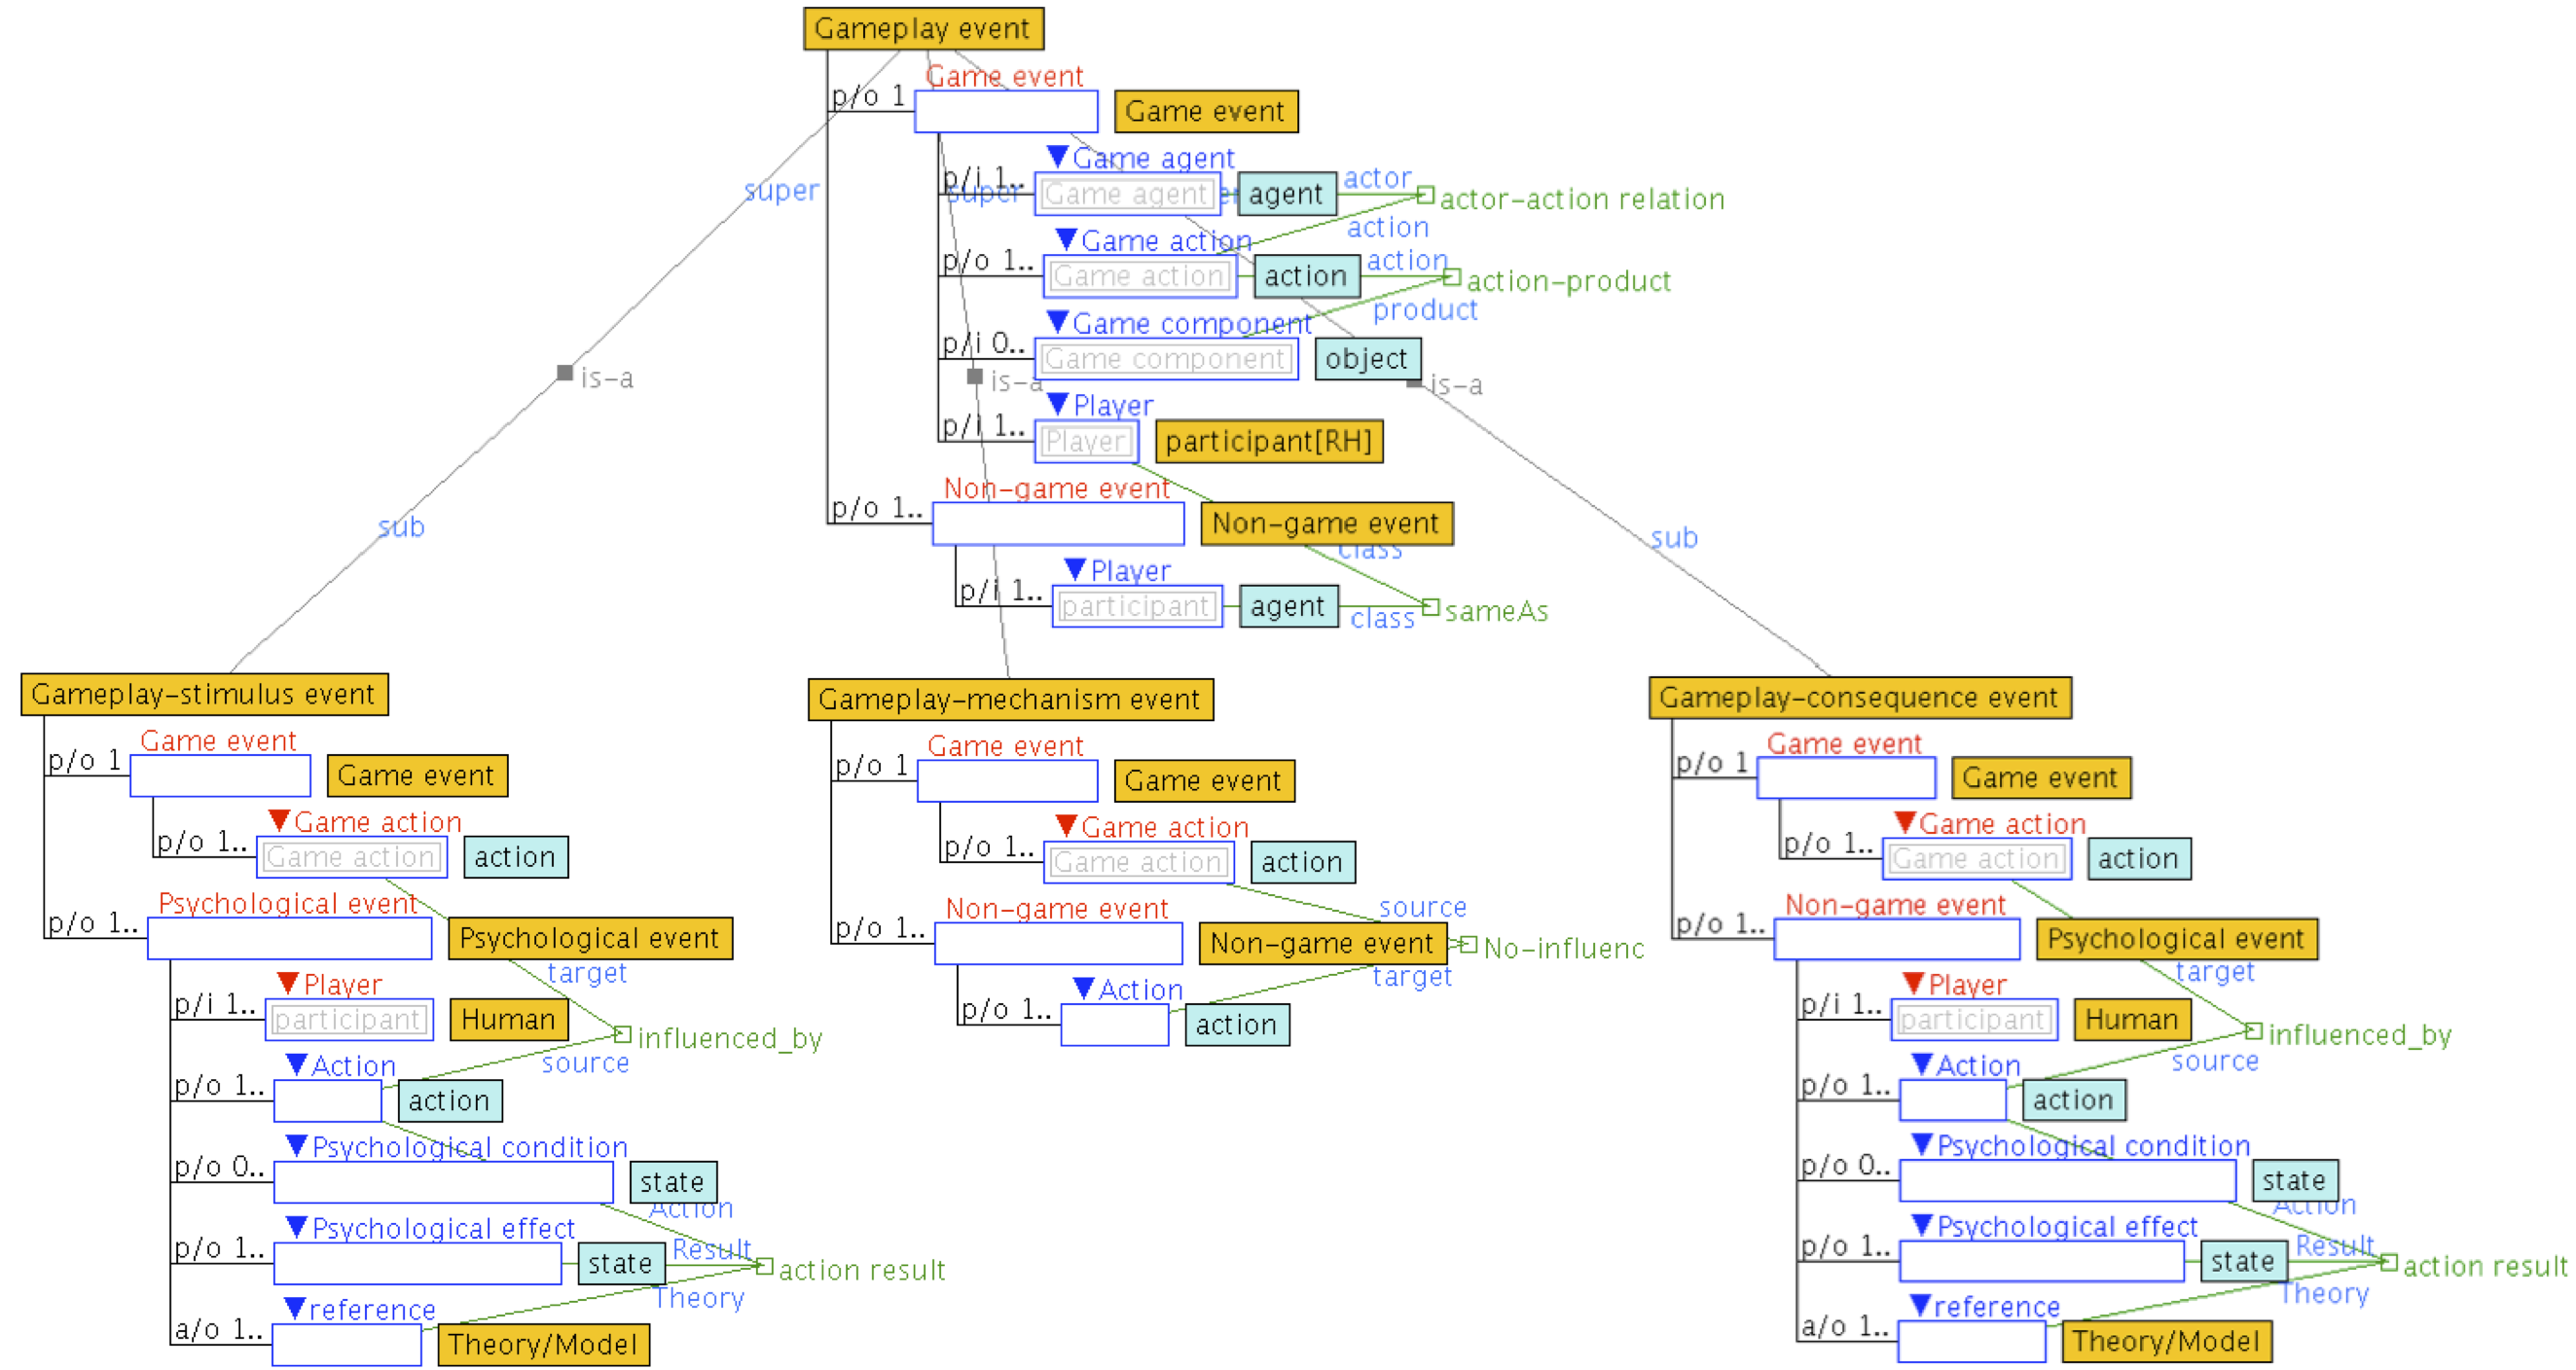
\includegraphics[width=1\textwidth]{images/chap-ontogacles2/ontological-structures-persuasive-gameplay-events.png}
 \fautor
\end{figure}

When game events are used to lead the participants into take actions by persuasion and/or social influence, there are three types of interactions defined as persuasive game events. These events are: \emph{Gameplay-stimulus event}, \emph{Gameplay-mechanism event}, and \emph{Gameplay-consequence event}. The gameplay-stimulus and gameplay-consequence events are used to represent internal psychological processes that occur by influence of a game action, whereas the gameplay-mechanism event has been formalized to represent actions that occur in the non-game world. In a \emph{Gameplay-stimulus event}, the game actions occur before the actions being gamified, and, in a \emph{Gameplay-consequence event}, the game actions occur after the actions being gamified. These both gameplay events are formalized as ontological structures shown at the bottom-left and bottom-right of \autoref{fig:ontological-structures-persuasive-gameplay-events}, where the internal psychological process associated to game actions is represented as a pair of events: \emph{Game event} and \emph{Psychological event}.
In these formalizations, the \emph{action} of the \emph{Psychological event} is \emph{influenced by} the action defined as \emph{Game action} in the \emph{Game event}. Concepts of \emph{state} are used in the psychological event to represent \emph{Psychological condition} and \emph{Psychological effect} related to the participants' changes of attitudes, intentions, motivations and/or behaviors. These changes, in the ontological structures, are explained by theories and models of motivation and human behavior (\emph{Theory/Model}) derived and/or related to persuasion and social influence, such as classical conditioning \cite{GormezanoProkasyThompsonThompson1987}, operant conditioning \cite{Skinner1953}, and Fogg's behavior model \cite{Fogg2009}.

To illustrate the use of the ontological structures presented in \autoref{fig:ontological-structures-persuasive-gameplay-events}, let us formally represent the gameplay events that occur when \aspas{\emph{a participant is persuaded to obtain points by making a comment in a post}} illustrated as a storyboard shown at the top of \autoref{fig:ontological-structures-example-persuasive-gameplay-events}. This storyboard as ontological structures is formalized at the bottom of \autoref{fig:ontological-structures-example-persuasive-gameplay-events}, where \emph{Raising motivation by promising points event} is represented as gameplay-stimulus event, the \emph{Comment post event} is represented as gameplay-mechanism event, and the \emph{Increasing behavior by giving points event} is represented as gameplay-consequence event. The game action \aspas{\emph{Promise points}} and the internal psychological process \aspas{\emph{Raise motivation}} are represented as the game-stimulus event \aspas{\emph{Raising motivation by promising points event}} shown at the left of figure. According to this structure, the psychological effect is being \emph{Motivated}, and the condition to achieve this state is being \emph{Not motivated}. This change of state is explained by the Foog's behavior model \cite{Fogg2009}. The game-mechanism event with the \emph{Comment post event} as the non-game event being gamified is shown at the center of figure, and it describes the action of \emph{Comment post} performed by the participant in a non-game system. The \emph{Increasing behavior by giving points event} at the right of figure is a gameplay-consequence event in which the action \aspas{\emph{Increase self-behavior}} is \emph{influenced by} the game action \aspas{\emph{Give points}} performed by a \emph{Point system}. The Foog's behavior grid model explains the change described in the psychological event in which the psychological condition is \emph{Being non-familiar behavior} and the psychological effect is \emph{Being familiar behavior}.

\begin{figure}[!htb]
 \caption[Example of ontological structures to represent persuasive gameplay events]{Example of ontological structures to represent persuasive gameplay events in which  \aspas{\emph{a participant is persuaded to obtain points by making a comment in a post}} (at the bottom). At the top, the storyboard of gameplay events involved in this example.}
 \label{fig:ontological-structures-example-persuasive-gameplay-events}
 \centering
 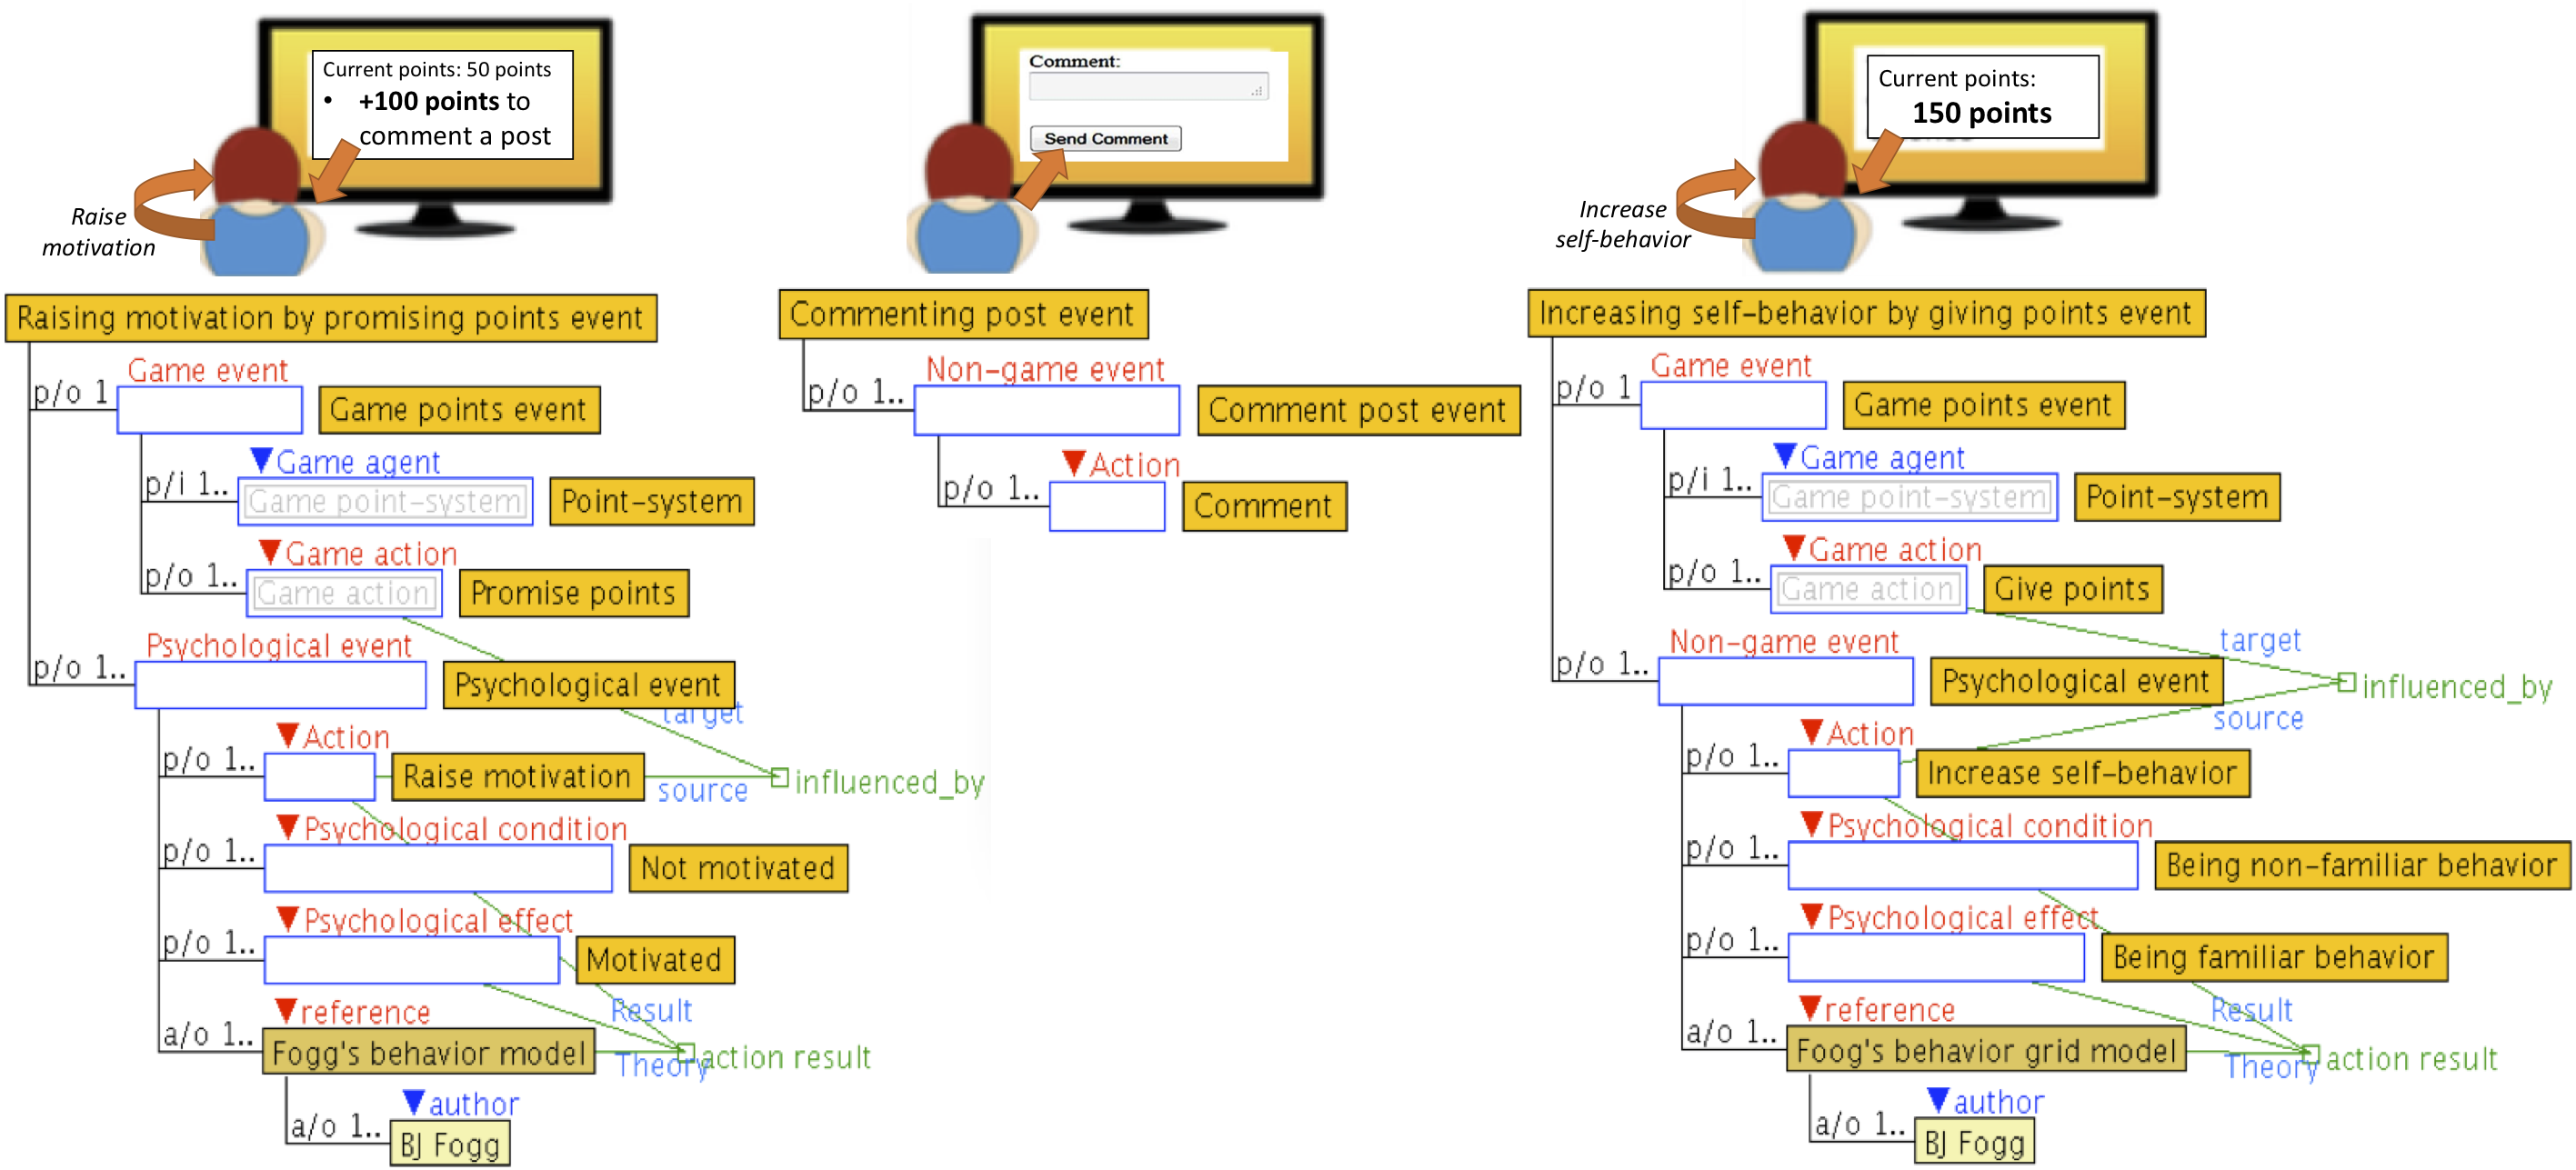
\includegraphics[width=1\textwidth]{images/chap-ontogacles2/ontological-structures-example-persuasive-gameplay-events.png}
 \fautor
\end{figure}

\subsection{WAY-knowledge of PGDS}
\label{subsec:way-knowledge-of-persuasive-game-design}

\emph{WAY-knowledge of PGDS} is a prescriptive description of PGD in which the relation between game events and non-game events is defined as a decomposition method of gameplay events. Thus, to describe how to achieve a specific change in the participants' attitudes and attitudes, intentions, motivations and/or behaviors, a gameplay event can be broken down into several gameplay-event sequences. The strategy of choosing a decomposition method to be applied in gameplay-event are know as \emph{Game Design Strategy} (GDS), and when it is performed according to persuasive principles, it is known as \emph{Persuasive Game Design Strategy} (PGDS).

PGDSs are game design strategies that are embedded in persuasive strategies, and their representation as \emph{WAY-knowledge} constitutes a game design with the dedicate function to persuade and/or to cause social influence in the participants of non-game events. Therefore, the formalization of the knowledge involved in the PGDSs has been defined in the ontology OntoGaCLeS as a simplified version of the \emph{WAY-structure} proposed by \citeonline{KitamuraMizoguchi2004,KitamuraKashiwaseFuseMizoguchi2004} to represent functions. The simplified version of the \emph{WAY-structure} has been formalized as the ontological structure \aspas{\emph{WAY-knowledge}} shown at the top of \autoref{fig:ontological-structures-way-knowledge-of-pgds} in which the sequence of \emph{micro}-events represents the way to accomplish the \emph{macro}-event. This decomposition, known as way knowledge, is theoretical grounded in a \emph{Theory/Model} described as attribute \aspas{\emph{Theory for reference}} in the ontological structure to represent the \emph{WAY-knowledge}.

\begin{figure}[!htb]
 \caption[Ontological structures to represent \emph{WAY-knowledge of PGDS}]{Ontological structures to represent \aspas{\emph{WAY-knowledge of PGDS}.}}
 \label{fig:ontological-structures-way-knowledge-of-pgds}
 \centering
 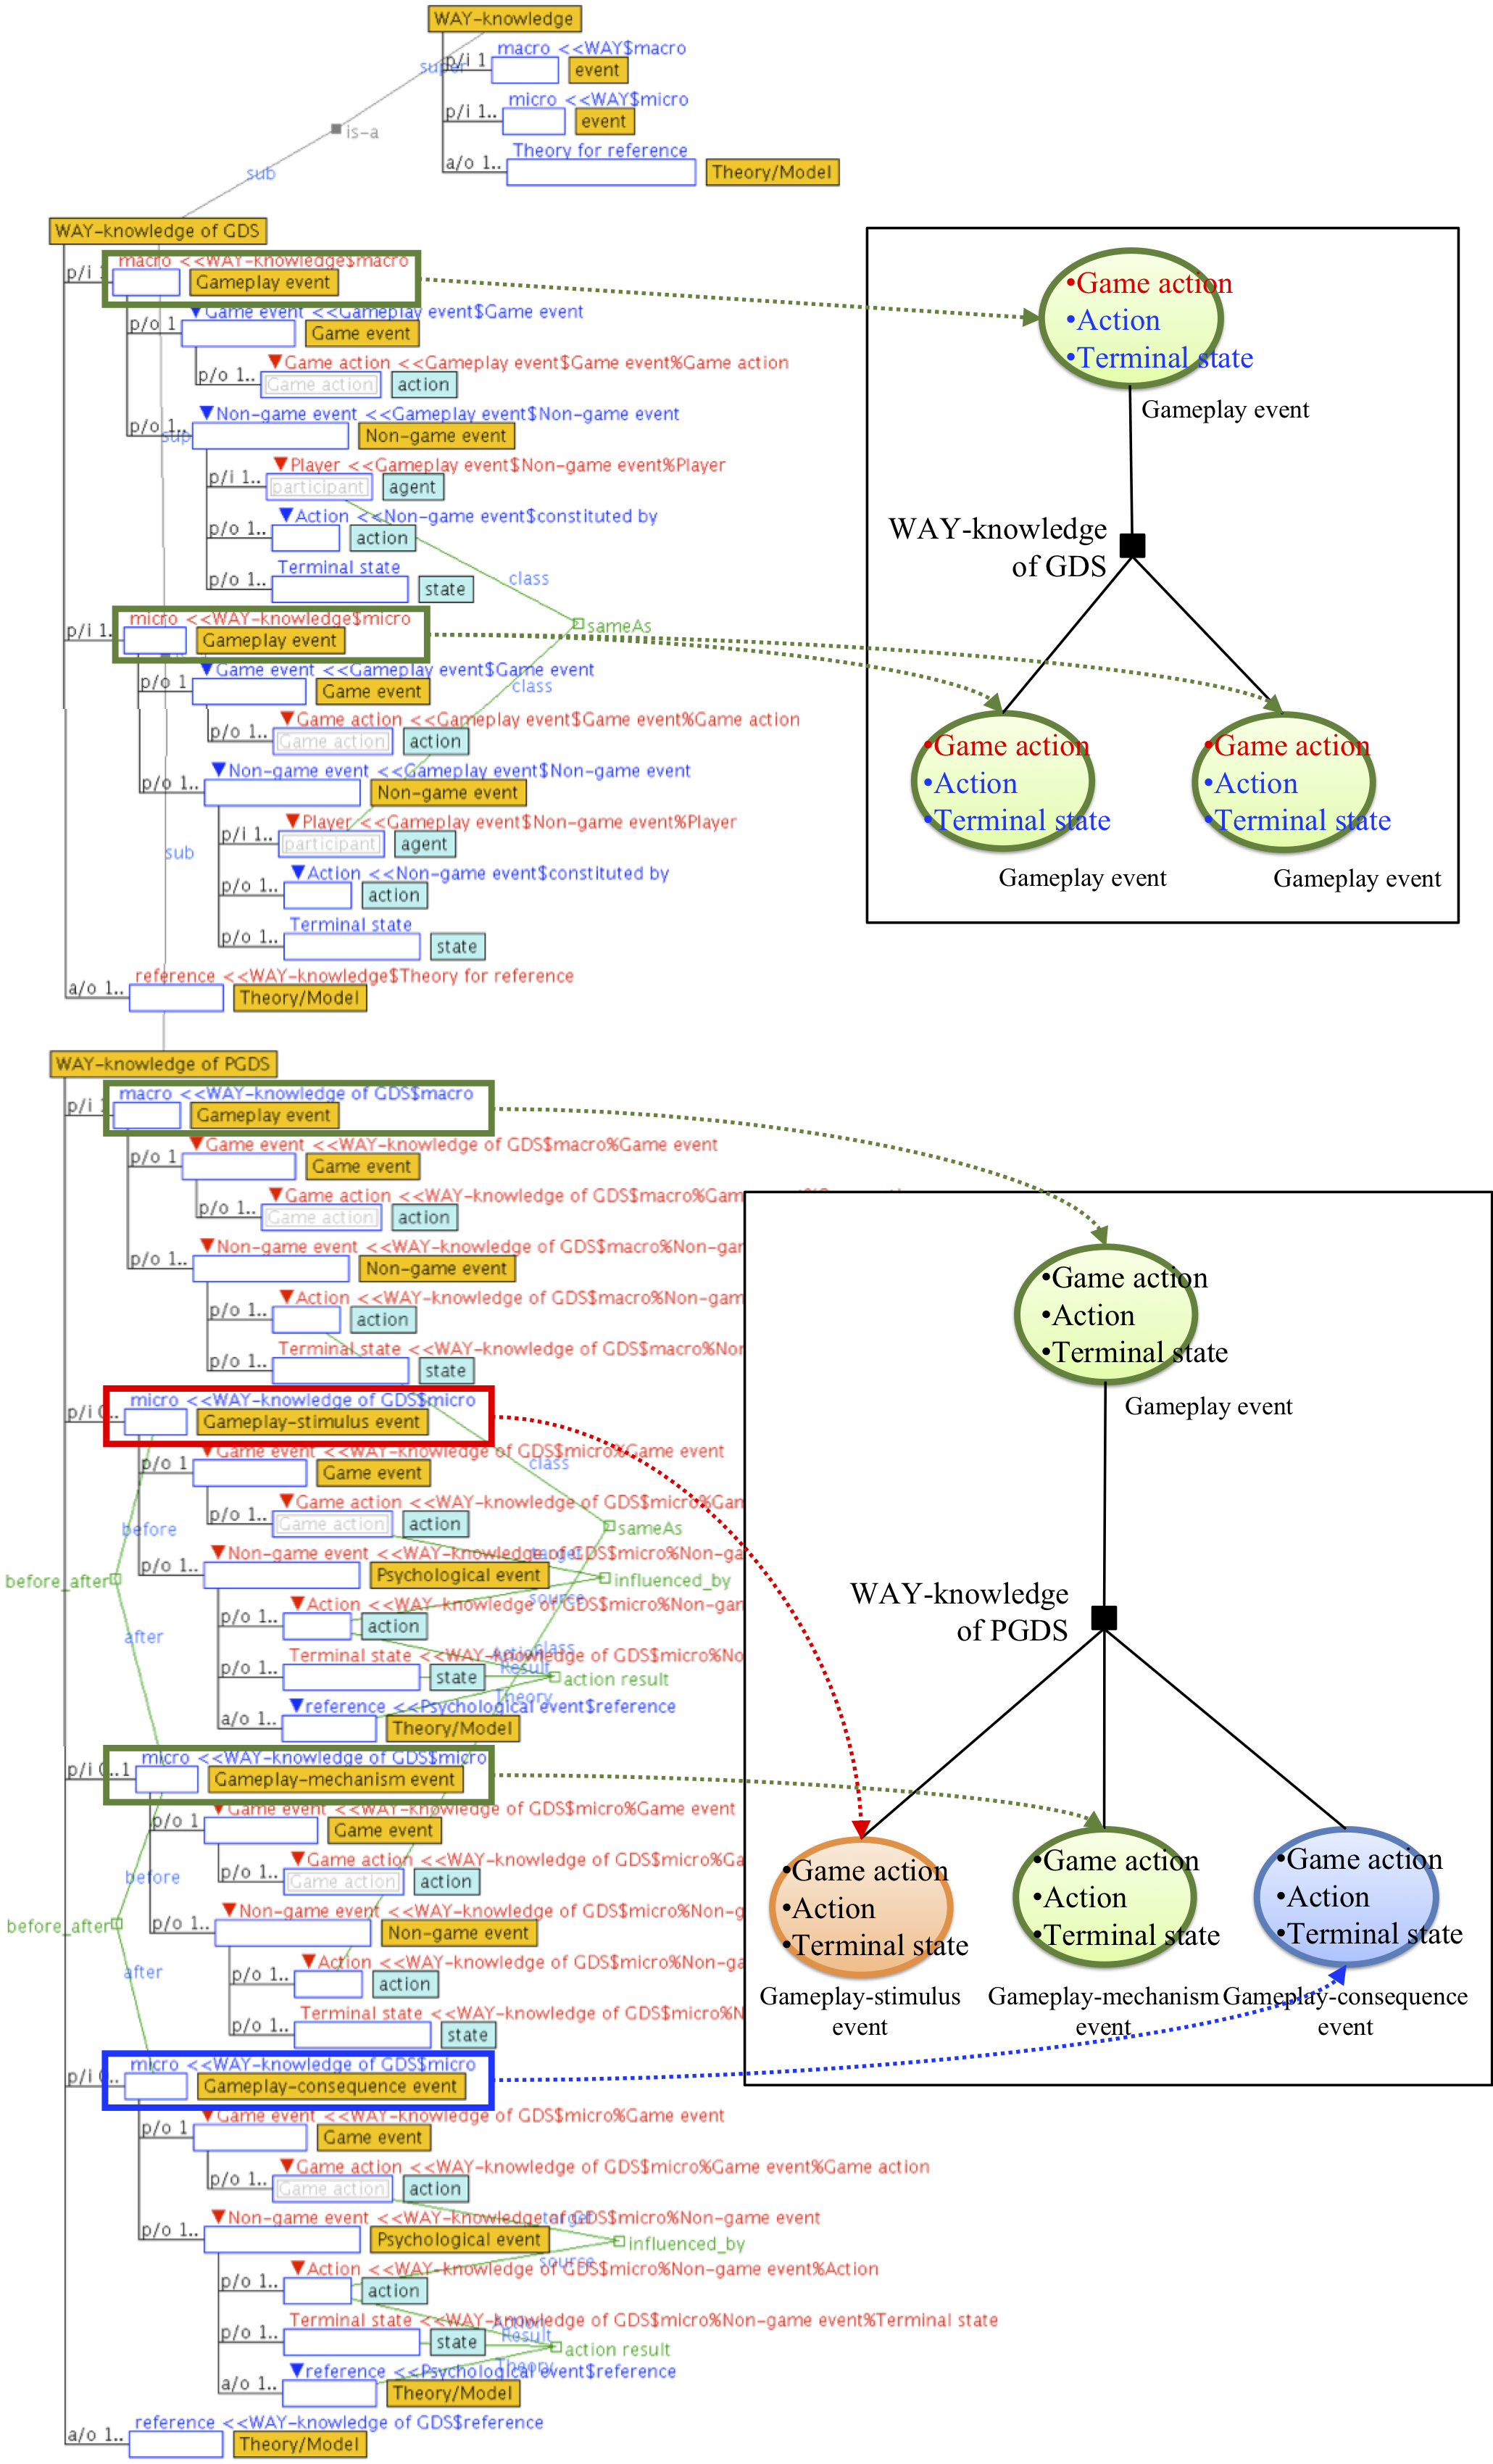
\includegraphics[width=0.84\textwidth]{images/chap-ontogacles2/ontological-structures-way-knowledge-of-pgds.png}
 \fautor
\end{figure}
\newpage

On the left side of the \autoref{fig:ontological-structures-way-knowledge-of-pgds}, the way knowledge about how to engender an expected terminal state in the player through his/her interaction with game elements is formalized as the ontological structure \aspas{\emph{WAY-knowledge of GDS}.} This ontological structure is a prescriptive description of the game design in which the decomposition tree shown at the right side of the figure indicates that the \emph{Terminal state} in the \emph{macro}-gameplay event is achieved by a sequence of \emph{micro}-gameplay events. The way knowledge about how to achieve expected change in participants' attitudes, intentions, motivations and/or behaviors through interaction with the game elements is represented as the ontological structure \aspas{\emph{WAY-knowledge of PGDS}} shown on the left side of the figure. This structure represents the relation between game events and non-game events as the decomposition method of a \emph{macro}-gameplay event into a sequence of \emph{Gameplay-stimulus events}, \emph{Gameplay-mechanism events} and \emph{Gameplay-consequence events} as shown in the decomposition tree shown on the right side of the figure. According to this ontological structure, the \emph{Terminal state} in the \emph{macro}-gameplay event represents \aspas{\emph{what to achieve}} as the goal of decomposition method, and the terminal states in the \emph{micro}-gameplay events represent \aspas{\emph{how to achieve}} this goal as a sequence of sub-goals to be achieved by the \emph{micro}-gameplay events. The goals and sub-goals as terminal states are result of actions performed by the participants in the non-game events, and when these actions are part of a internal psychological process (e.g raising motivation, increase self-behavior) influenced by game actions defined in the game events, the \emph{micro}-gameplay event is a \aspas{\emph{Gameplay-stimulus event}} or a \aspas{\emph{Gameplay-consequence event}.} The decomposition method is theoretically justified on \emph{Theory/Model} that are \emph{reference} as an \emph{attribute-of} in the ontological structure to represent \aspas{\emph{WAY-knowledge of PGDS}.}

Based on the ontological structures to represent \aspas{\emph{WAY-knowledge of PGDS}} (\autoref{fig:ontological-structures-way-knowledge-of-pgds}), a WAY-knowledge base of GDSs and PGDSs has been defined in the ontology OntoGaCLeS. Part of this base is shown in \autoref{fig:portion-way-knowledge-base-pgds}, where the PGDSs were formalized based on the Persuasive System Design (PSD) proposed by \citeonline{Oinas-KukkonenHarjumaa2009}. These PGDSs were firstly classified according to the categories of persuasive principles, and secondly, according to the expected changes in the participants' states. The decomposition tree of two PGDSs are shown in this figure in which the PGDS \aspas{\emph{Reward strategy to be motivated and to make familiar behavior based on PSD}} has been classified as a \emph{Reward strategy} in the \emph{PGDS for dialogue}, and the PGDS \aspas{\emph{Suggestion strategy to be attentive based on PSD}} has been classified as \emph{Suggestion strategy} in the \emph{PGDS for dialog}. The PGDS \aspas{\emph{Reward strategy to be motivated and to make familiar behavior based on PSD}} decomposes the \emph{macro}-gameplay event into three \emph{micro}-gameplay events defined by the game actions: \emph{Promise reward}, \emph{Await}, and \emph{Give reward}. During the gameplay-stimulus event defined by the game action \aspas{\emph{Promise reward},} the internal psychological process is \emph{Raise motivation} to achieve the \emph{Terminal state} \aspas{being \emph{Motivated}.} For the gameplay-consequence event defined by the game action \aspas{\emph{Give reward},} the internal psychological process is \emph{Increase self-behavior} to achieve the \emph{Terminal state} \aspas{\emph{Being familiar behavior}.} The decomposition tree of the PGDS \aspas{\emph{Suggestion strategy to be attentive based on PSD}} indicates that, to achieve the \emph{Terminal state} of \emph{Being attentive}, it is necessary to follow the sequence of two \emph{micro}-gameplay events defined by the game actions \aspas{\emph{Give suggestion}} and \aspas{\emph{Await}.} The internal psychological process \aspas{\emph{Focus attention}} in the gameplay-stimulus even is influenced by the game action \aspas{\emph{Give suggestion}} achieving the \emph{Terminal state} \aspas{\emph{Being attentive}.}

\begin{figure}[!htb]
 \caption{A portion of the WAY-knowledge base of game design strategies and persuasive game design strategies defined in the ontology OntoGaCLeS}
 \label{fig:portion-way-knowledge-base-pgds}
 \centering
 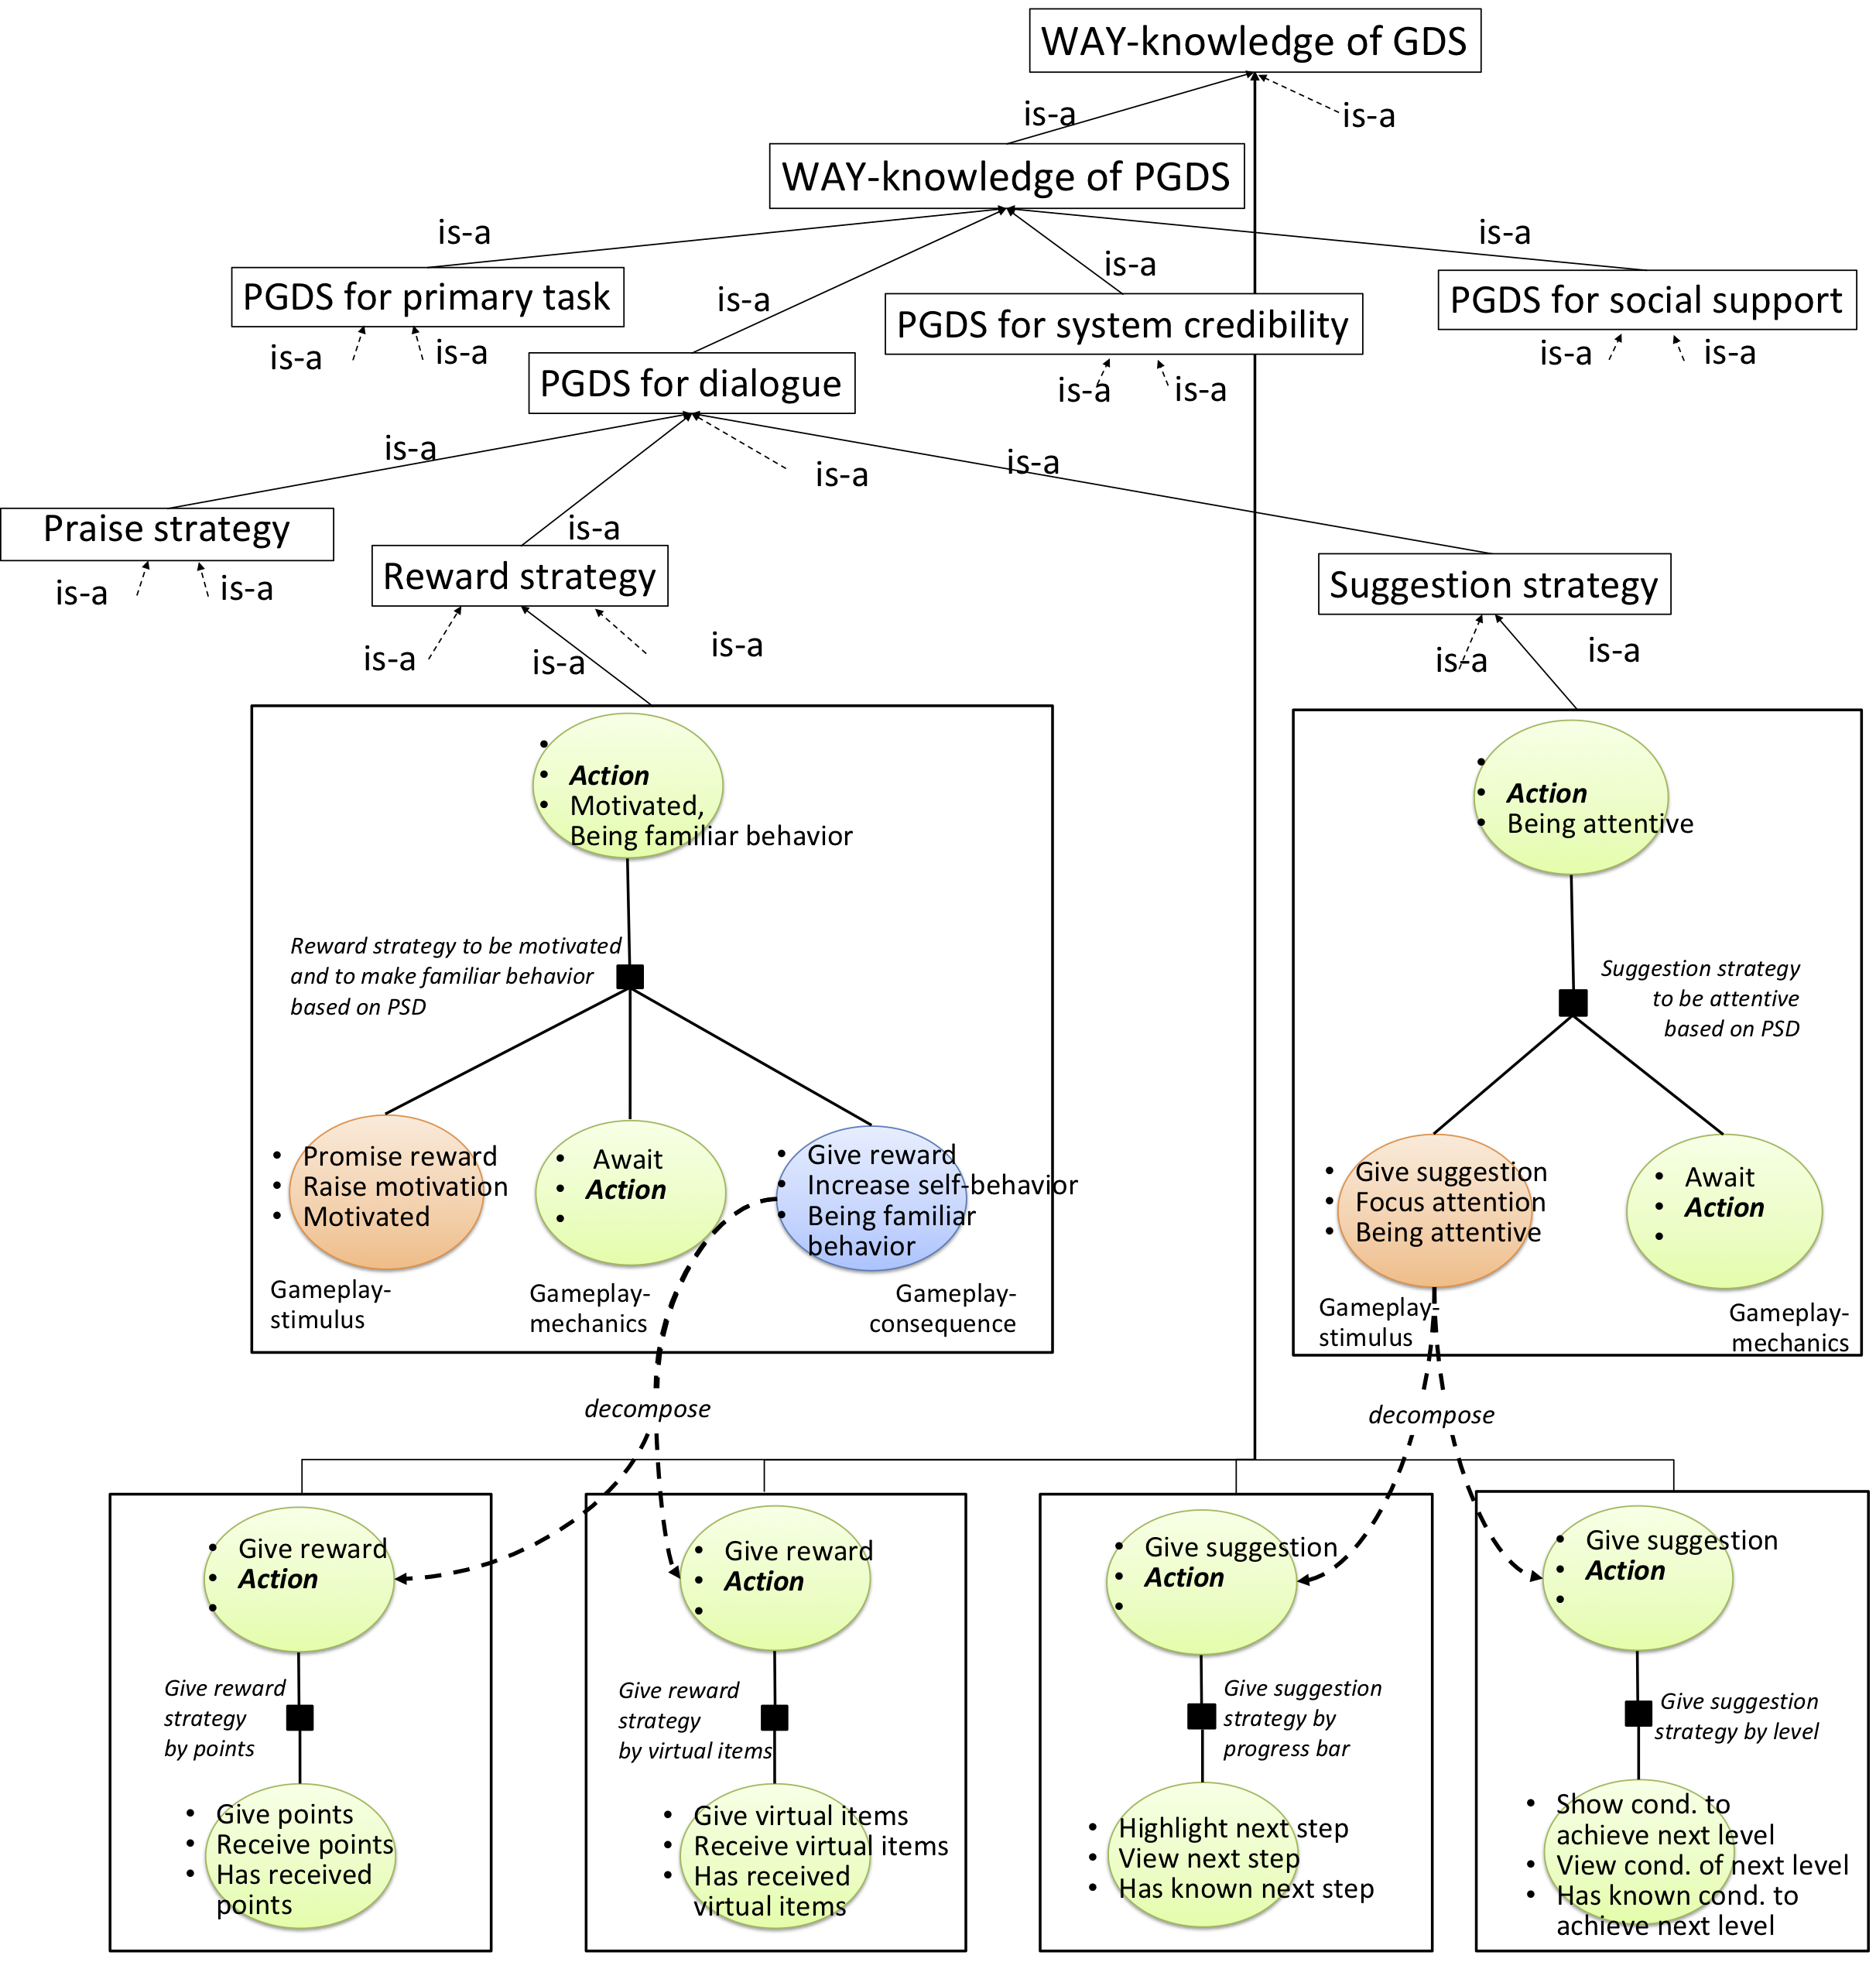
\includegraphics[width=1\textwidth]{images/chap-ontogacles2/portion-way-knowledge-base-pgds.png}
 \fautor
\end{figure}

\autoref{fig:portion-way-knowledge-base-pgds} also shows the decomposition tree of four GDSs that has been formalized based on the information extracted from the Model-driven persuasive game proposed by \citeonline{Orji2014}. The former two, known as \aspas{\emph{Give reward strategy by points}} and \aspas{\emph{Give reward strategy by virtual items},} are GDSs in which the game actions \aspas{\emph{Give points}} and \aspas{\emph{Give virtual items}} cause the \emph{Terminal state} \aspas{\emph{Has received points}} and \aspas{\emph{Has received virtual items}} by the actions \aspas{\emph{Receive points}} and \aspas{\emph{Receive virtual item}.} The latter two GDSs are \aspas{\emph{Give suggestion strategy by progress bar}} and \aspas{\emph{Give suggestion strategy by level}} to achieve the \emph{Terminal state}  \aspas{\emph{Has known next step}} and \aspas{\emph{Has known cond. to achieve next level}} by the actions \aspas{\emph{View next step}} and \aspas{\emph{View cond. of next level}.}

The ontological structure to represent the PGDS \aspas{\emph{Reward strategy to be motivated and to make familiar behavior based on PSD}} is shown in \autoref{fig:ontological-structure-reward-strategy-psd}, where the \emph{Terminal state} as goal of the decomposition tree is defined as \emph{Being attentive} in the \emph{macro}-gameplay event.
The sequence of \emph{micro}-gameplay events defined by this PGDS is defined as a gameplay-stimulus event with the game action \aspas{\emph{Give suggestion},} and a gameplay-mechanism event with the game action \aspas{\emph{Await}.} The terminal state in the gameplay-consequence event is \emph{Being attentive} achieved by the internal psychological process \aspas{\emph{Focus attention}} \emph{influenced by} the game action \aspas{\emph{Give suggestion}.} This psychological effect has theoretical justification in the ARCS model \cite{Keller1987} indicated in the attribute of \emph{reference} in the \emph{Psychological event} of the \emph{Gameplay-stimulus event}.

\begin{figure}[!htb]
 \caption[Ontological structure to represent the \emph{Suggestion strategy to be attentive based on PSD}]{Ontological structure to represent the \aspas{\emph{Suggestion strategy to be attentive based on PSD}}}
 \label{fig:ontological-structure-reward-strategy-psd}
 \centering
 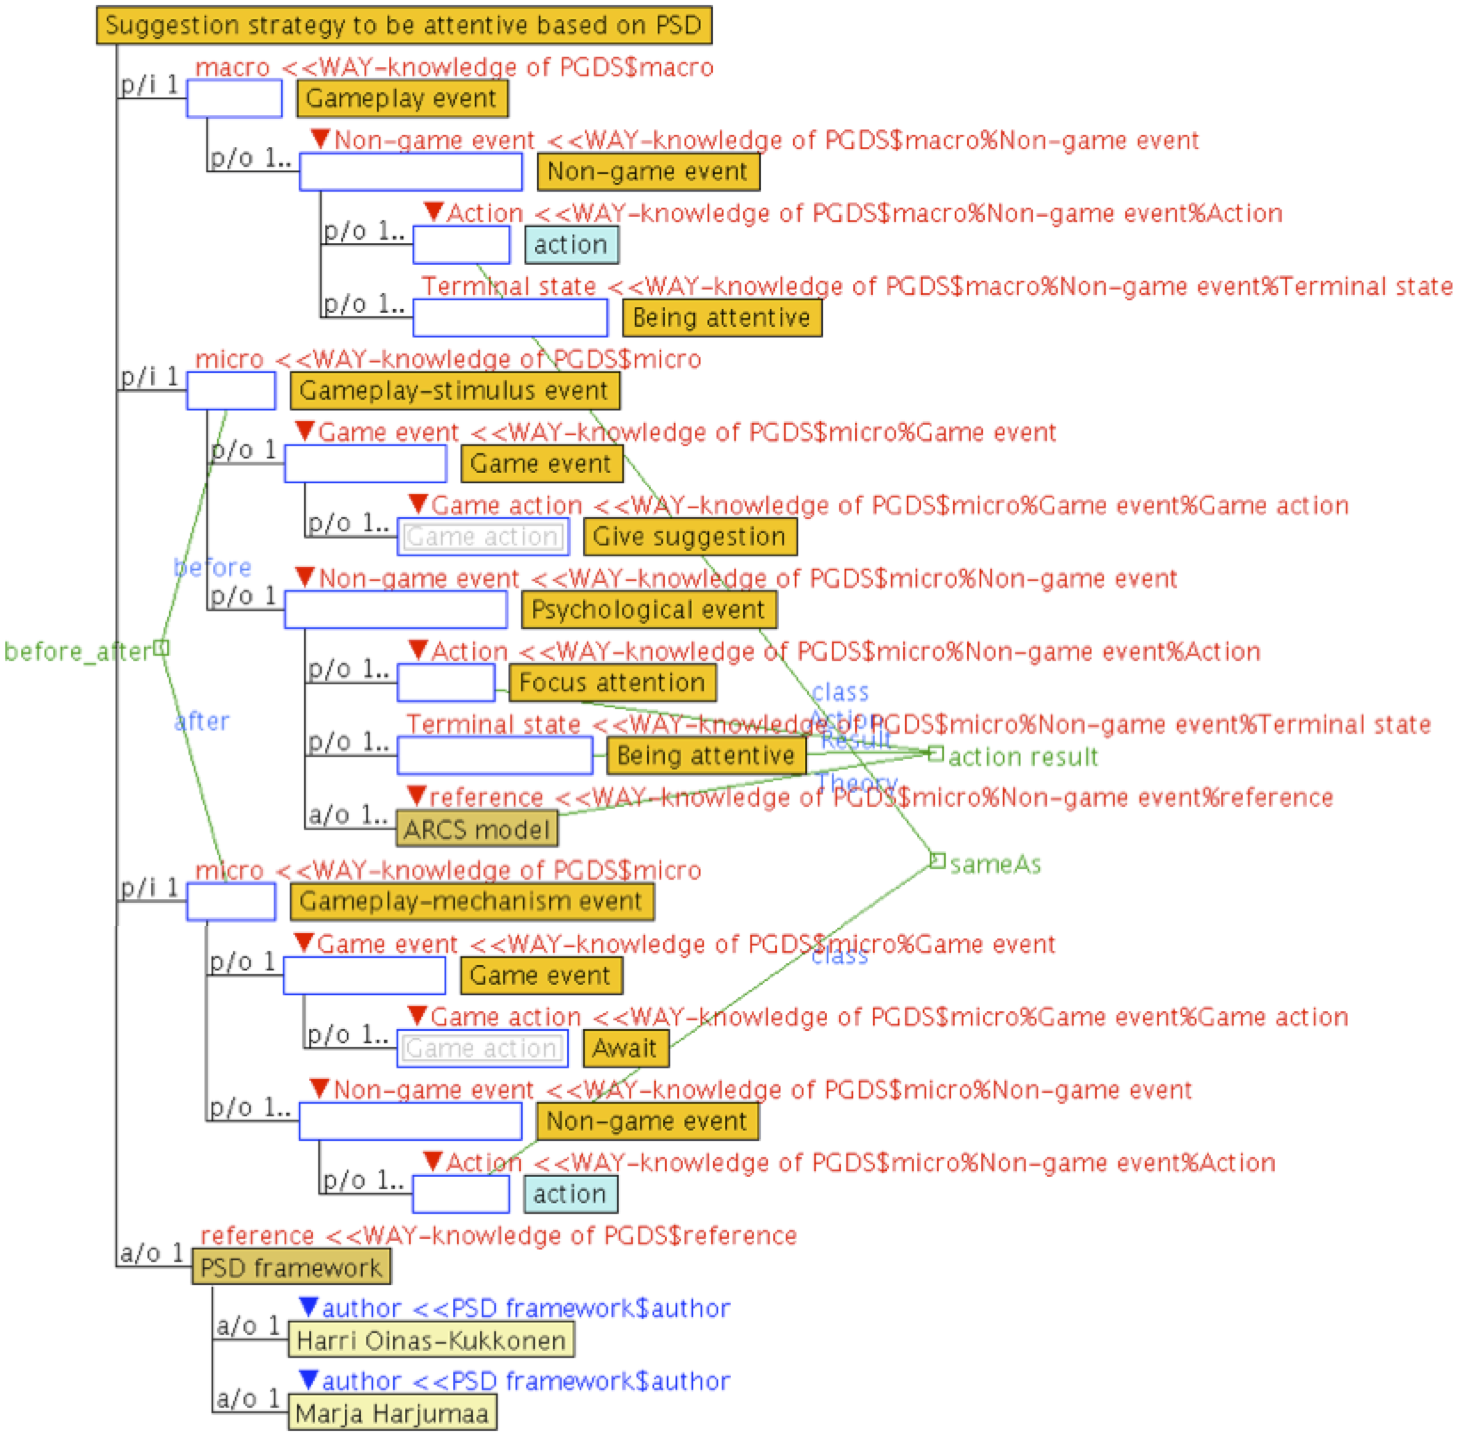
\includegraphics[width=0.9\textwidth]{images/chap-ontogacles2/ontological-structure-reward-strategy-psd.png}
 \fautor
\end{figure}

\subsection{Persuasive Gameplay Scenario Model}
\label{subsec:persuasive-gameplay-scenario-model}

\aspas{\emph{Persuasive Gameplay Scenario Model}} is an abstract structure to indicate the design rationale involved in the application of PGD in non-game events. This design rationale indicates the changes in the participants' attitudes, intentions, motivations and/or behaviors, and how these changes are achieved by a sequence of gameplay-events. The persuasive gameplay scenario model is constructed by applying the PGDSs into non-game events in a phased manner obtaining a sequence of gameplay-stimulus, gameplay-mechanisms and game-consequence events. The determination of when to stop the application of PGDSs is arbitrary for the model authors, and lies outside the scope of the modeling. \autoref{fig:ontological-structure-persuasive-gameplay-scenario-model} shows the ontological structures proposed in the ontology OntoGaCLeS to represent a persuasive gameplay scenario model. In the ontological structure \aspas{\emph{Gameplay Scenario Model},} the \emph{WAY-knowledge of GDS} is represented as a link between two gameplay events playing the roles of \emph{root} and \emph{sub} to describe the \emph{macro}-gameplay event and the sequence of \emph{micro}-gameplay events resulting of the decomposition method. In the ontological structure \aspas{\emph{Persuasive Gameplay Scenario Model},} the \emph{WAY-knowledge of PGDS} is represented as a link between a \emph{macro}-gameplay event playing the role of \emph{root}, and four \emph{micro}-gameplay events playing the role of \emph{sub}. In both ontological structures, the concept of \emph{Gameplay Scenario Model} plays the role of \emph{sub} to represent the recursive application of PGDSs and GDSs in the modeling of design rationale to gamify a non-game event.

\begin{figure}[!htb]
 \caption[Ontological structures to represent a persuasive gameplay scenario model]{Ontological structures to represent a \aspas{\emph{Persuasive Gameplay Scenario Model}}}
 \label{fig:ontological-structure-persuasive-gameplay-scenario-model}
 \centering
 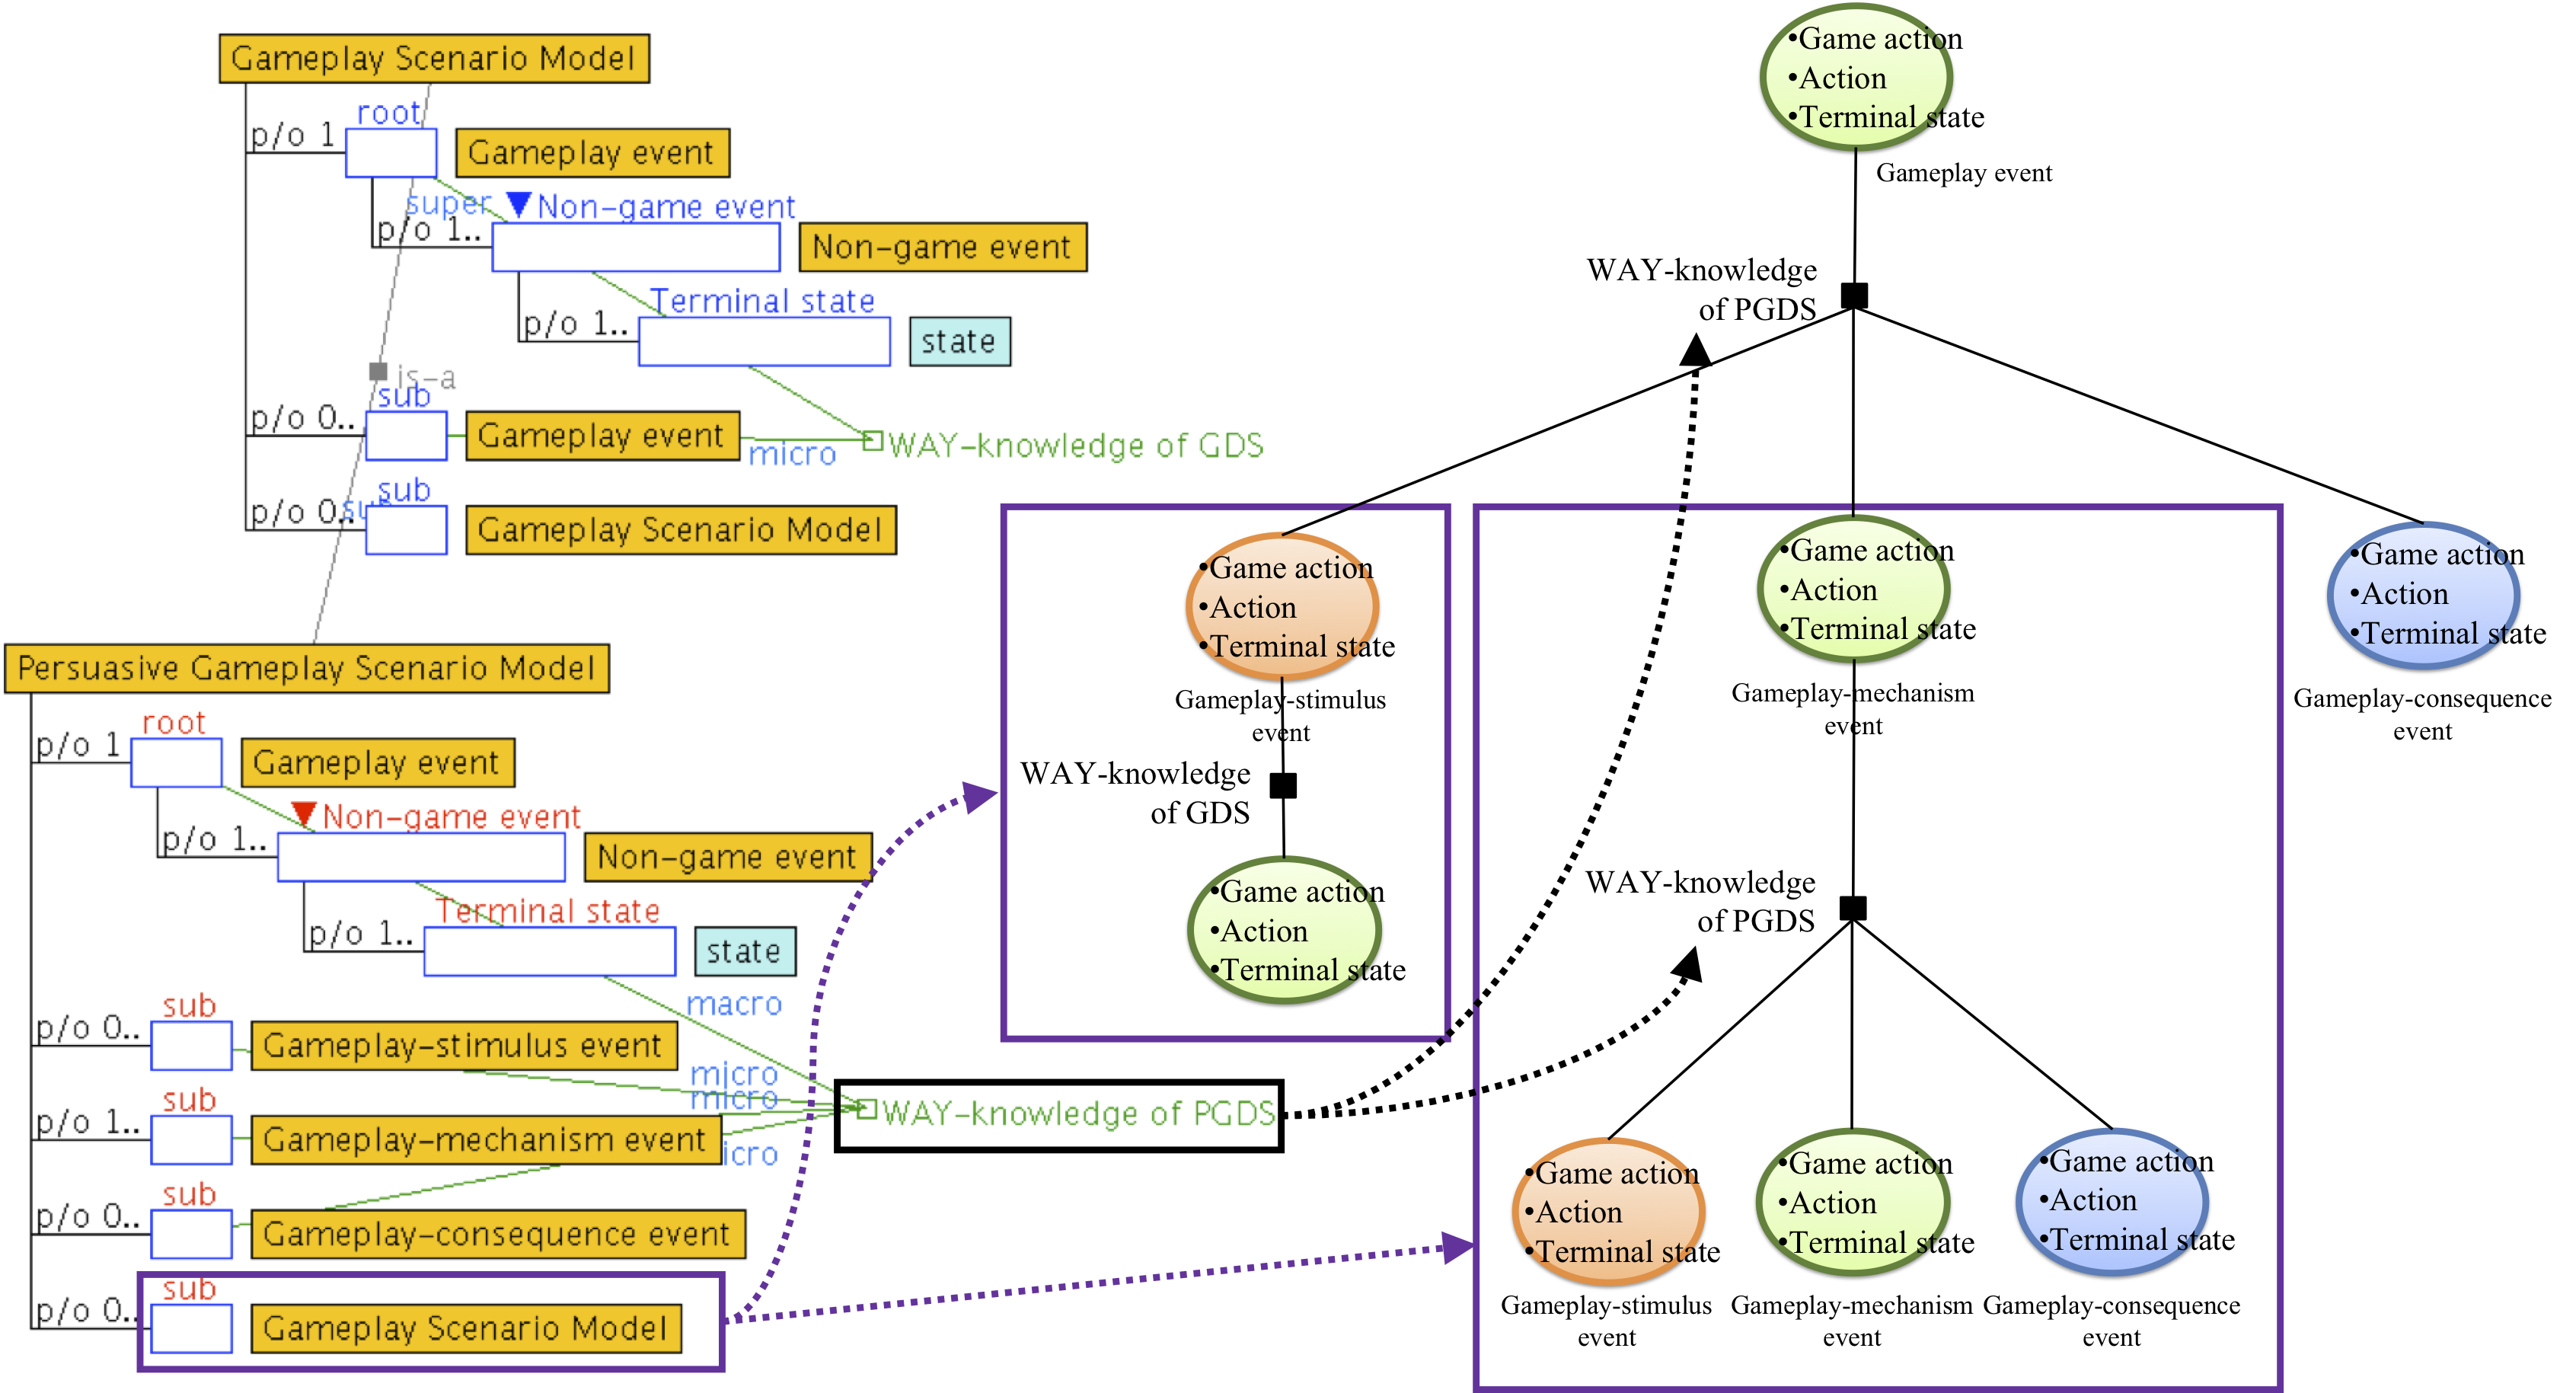
\includegraphics[width=1\textwidth]{images/chap-ontogacles2/ontological-structure-persuasive-gameplay-scenario-model.png}
 \fautor
\end{figure}

%Employing the decomposition trees presented in \autoref{fig:ontological-structure-persuasive-gameplay-scenario-model},
An example of persuasive gameplay scenario model is shown in \autoref{fig:decomposition-tree-gamified-giving-information-scenario-model}. This model represents the design rationale to gamify the instructional event \aspas{\emph{Giving information}} obtained by the application of two PGDSs and three GDSs. The PGDS \aspas{\emph{Reward strategy to be motivated and to make familiar behavior based on PDS}} has been applied to achieve the \emph{Terminal state} of \emph{Motivated} and \emph{Being familiar behavior}, and the PGDS \aspas{\emph{Suggestion strategy to be attentive based on PSD}} has been applied to achieve the \emph{Terminal state} of \emph{Being attentive}. The GDSs \aspas{\emph{Promise reward strategy by points},} \aspas{\emph{Give suggestion strategy by level},} and \aspas{\emph{Give reward strategy by points}} have been applied to accomplish the game actions \aspas{\emph{Promise reward},} \aspas{\emph{Give suggestion},} and \aspas{\emph{Give reward}} achieving the terminal states of \aspas{\emph{Has received the promise points},} \aspas{\emph{Has known cond. to achieve next level},} and \aspas{\emph{Has received points}.}

\begin{figure}[!htb]
 \caption{Example of persuasive gameplay scenario model for the gamification of \emph{Giving information}}
 \label{fig:decomposition-tree-gamified-giving-information-scenario-model}
 \centering
 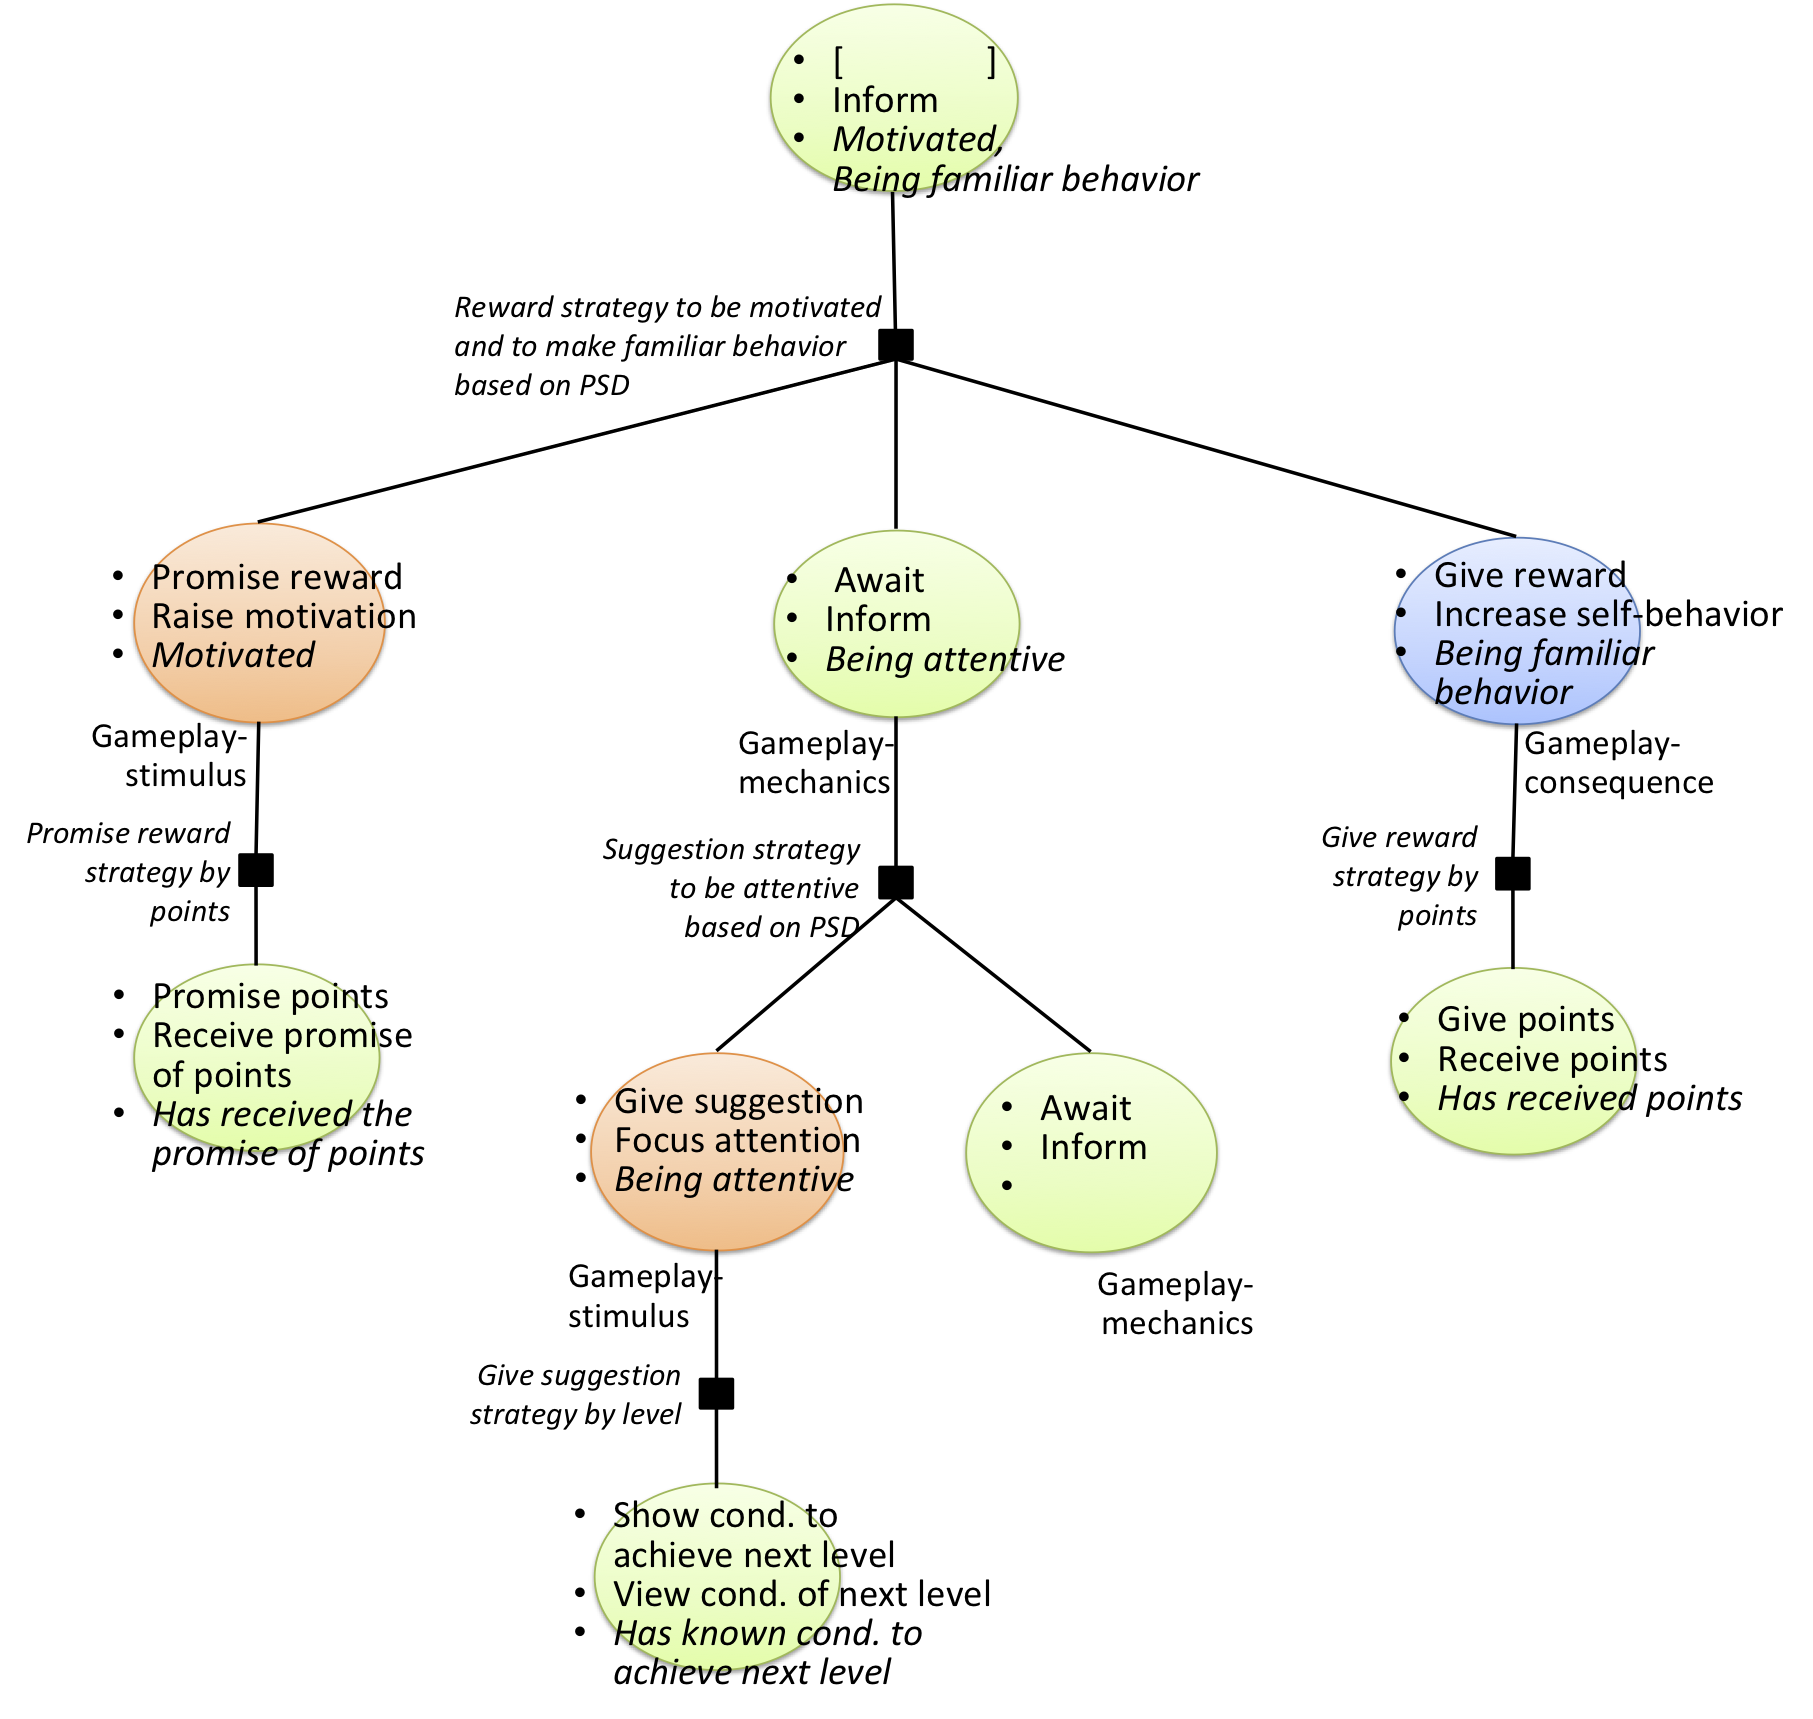
\includegraphics[width=0.85\textwidth]{images/chap-ontogacles2/decomposition-tree-gamified-giving-information-scenario-model.png}
 \fautor
\end{figure}

\autoref{fig:ontological-structure-gamified-giving-information-scenario-model} presents the ontological structure formalized to represent the persuasive gameplay scenario model shown in \autoref{fig:decomposition-tree-gamified-giving-information-scenario-model}. According to this structure, the PGDS \aspas{\emph{Reward strategy to be motivated and to make familiar behavior based on PDS}} is represented as a link for a \emph{Gameplay event} and three \emph{micro}-gameplay events defined as a \emph{Gameplay-stimulus event}, a \emph{Gameplay-mechanism event}, and a \emph{Gameplay-consequence event}. In the \emph{macro}-gameplay event, the goals to be achieved by this PGDS are \aspas{\emph{Motivated}} and \aspas{\emph{Being familiar behavior}} defined as \emph{Terminal state} in the \emph{Non-game event} played by the instructional event \aspas{\emph{Giving information}.}
The GDS \aspas{\emph{Promise reward strategy by points}} is represented as a link between the \emph{macro}- and \emph{micro}-gameplay events defined by the game actions \aspas{\emph{Promise reward}} and \aspas{\emph{Promise points},} respectively. The \emph{Psycological effect} as terminal state for the action \aspas{\emph{Raise motivation}} in the \emph{Gameplay-stimulus event} defined as \emph{macro}-gameplay event is \emph{Motivated}, and the \emph{Terminal state} for the action \aspas{\emph{Receive promise of points}} defined in the \emph{micro}-gameplay event is \emph{Has received the promise of points}. 
The GDS \aspas{\emph{Give reward strategy by points}} is represented as a link between the \emph{macro}- and \emph{micro}-gameplay events defined by the game actions \aspas{\emph{Give reward}} and \aspas{\emph{Give points},} respectively. The \emph{Psycological effect} as terminal state for the action \aspas{\emph{Increase self-behavior}} in the \emph{Gameplay-consequence event} defined as \emph{macro}-gameplay event is \emph{Being familiar behavior}, and the \emph{Terminal state} for the action \aspas{\emph{Receive points}} defined in the \emph{micro}-gameplay event is \emph{Has received points}. 
The \emph{Gameplay-mechanism event} defined by the non-game event \aspas{\emph{Giving information}} is decomposed by the PGDS \aspas{\emph{Suggestion strategy to be attentive based on PSD}} into a \emph{Gameplay-stimulus event} and a \emph{Gameplay-mechanism event} to achieve the \emph{Terminal state} of \emph{Being attentive}. 
The \emph{Gameplay-stimulus event} defined by the game action \aspas{\emph{Give suggestion}} causes the \emph{Psychological effect} of \emph{Being attentive} by the psychological process \aspas{\emph{Focus attention}.}
This goal is accomplished by the GDS \aspas{\emph{Give suggestion strategy by level}} in which the game action \aspas{\emph{Show cond. to achieve the next level}} cause the action \aspas{\emph{View cond. of next level}} to achieve the \emph{Terminal state} of \emph{Has known cond. to achieve next level}.

\begin{figure}[!htb]
 \caption{Example of ontological structure to represent the gamification of \emph{Giving information}}
 \label{fig:ontological-structure-gamified-giving-information-scenario-model}
 \centering
 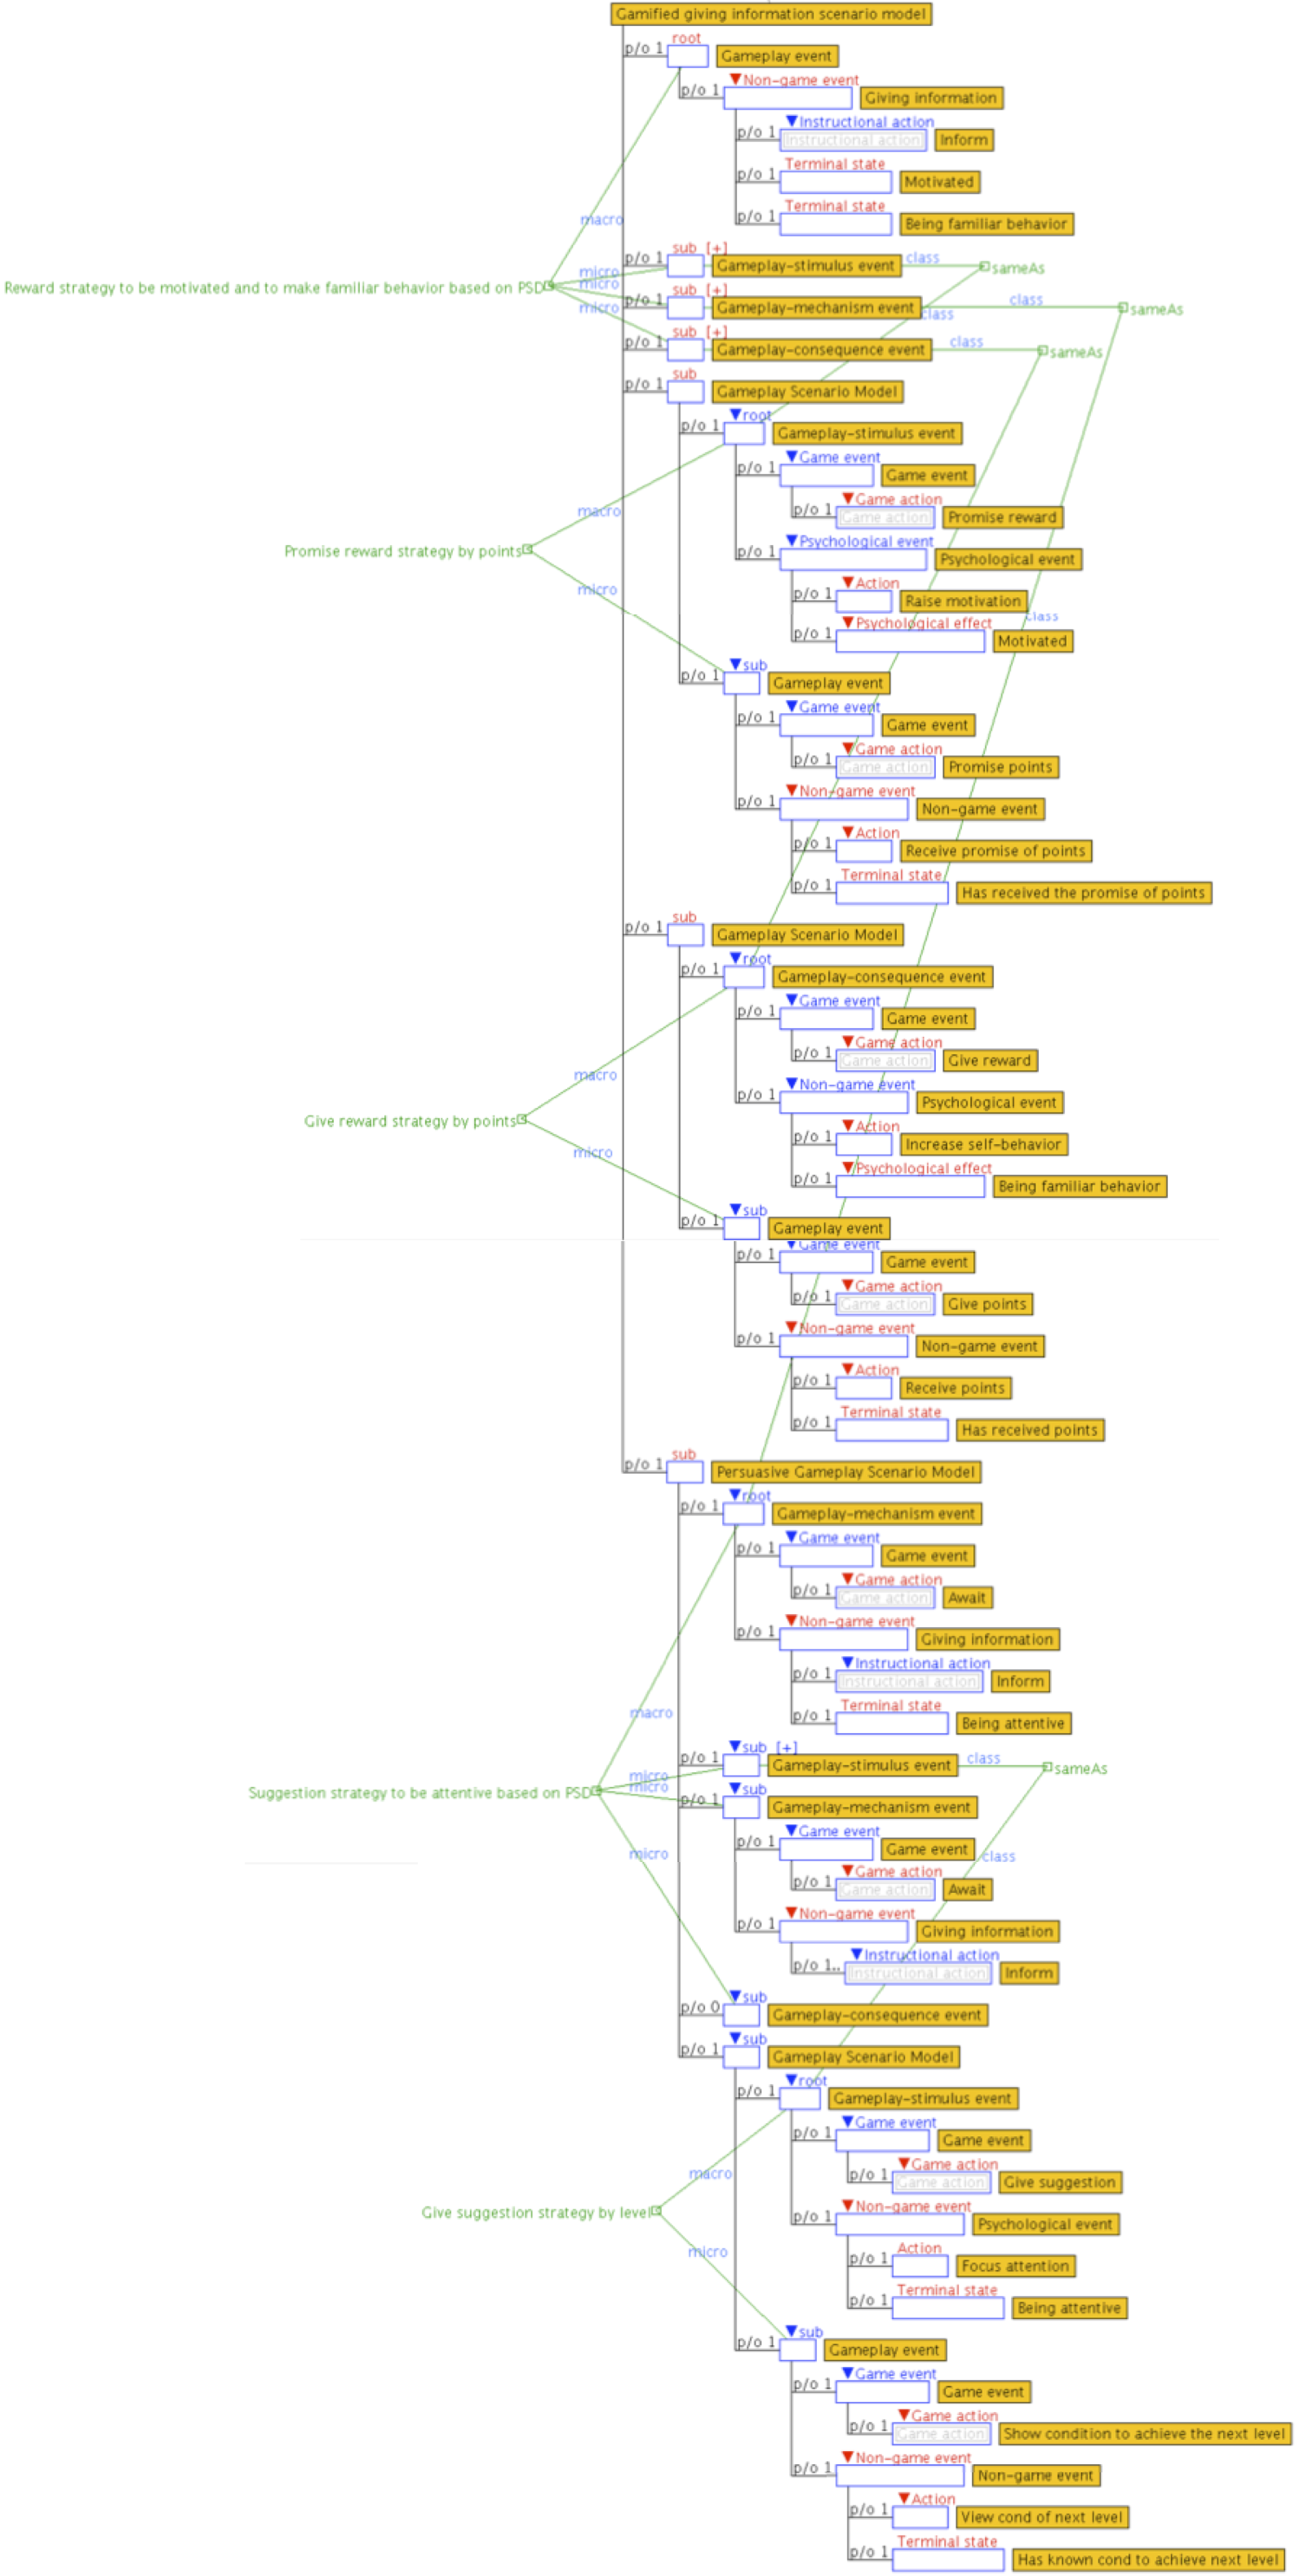
\includegraphics[width=0.7\textwidth]{images/chap-ontogacles2/ontological-structure-gamified-giving-information-scenario-model.png}
 \fautor
\end{figure}
\newpage

%%%%%%%%%%%%%%%%%%%%%%%%%%%%%%%%%%%%%%%%%%%%%%%%%%
\section[Modeling of CL Gameplay Based on Persuasive Game Design]{Modeling of Collaborative Learning Gameplay Based on Persuasive Game Design}
\label{sec:modeling-cl-gameplay-persuasive-game-design}

Having the ontological structures to represent Persuasive Game Design Strategies (PGDSs) and the rational design about how to successively apply them, we can procedure to link the design of CL process and the PGD for dealing with the motivation problem caused by the scripted collaboration. This link was established by the modeling of CL gameplay based on PGD. The concepts, terms and relations defined in this modeling are shown in \autoref{fig:concepts-terms-and-relation-in-cl-gameplay}, where:

\begin{description}
\item[Gamified I\_L event]
represents the influential I\_L event in which a set of PGDSs has been applied to persuade the participants who play the instructor and learner roles to interact between them performing the instructional and learning actions defined in an I\_L event.

\item[CL Game Dynamic]
describes the run-time behavior of game elements acting to persuade the participants to follow the interactions defined by the sequencing mechanism of a CSCL script. This behavior is defined by the PGDSs applied to interaction patterns.
 
\item[CL Gameplay]
is the set of CL Game dynamics defined in a gamified CL scenario to describe the whole CL process in a gamified CL scenario.
\end{description}


\begin{figure}[!htbp]
 \caption{Concepts, terms and relations in the modeling of CL gameplay based on PGD}
 \label{fig:concepts-terms-and-relation-in-cl-gameplay}
 \centering
 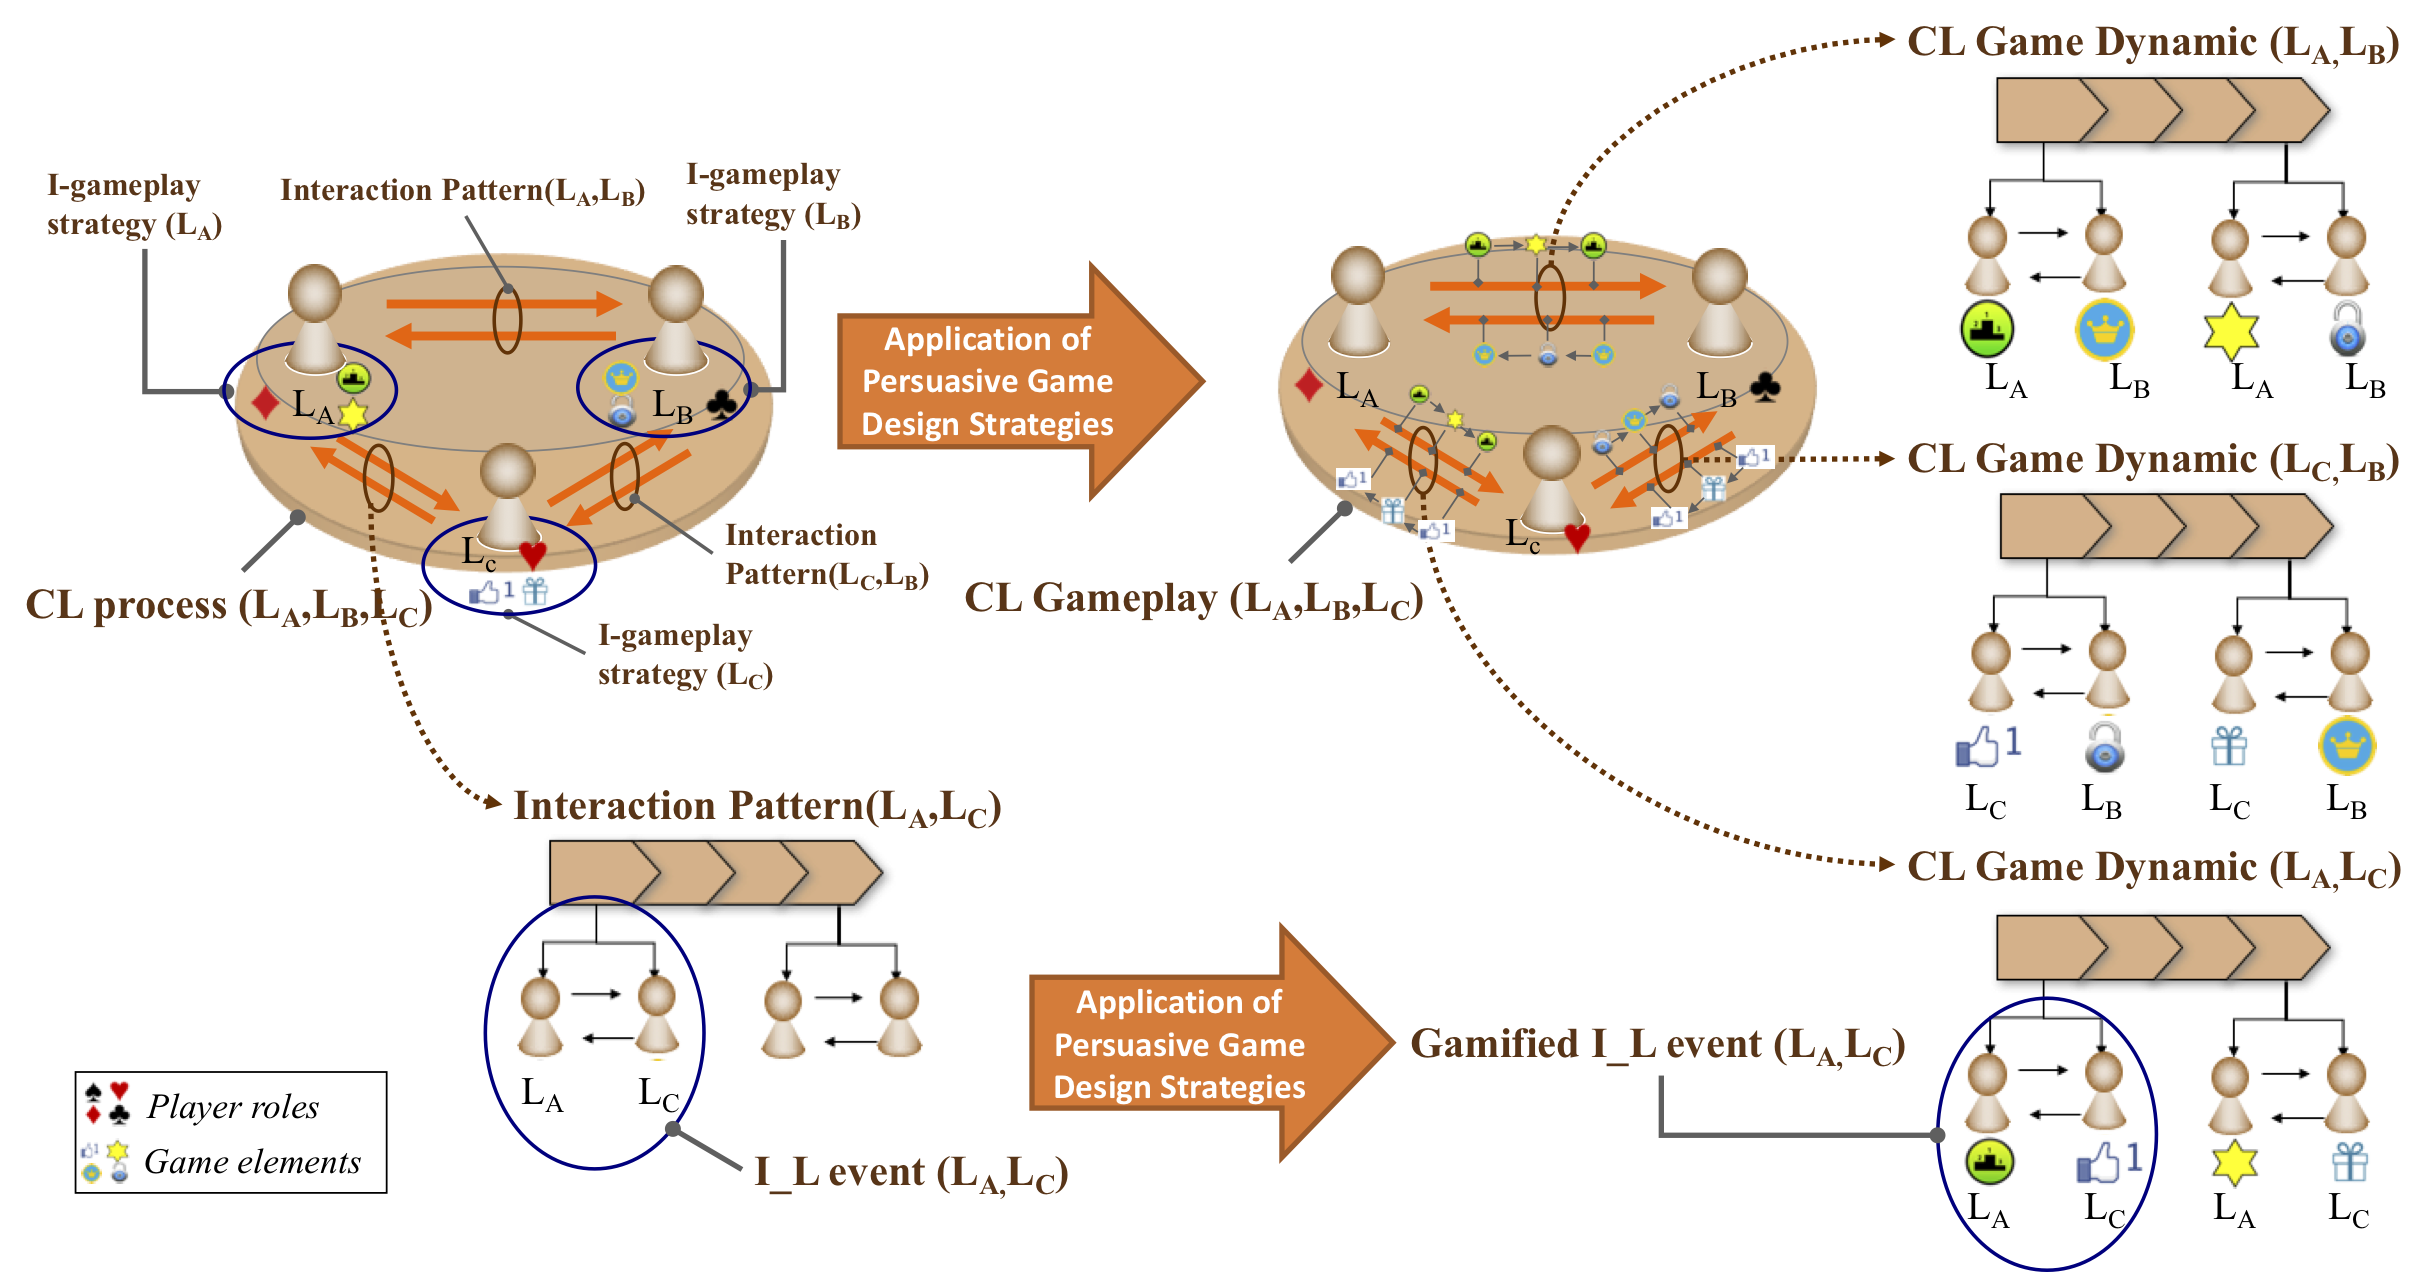
\includegraphics[width=1\textwidth]{images/chap-ontogacles2/concepts-terms-and-relation-in-cl-gameplay.png}
 \fautor
\end{figure}

In the following subsections, the formalization of concepts, terms and relations briefly introduced here are detailed.

\subsection{Gamified I\_L Event}
\label{subsec:gamified-il-event}

In the ontology OntoGaCLeS, the interaction defined by the sequencing mechanism of a CSCL script is represented by two parts: an \emph{Instructional event}, and a \emph{Learning event}. Thus, in a gamified CL scenario, as shown in \autoref{fig:gameplay-scenario-models-gamified-il-event}, the \emph{Gamified I\_L event} has been formalized an interaction composed by the pairs of events: \emph{Gamified instructional event}, and \emph{Gamified learning event}. These both events are result of applying PGDSs in the instructional and learning events as illustrated in the figure in which the \emph{Gameplay Scenario Model 1} corresponds to the instructional event, and the \emph{Gameplay Scenario Model 2} corresponds to the learning event.

\begin{figure}[!htbp]
 \caption{Elements in a gamified I\_L event}
 \label{fig:gameplay-scenario-models-gamified-il-event}
 \centering
 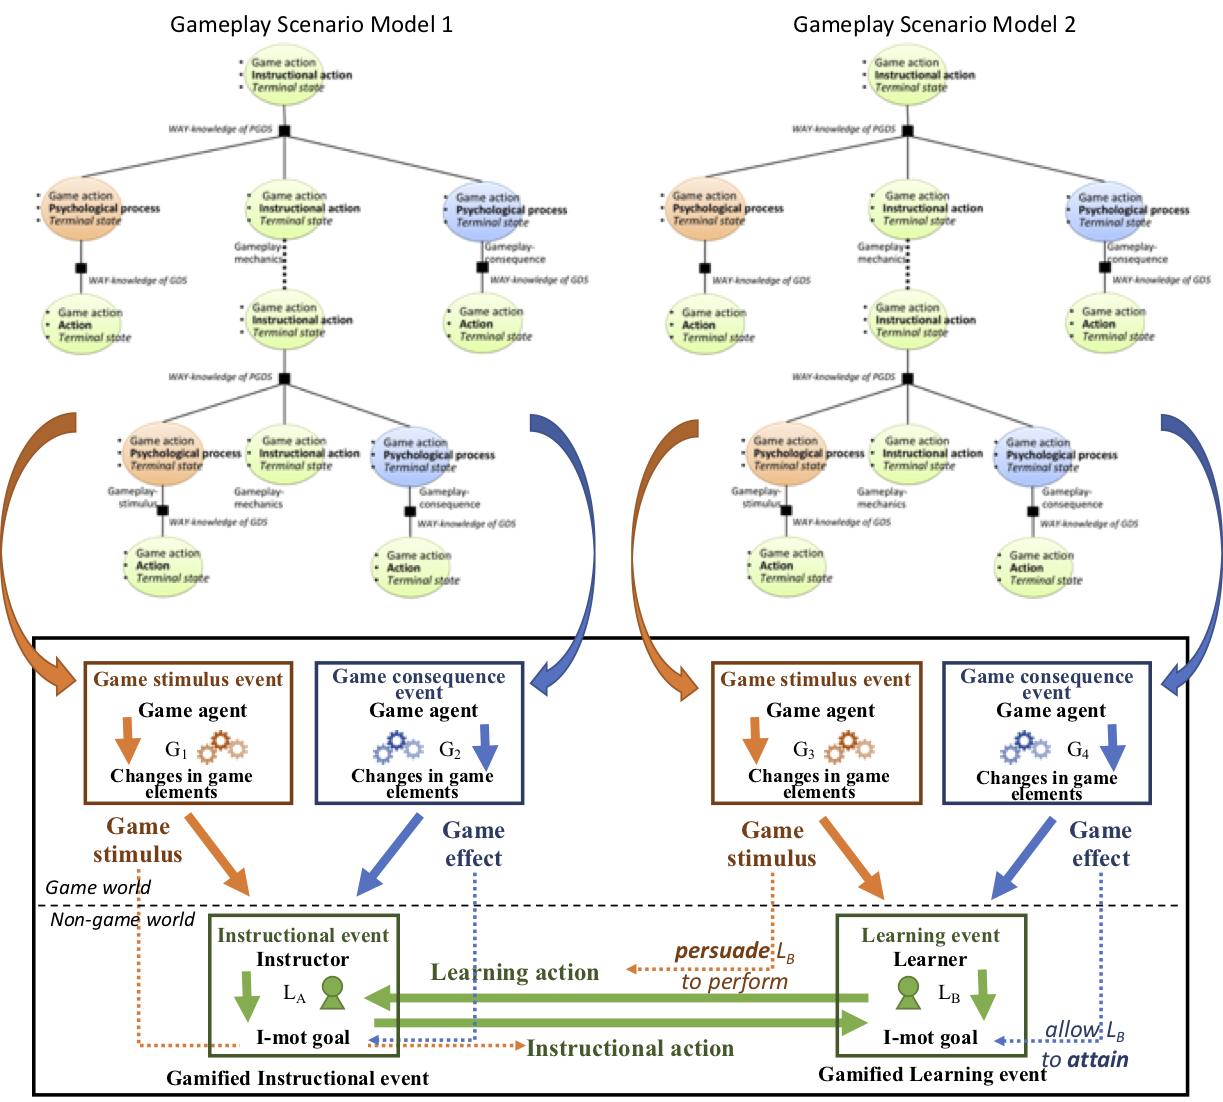
\includegraphics[width=1\textwidth]{images/chap-ontogacles2/gameplay-scenario-models-gamified-il-event.png}
 \fautor
\end{figure}

The gameplay scenarios in a gamified I\_L event describe the design rationales whereby the instructional and learning events are gamified to influence the instructor and learner role holders to perform the action indicated by the sequencing mechanism of CSCL script. Such influence is caused by game actions that occur before and after the instructional and learning actions defined in the instructional and learning events. As shown in \autoref{fig:gameplay-scenario-models-gamified-il-event}, when these game actions are derived from gameplay-stimulus events occurring before the instructional and learning actions, they become \emph{game stimulus}; and when these game actions are derived from gameplay-consequence events occurring after the instructional and learning actions, they become \emph{game effects}. The game stimulus, the game agents ($G_{1}$ and $G_{3}$) performing these stimulus, and the changes in game elements caused by the game stimulus are formalized as game stimulus events. The game effects, the game agents ($G_{2}$ and $G_{4}$) performing these effects, and the changes in game elements caused by the game effects are formalized as game consequence events. In these sense, the game actions as game stimulus carried out by the game agents ($G_{1}$ and $G_{3}$) \emph{persuade} the instructor ($L_{A}$) and learner ($L_{B}$) to perform the instructional and learning actions indicated in the instructional and learning events. The game actions carried out by the game agents ($G_{2}$ and $G_{4}$) are game effects that allow to the instructor ($L_{A}$) and ($L_{B}$) to \emph{attain} individual motivational goals (\emph{I-mot goal}). These individual motivational goals represent the expected changes in the motivational stage of participants ($L_{A}$ and $L_{B}$) to interact between them.

The ontological structure proposed in the ontology OntoGaCLeS to represent a \aspas{\emph{Gamified I\_L event}} is shown at the top of \autoref{fig:ontological-structure-gamified-il-event}. According to this structure, the role of \emph{Gamified I event} is played by a \emph{Gamified instructional event}, and the role of \emph{Gamified L event} is played by a \emph{Gamified learning event}. The \emph{Gamified instructional event} is composed by: a \emph{Game stimulus event} played by a \emph{Game event}, a \emph{Game consequence event} played by a \emph{Game event}, and a \emph{Game mechanism event} played by an \emph{Instructional event}. The \emph{Gamified learning event} is composed by: a \emph{Game stimulus event} played by a \emph{Game event}, a \emph{Game consequence event} played by a \emph{Game event}, and a \emph{Game mechanism event} played by a \emph{Learning event}. The instructional and learning events become game mechanism events because, when these events are gamified by the application of PGDSs, the instructional and learning actions are game mechanisms invoked by the instructor and learner to push forward through the game elements, and thus, to \emph{attain} individual motivational goals (\emph{I-mot goal}). These individual motivational goals are represented in the ontological structure as \emph{Benefits for the player} that can be achieved by the instructor and learner by performing the actions indicated in the instructional and learning events. The link \aspas{\emph{persuade}} in the \emph{Gamified I event} and \emph{Gamified L event} indicates the relation concept between game stimulus and instructional/learning actions. This link represents the instructional and learning actions influenced by persuasion and/or social influence. The link \aspas{\emph{attain}} in these both gamified events (\emph{Gamified I event} and \emph{Gamified L event}) indicates the relation concept between game effects and individual motivational goals (\emph{I-mot goal}) in which the game effects are actions that allow the learner and instructor to accomplish the individual motivation goals.

\begin{figure}[!htbp]
 \caption[Ontological structure to represent a \emph{Gamified I\_L event}]{Ontological structure to represent a \aspas{\emph{Gamified I\_L event}} (at the top). At the bottom, an example of Gamified I\_L event \aspas{\emph{Gamified Notify how the learner is}} as ontological structure.}
 \label{fig:ontological-structure-gamified-il-event}
 \centering
 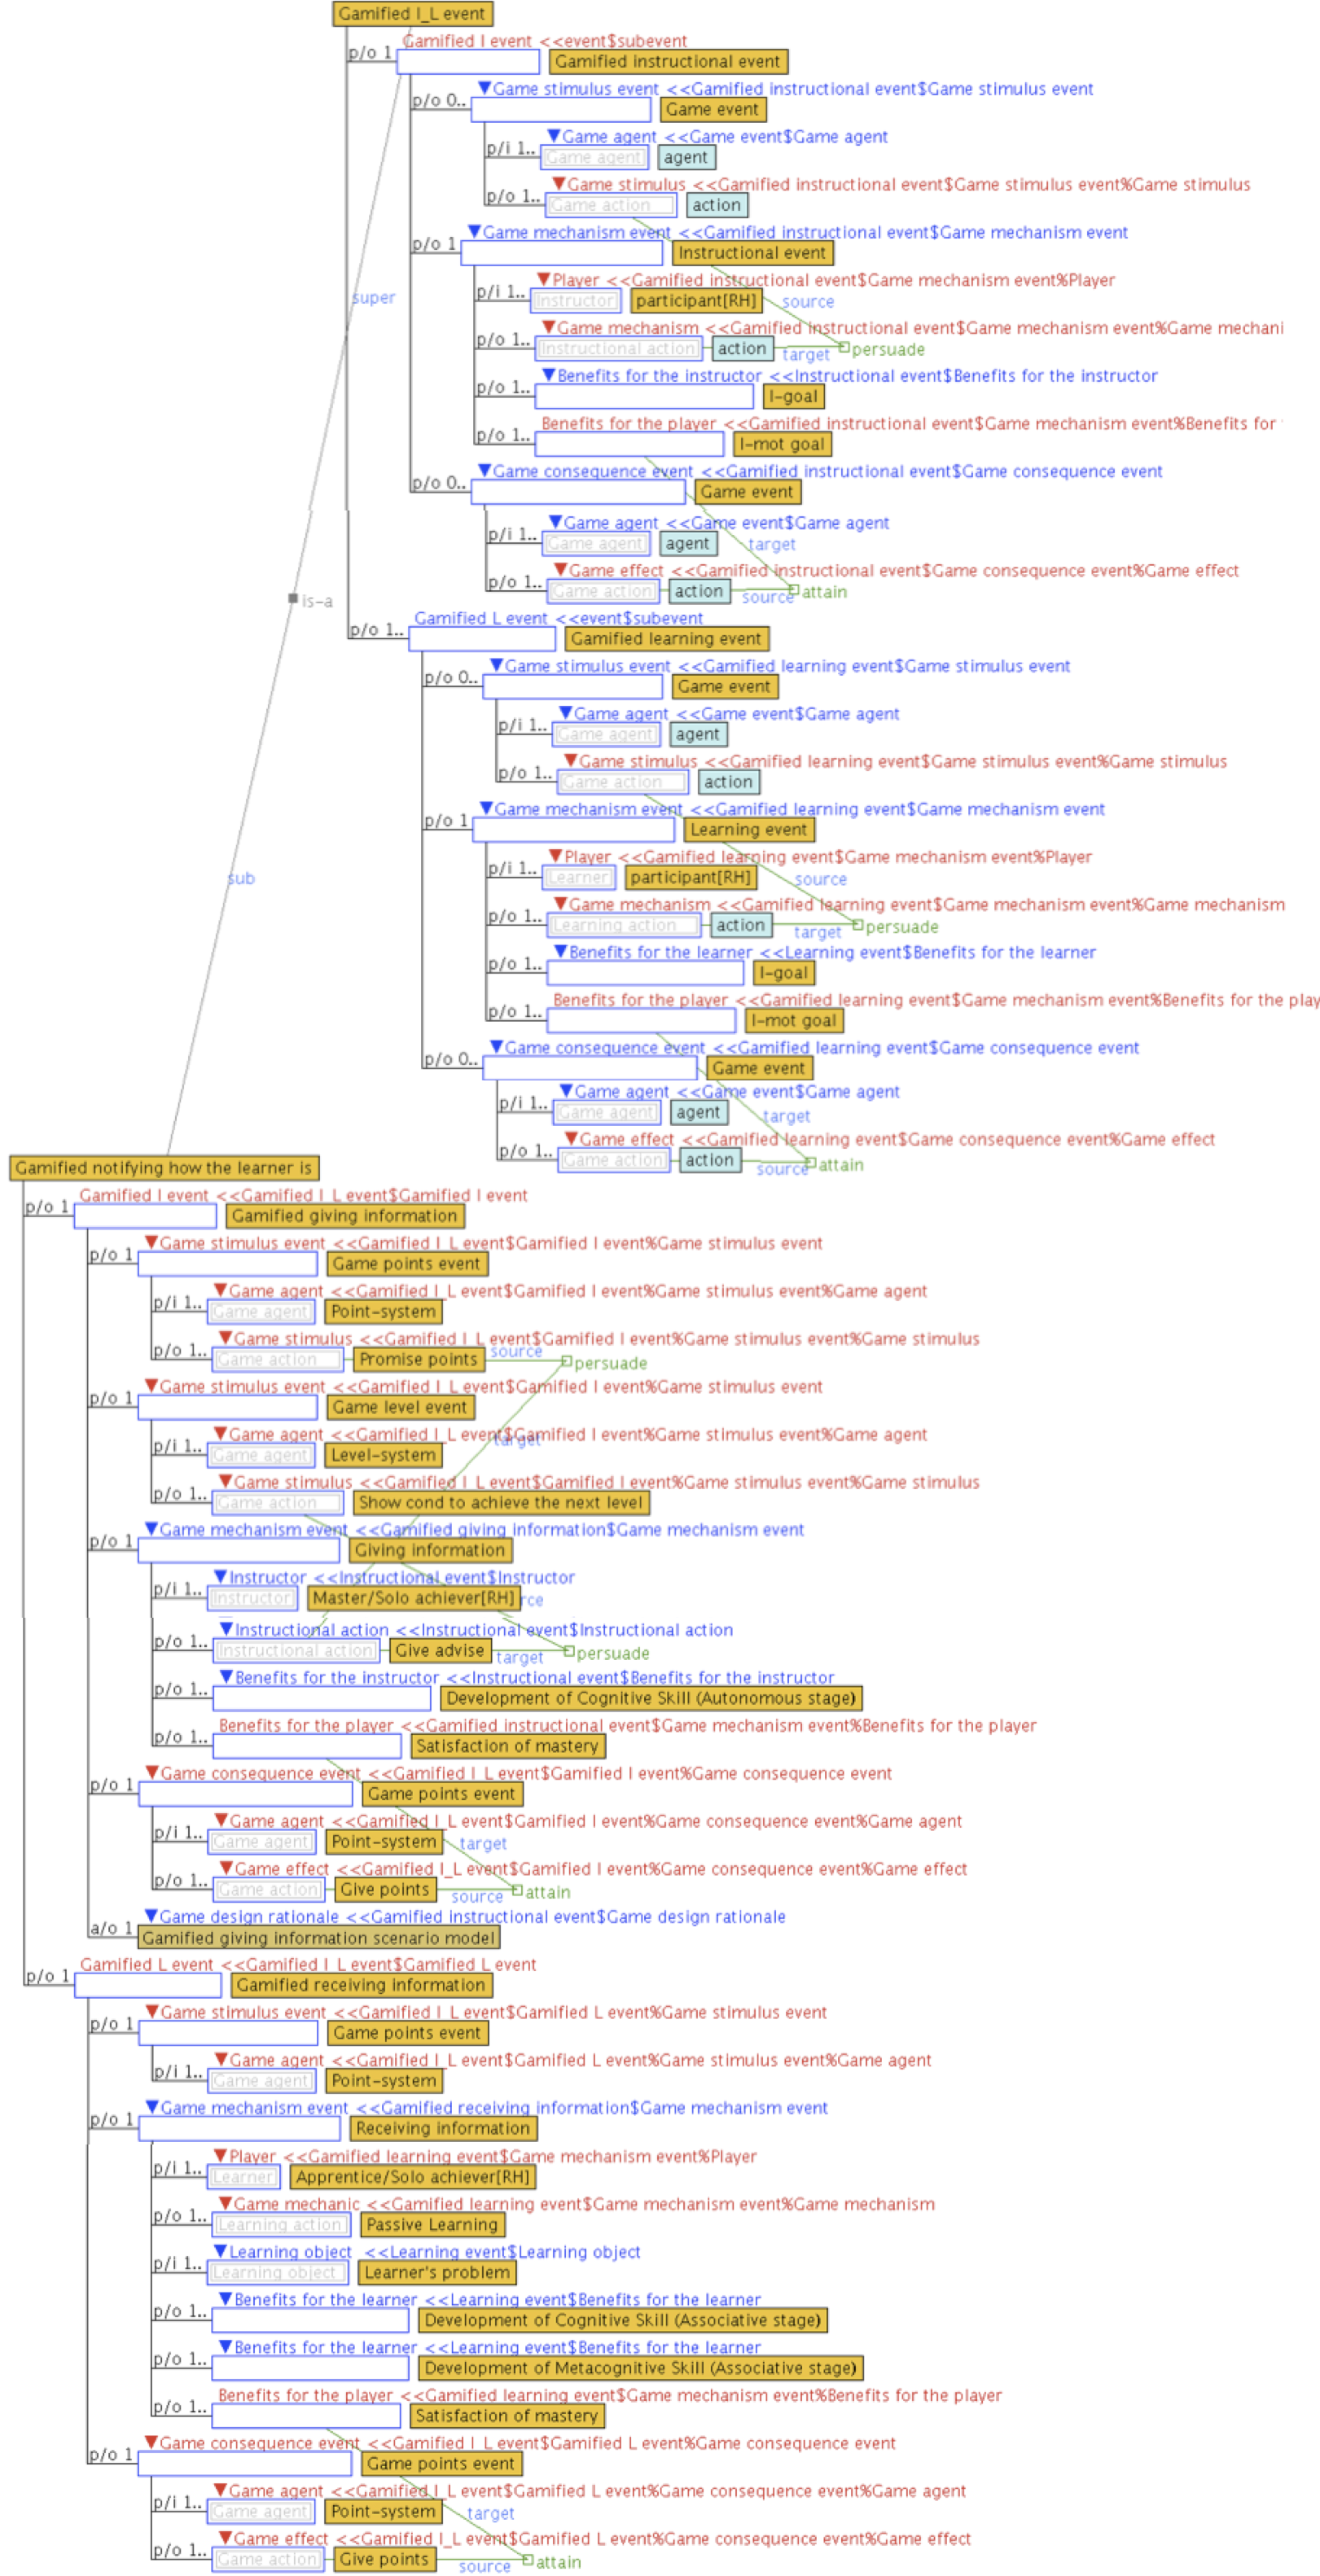
\includegraphics[width=0.74\textwidth]{images/chap-ontogacles2/ontological-structure-gamified-il-event.png}
 \fautor
\end{figure}
\newpage

At the bottom of \autoref{fig:ontological-structure-gamified-il-event}, there is shown the ontological structure to represent a Gamified I\_L event \aspas{\emph{Gamified Notify how the learner is}} illustrated in \autoref{fig:elements-gamified-notify-how-learner-is}. This ontological structure is result of applying the PGDSs and GDSs of \emph{Gameplay Scenario Model 1} and \emph{Gameplay Scenario Model 2} for the Instructional event \aspas{\emph{Giving information}} and the Learning event \aspas{\emph{Receiving information}.} The \emph{Gameplay Scenario Model 1} is indicated as the attribute \aspas{\emph{Game design rationale}} in the \emph{Gamified giving information}. According to this game design rationale, a game points event becomes game stimulus event when the game action \aspas{\emph{Promise points}} as game stimulus carried out by the \emph{Point-system} persuades the \emph{Master/Solo achiever role holder} as instructor to perform the instructional action \aspas{\emph{Give advise}} that becomes game mechanism. A game level event becomes game stimulus event when the game action \aspas{\emph{Show cond. to achieve the next level}} as game stimulus carried out by the \emph{Level-system} persuades the \emph{Master/Solo achiever role holder} as instructor to perform the instructional action \aspas{\emph{Give advise}} that becomes game mechanism. The game points event becomes game consequence event when the game action \aspas{\emph{Give points}} performed by the \emph{Point-system} allows the \emph{Master/Solo achiever role holder} as instructor to \emph{attain} the \emph{Satisfaction of mastery} defined as \emph{Benefits for the player}.

\begin{figure}[!htbp]
 \caption[Elements in the example of gamified I\_L event \aspas{\emph{Gamified Notify how the learner is}.}]{Elements in an example of gamified I\_L event \aspas{\emph{Gamified Notify how the learner is}.}}
 \label{fig:elements-gamified-notify-how-learner-is}
 \centering
 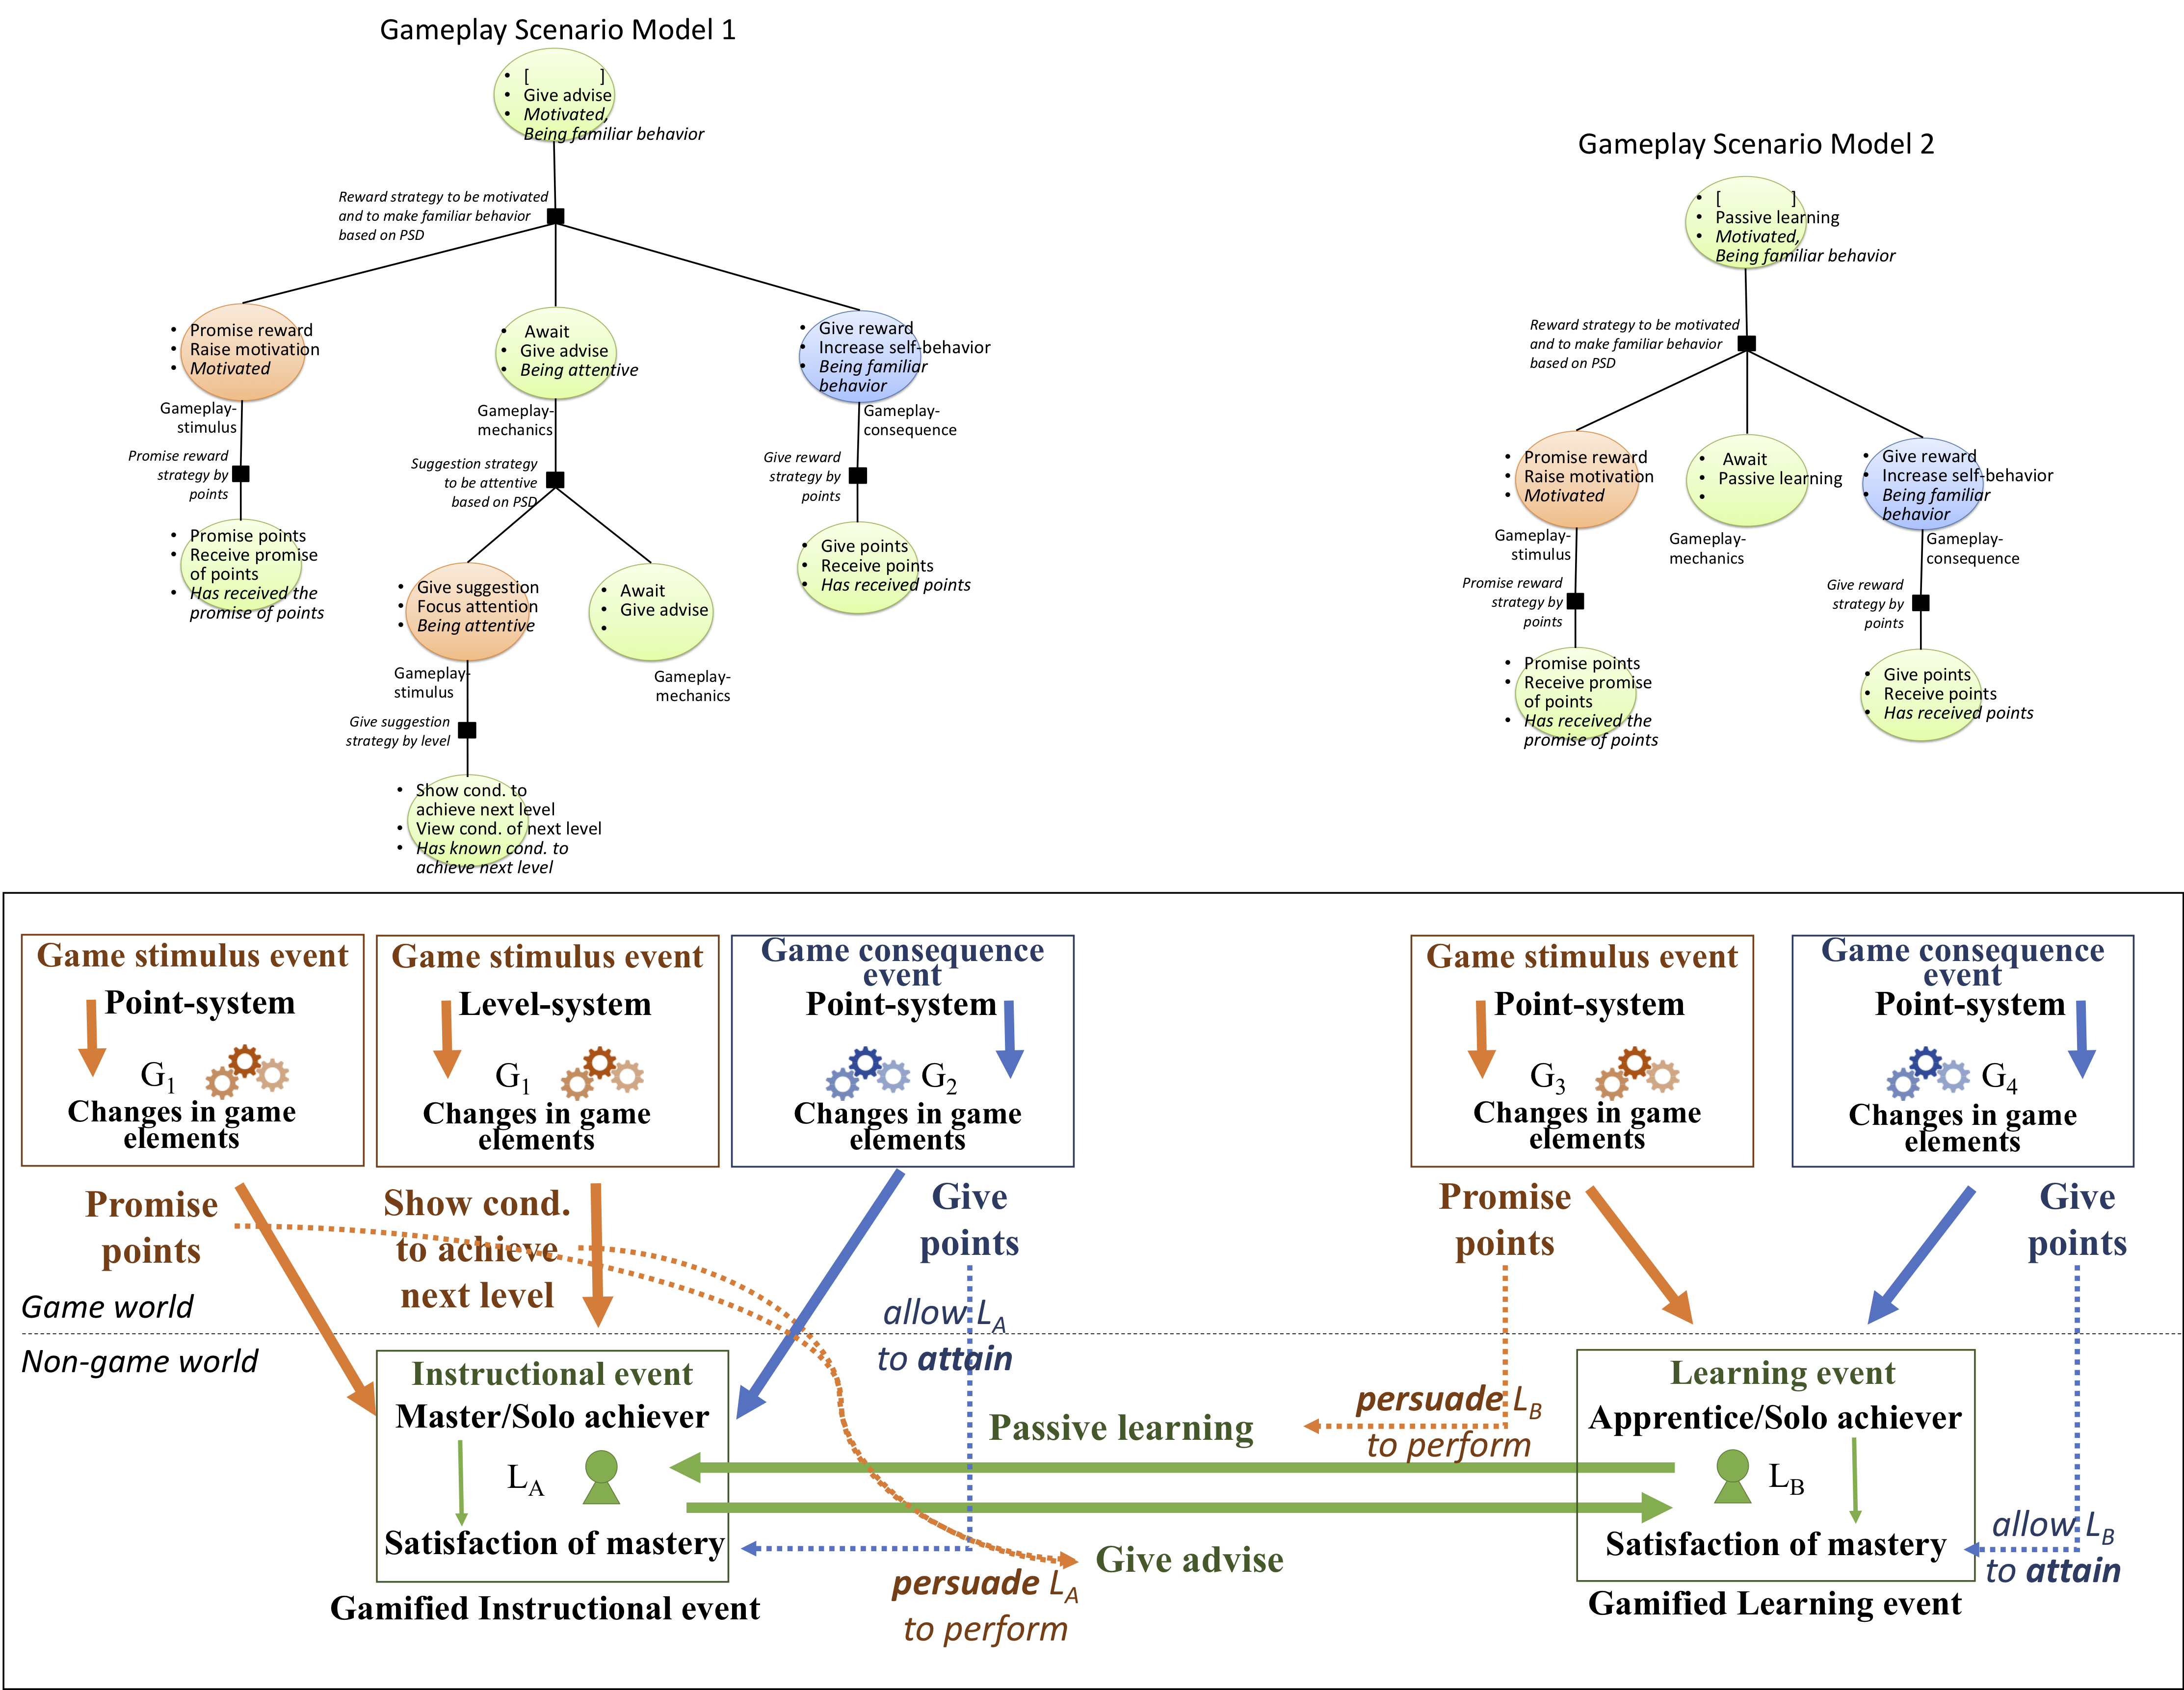
\includegraphics[width=1\textwidth]{images/chap-ontogacles2/elements-gamified-notify-how-learner-is.png}
 \fautor
\end{figure}

Having the representation of gamified I\_L events using ontological structures, there is the possibility to use the information contained in these structures to setting up the game elements introduced in the CL scenario being gamified. Because the information is explicitly and formally represented in the ontological structures, the designer can use this information to establish the interactions between the game elements and participants in a CL scenario. Thus, for the gamified I\_L event \aspas{\emph{Gamfied Notify how the learner is}} shown as an ontological structure at the bottom of \autoref{fig:ontological-structure-gamified-il-event} and with the elements illustrated in \autoref{fig:elements-gamified-notify-how-learner-is}, the interactions between participants and game elements can be established in the CL scenario according to the storyboard shown in \autoref{fig:storyboard-gamified-notify-how-learner-is}. In this sense, the game actions \aspas{\emph{Promise points}} and \aspas{\emph{Show cond. to achieve next level}} indicated in the ontological structure as game stimulus are defined as the messages \aspas{\emph{Give advice, and gain +200 points}} and \aspas{\emph{400 points to achieve 2nd level}} to be given by a point-system and a level-system as shown in the screens (1A) and (1B). These both message must be displayed in the system before the instructional action \aspas{\emph{Give advice}} defined in the ontological structure as a game mechanism. Such instructional action is defined in the system as a message \aspas{\emph{Give advice indicating the learner's problem}} and an interactive form to be filled by the \emph{Master/Solo achiever role holders}. The game action \aspas{\emph{Give points}} formalized as a game consequence in the ontological structure is setting up as the assignment of points and the message to be given to the \emph{Master/Solo achiever role holders} by the point-system as shown in the screen (3).

\begin{figure}[!htbp]
 \caption{Storyboard for the interactions between game elements and participants defined according to the example of gamified I\_L event \aspas{\emph{Gamified Notify how the learner is}.}}
 \label{fig:storyboard-gamified-notify-how-learner-is}
 \centering
 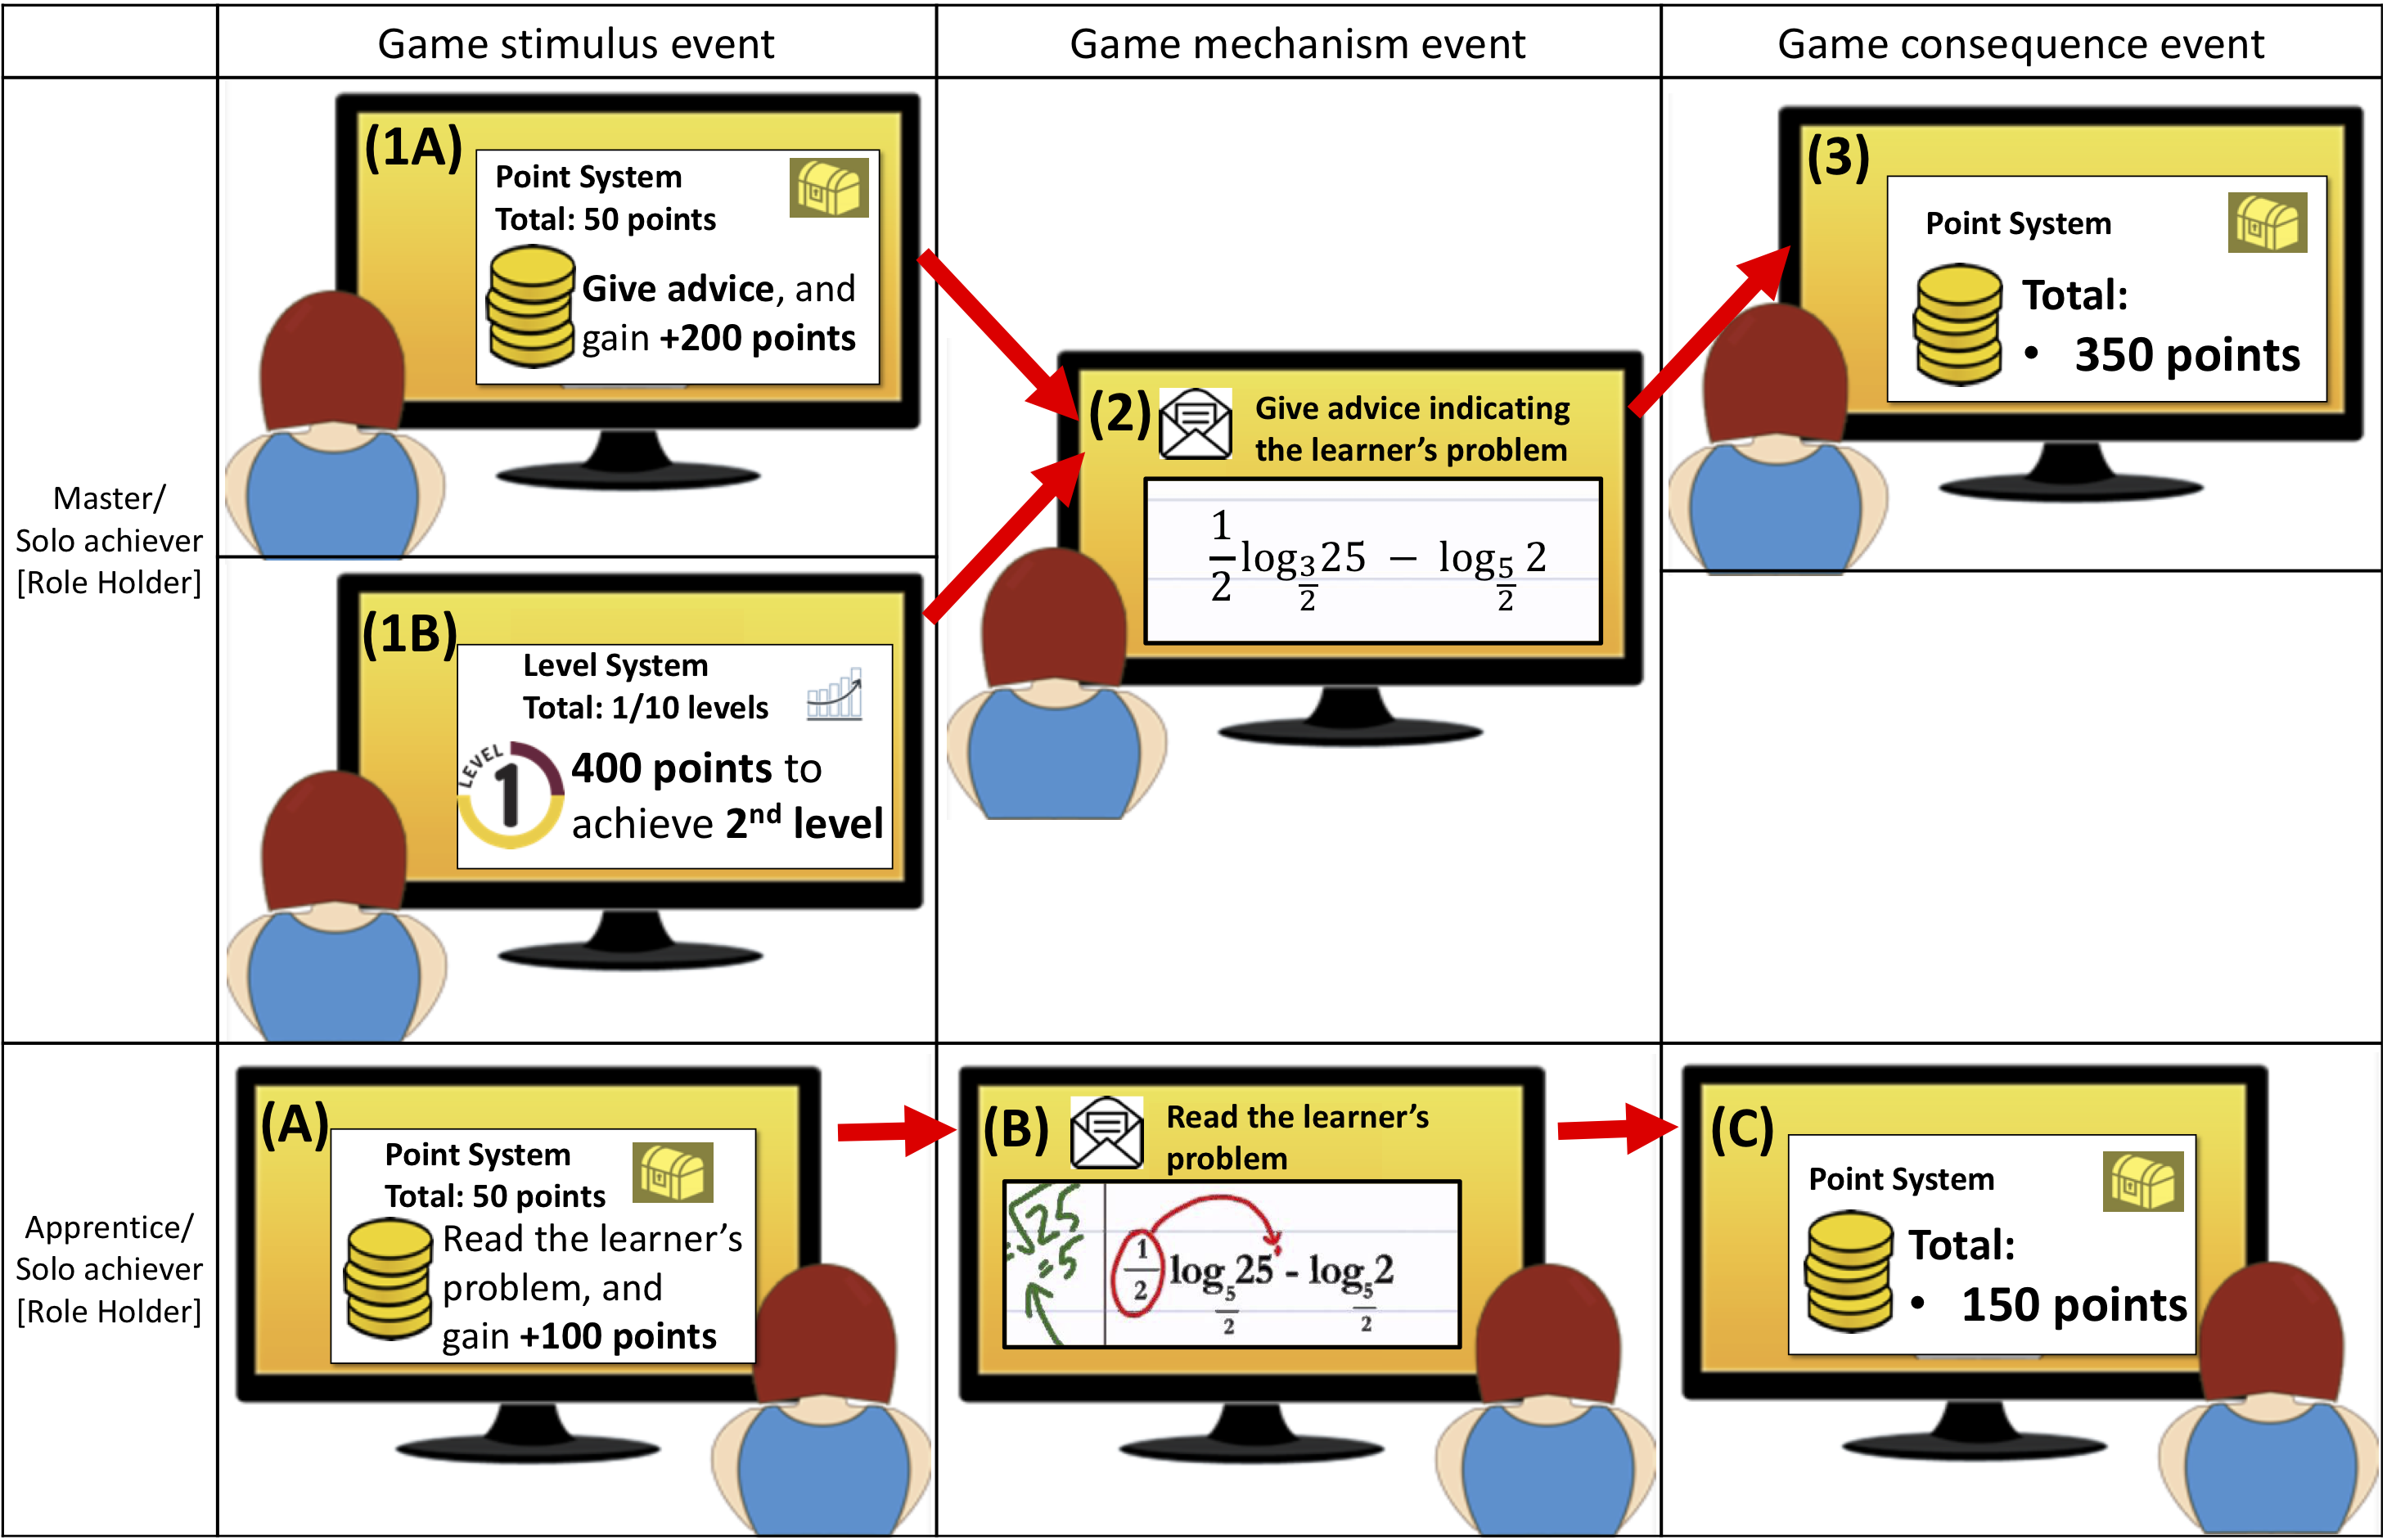
\includegraphics[width=0.85\textwidth]{images/chap-ontogacles2/storyboard-gamified-notify-how-learner-is.png}
 \fautor
\end{figure}

The configuration of game elements in the system for the \emph{Apprentice/Solo achiever role holders} is established as shown in the screens (A), (B) and (C) of \autoref{fig:storyboard-gamified-notify-how-learner-is}. This configuration is established according to the information provided by the ontological structure shown at the bottom of \autoref{fig:ontological-structure-gamified-il-event}. In this sense, the game action \aspas{\emph{Promise points}} as game stimulus is setting up as the message \aspas{\emph{Read the learner's problem and gain +100 points}} to be given by the point-system (Screen (A)), and the game action \aspas{\emph{Give points}} as game consequence is defined as the assignment of points and the message to be given by the point-system (Screen (C)).

The task of setting up the game actions to be performed by the game agents can be supported by an intelligent system that is able to reason on ontologies. Thus, the designer just needs to have a clear idea of individual motivational goals (\emph{I-mot goal}) to be achieved by the instructor and learner in the gamified I\_L event. These individual motivational goals represented as the expected \emph{Benefits for the players} in the ontological structures provide information to the intelligent system to find the game action that support the achievement of these benefits. These game actions are actions indicated as game stimulus and game consequences in the gamified I\_L event, and they can be found by the intelligent system when it has the information of player roles and individual motivational goals assigned for the instructor and learner in a gamified CL scenario. This process of extracting this information and how this information is used to setting up the game elements will be detailed in the \autoref{chapter:computer-based-mechanisms-procedures}.

\subsection{CL Game Dynamic}
\label{subsec:cl-game-dynamic}

According to the MDA framework proposed by \citeonline{HunickeLeBlancZubek2004}, the \aspas{\emph{Game dynamic describes the run-time behavior of the mechanics acting on player inputs and each others' outputs over time}} in which the mechanics describes the particular components of the game, at the level of data representation and algorithms. These mechanics have been represented as game agents in the ontological structures to represent game events as game stimulus and game consequence events in the gamified I\_L event. Thus, to describe the run-time behavior of these agents in a chunk of the CL process, in the ontological structure to represent a \emph{Gamified I\_L event}, the game events as \emph{game stimulus event} and \emph{game consequence event} include the description of these changes as object produced by the game actions and as states to be achieved by the game actions. The green frame of \autoref{fig:ontological-structure-cl-game-dynamic} shows part of the formalization of the run-time behavior of the game agents in the game consequence events of a gamified instructional event. As can be appreciated in the ontological structure to represent the CL Game dynamic, in the game stimulus event, the \emph{object} produced by the game action becomes \emph{Game component}, and the \emph{state} achieved by the game action becomes \emph{Game state}.

The piece of the whole CL process delimited by a gamified I\_L event is an interaction defined by the sequencing mechanism of a CSCL script. Thus, to represent the game dynamic in the whole CL process, the concept of \aspas{\emph{CL Game dynamic}} has been formalized in the ontology OntoGaCLeS as \aspas{\emph{the run-time behavior of the game agents acting to persuade the participants to follow the interactions defined by the sequencing mechanism of a CSCL script}.} At the top of \autoref{fig:ontological-structure-cl-game-dynamic} is shown the ontological structure to represent the CL Game dynamic in which the necessary and desired interactions are defined as roles that can be played by \emph{Gamified I\_L event}. These interactions are defined from interaction patterns formalized in the CL ontology in which the interaction patterns are specialization of CSCL scripts inspired by instructional/learning theories. An example of CL Game dynamic defined for the interaction pattern based on Cognitive Apprenticeship theory is shown at the bottom of \autoref{fig:ontological-structure-cl-game-dynamic}. In this ontological structure named as \aspas{\emph{Gamified Cognitive Apprenticeship type IP},} the necessary interactions are: \emph{Gamified setting up learning context type CA}, \emph{Gamified demonstrating how to solve a problem}, \emph{Gamified monitoring}, and \emph{Gamified affirmative reaction}. The desired interactions are: \emph{Gamified clarifying the problem}, \emph{Gamified notifying how the learner is}, \emph{Gamified instigating thinking}, \emph{Gamified requesting problem's details}, and \emph{Gamified showing a solution type CA}.

\begin{figure}[!htbp]
 \caption[Ontological structure to represent a \emph{CL Game dynamic}]{Ontological structure to represent the \aspas{\emph{CL Game dynamic}} (at the top). At the bottom, the ontological structure to represent a CL Game dynamic defined for the gamification of Cognitive Apprenticeship interaction pattern.}
 \label{fig:ontological-structure-cl-game-dynamic}
 \centering
 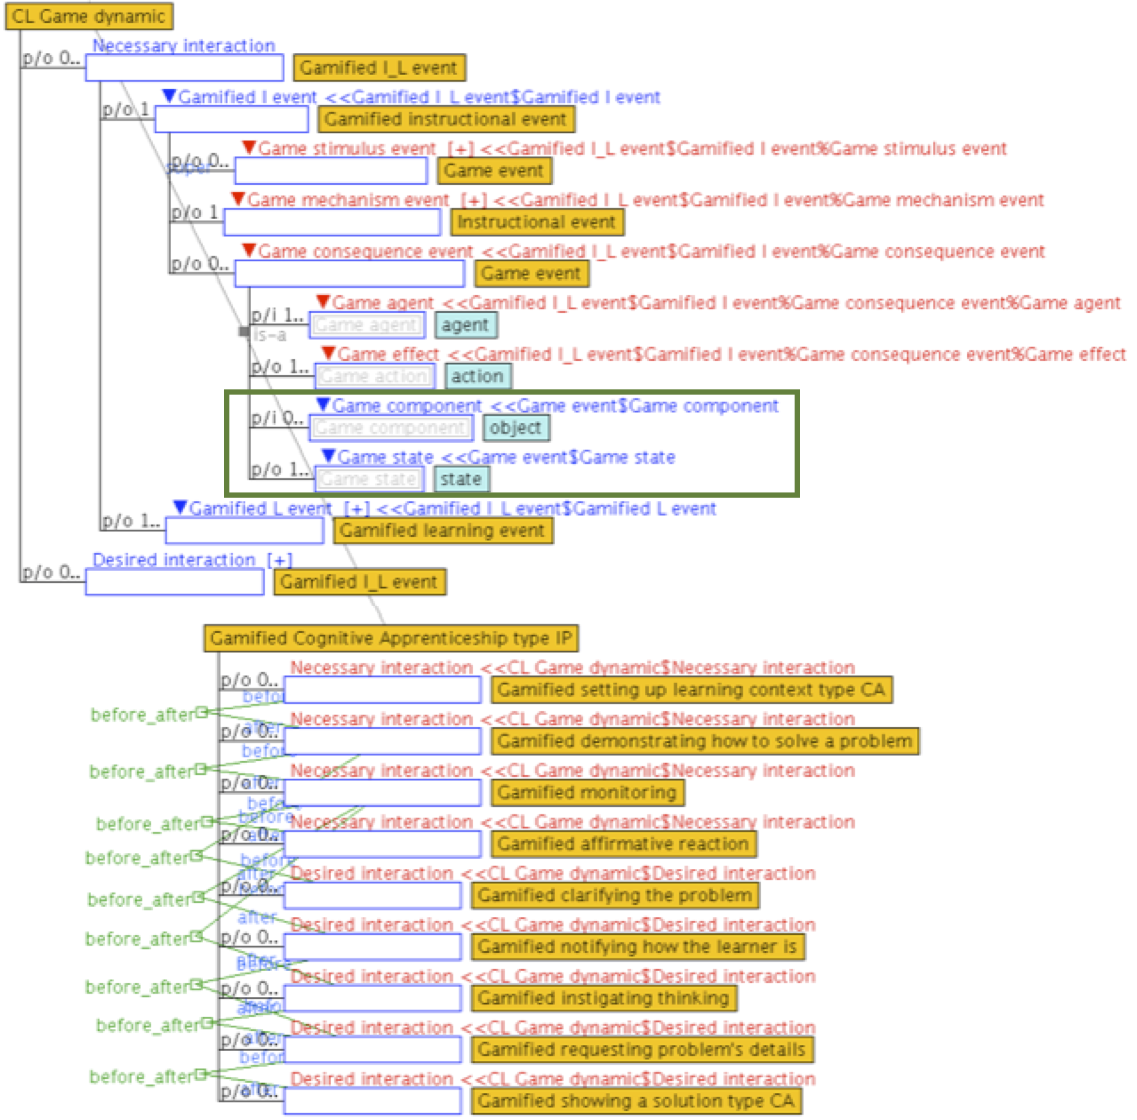
\includegraphics[width=1\textwidth]{images/chap-ontogacles2/ontological-structure-cl-game-dynamic.png}
 \fautor
\end{figure}

\subsection{CL Gameplay}
\label{subsec:cl-gameplay}

Beside the concept of gameplay is extensively talked in the literature related to game design and gamification, there is no one universally accepted definition of gameplay. According to \citeonline{FabricatoreNussbaumRosas2002}, gamers talk about gameplay when they refer to their experiences in the game focusing on what the player can do, what the game elements can do in response to the player's actions. Gameplay is the result of a large number of contributing elements \cite{RollingsAdams2003}, thereby \citeonline{DjaoutiAlvarezJesselMethelMolinier2008} defines gameplay as the way in which the players interact with a game elements by means of rules listening input and acting on game elements. These rules through the output system return to the player an evaluation of his performance observing the states of game elements. 

As the \emph{CL Game dynamic} describes the run-time behavior of game elements to persuade the participants to follow the sequencing mechanism of a CSCL script, the gameplay of a gamified CL scenario, defined as the concept of \aspas{\emph{CL Gameplay},} consists in the set of CL game dynamics defined in this scenario to cause changes in the participants' attitudes, intentions, motivation and/or behaviors. These changes are caused by the gameplay experience of participants interacting with the game elements through the CL Game dynamics. Thus, in the ontological structure to represent a \emph{Gamified CL Scenarios} as shown in \autoref{fig:ontological-structure-cl-gameplay}, the \emph{CL process} is replaced by the \emph{CL Gameplay}, where the information about \aspas{\emph{How to interact}} in the CL process described by an \emph{Interaction pattern} is replaced by the \emph{CL Game dynamic} playing the role \aspas{\emph{How to play}.} 

\begin{figure}[!htbp]
 \caption[Ontological structure to represent a \emph{Gamified CL Scenario}]{Ontological structure to represent a \aspas{\emph{Gamified CL Scenario}.}}
 \label{fig:ontological-structure-cl-gameplay}
 \centering
 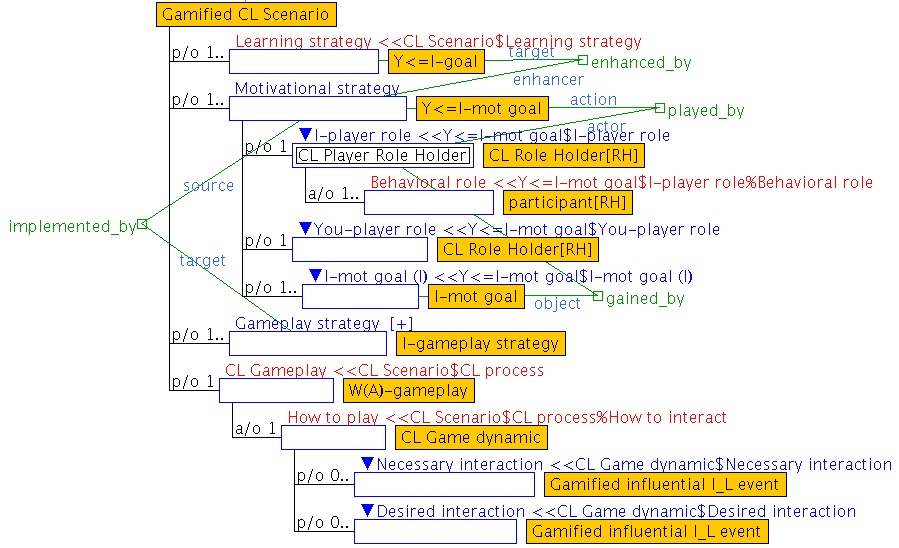
\includegraphics[width=0.95\textwidth]{images/chap-ontogacles2/ontological-structure-gamified-cl-scenario.png}
 \fautor
\end{figure}

%%%%%%%%%%%%%%%%%%%%%%%%%%%%%%%%%%%%%%%%%%%%%%%%%%
\section[Formalizing an Ontological Model to Apply Gamification as Persuasive Technology]{Formalizing an Ontological Model to Apply Gamification as Persuasive Technology in CL Scenarios}
\label{sec:formalizing-ontological-model-apply-gamification-persuasive-technology}

To demonstrate the applicability of the ontological structures presented in the previous sections, the building of an ontological model to apply gamification as persuasive technology in CL scenarios is detailed in this section. By gamification as persuasive technology, the author of this thesis refers to the use of game design elements to persuade and social influence the participants to change their attitudes, intentions, motivation and/or behaviors. Thus, an ontological model to apply gamification as persuasive technology in CL scenarios has the purpose to provide enough information for setting up the game elements to persuade the participants to follow the interactions defined by a CSCL script. The ontological model detailed here has been proposed to apply gamification as persuasive technology in CL scenarios based on the Cognitive Apprenticeship theory, and the information used to built this model comes from the Yee's model \cite{Yee2006} and Model-driven persuasive game proposed by \citeonline{Orji2014}.

The steps for building an ontological model to apply gamification as persuasive in CL scenarios are: (1) to identify the Persuasive Game Design Strategies (PGDSs) for player role holders who are in the \emph{primary focus} (P) and \emph{secondary focus} (S) of individual gameplay strategies (\emph{I-gameplay strategy}); (2) to apply the identified PGDSs in the interaction pattern; and (3) to define the game states and game components in the CL Game Dynamics to provide a gameplay experience according to the individual gameplay strategies.

\subsubsection*{Step (1): Identifying persuasive game design strategies for player role holders who are in the primary focus and secondary focus of individual gameplay strategies}

Several researchers have pointed the necessity to personalize the application of persuasive strategies due to the adverse reactions that can be caused in a person when inappropriate strategies are applied. For instance, a study of \citeonline{KapteinLacroixSaini2010} demonstrates that the use of non-tailored persuasive strategies produces negative reactions increasing the adoption of unhealthy behavior. Another example is the study carried out by \citeonline{OrjiVassilevaMandryk2014} in which the effectiveness of PGDSs for player types of BrainHex model was evaluated to identify the best and worst strategies to motivate health behavior change. Thus, to identifying the PGDSs for player role holders who are in the primary focus and secondary focus of individual gameplay strategies, it is necessary to have the list of PGDSs that cause positive and negative impacts in the player roles of ontological model being built.

\autoref{tab:persuasive-strategies-model-driven-persuasive-game} shows the (P)ositive and (N)egative  (counterproductive) impacts for the player types of BrainHex model identified in the Model-driven persuasive game proposed by \citeonline{Orji2014}. The PGDSs that cause the most (P)ositive and (N)egative impacts for  are indicated with bold texts. The relation of BrainHex player types with the component motivations identified in the Yee's model is indicated in the column \aspas{\emph{Yee's Model},} and it has been extracted from the study of \citeonline{NackeBatemanMandryk2014} in which, for instance, the BrainHex's Mastermind player type is related to the Yee's \emph{Mechanics} component motivation because people who are classified in these both player types enjoys to devise strategies for solving puzzles and problem, because they obtain pleasure when they make good decisions. The column \aspas{\emph{Player role}} indicates the relation between the PGDSs and the player roles based on the Yee's model.


\begin{quadro}[htb]
\caption{Persuasive game design strategies for player types of BrainHex and Yee's model}
\label{tab:persuasive-strategies-model-driven-persuasive-game}
\centering
\tiny
\begin{tabular}{|l|cccccccc|c|c|}
\hline

\multirow{2}{*}{\textbf{BrainHex}}&
\multirow{1}{*}{\textbf{CMPT/}}&
\multirow{2}{*}{\textbf{COOP}}&
\multirow{2}{*}{\textbf{CUST}}&
\multirow{2}{*}{\textbf{PERS}}&
\multirow{2}{*}{\textbf{PRAS}}&
\multirow{1}{*}{\textbf{SEMT/}}&
\multirow{2}{*}{\textbf{SIML}}&
\multirow{2}{*}{\textbf{REWD}}&
\multirow{2}{*}{\textbf{Yee's Model}}&
\multirow{2}{*}{\textbf{Player Role}}\tabularnewline
&
\multirow{1}{*}{\textbf{CMPR}}&
&
&
&
&
\multirow{1}{*}{\textbf{SUGG}}&
&
&
&
\tabularnewline
\hline

Achiever& &\textbf{(P)}& & & &(P)& &(P)&\emph{Advancement}&\multirow{3}{*}{Yee Achiever}\tabularnewline
Mastermind&(P)& &(P)&(P)& &\textbf{(P)}&(P)& &\emph{Mechanics}& \tabularnewline
Conqueror&\textbf{(P)}& & &(P)& &(P)&(P)& &\emph{Competition}& \tabularnewline
\hline

Socializer&(P)&\textbf{(P)}&(N)& &(N)&\textbf{(N)}& & &\emph{Social}&Yee Socializer\tabularnewline
\hline

Seeker&(P)& &\textbf{(P)}&(P)&(P)& & & &\emph{Immersion}&\multirow{3}{*}{Dreamer}\tabularnewline
Survivor&(P)&\textbf{(N)}&(N)& & &\textbf{(P)}& &(N)&\emph{Escapism}& \tabularnewline
Daredevil&(N)& & & & &\textbf{(N)}&\textbf{(P)}& &\emph{Escapism}& \tabularnewline
\hline

Achiever& &\textbf{(P)}& & & &(P)& &(P)&\emph{Advancement}&\multirow{4}{*}{Social Achiever}\tabularnewline
Mastermind&(P)& &(P)&(P)& &\textbf{(P)}&(P)& &\emph{Mechanics}& \tabularnewline
Conqueror&\textbf{(P)}& & &(P)& &(P)&(P)& &\emph{Competition}& \tabularnewline
Socializer&(P)&\textbf{(P)}&(N)& &(N)&\textbf{(N)}& & &\emph{Social}&\tabularnewline
\hline

Achiever& &\textbf{(P)}& & & &(P)& &(P)&\emph{Advancement}&\multirow{6}{*}{Achiever Dreamer}\tabularnewline
Mastermind&(P)& &(P)&(P)& &\textbf{(P)}&(P)& &\emph{Mechanics}& \tabularnewline
Conqueror&\textbf{(P)}& & &(P)& &(P)&(P)& &\emph{Competition}& \tabularnewline
Seeker&(P)& &\textbf{(P)}&(P)&(P)& & & &\emph{Immersion}&\tabularnewline
Survivor&(P)&\textbf{(N)}&(N)& & &\textbf{(P)}& &(N)&\emph{Escapism}& \tabularnewline
Daredevil&(N)& & & & &\textbf{(N)}&\textbf{(P)}& &\emph{Escapism}& \tabularnewline
\hline

Socializer&(P)&\textbf{(P)}&(N)& &(N)&\textbf{(N)}& & &\emph{Social}&\multirow{4}{*}{Social Dreamer}\tabularnewline
Seeker&(P)& &\textbf{(P)}&(P)&(P)& & & &\emph{Immersion}&\tabularnewline
Survivor&(P)&\textbf{(N)}&(N)& & &\textbf{(P)}& &(N)&\emph{Escapism}&\tabularnewline
Daredevil&(N)& & & & &\textbf{(N)}&\textbf{(P)}& &\emph{Escapism}&\tabularnewline
\hline

Achiever& &\textbf{(P)}& & & &(P)& &(P)&\emph{Advancement}&\multirow{7}{*}{Full Gamer}\tabularnewline
Mastermind&(P)& &(P)&(P)& &\textbf{(P)}&(P)& &\emph{Mechanics}& \tabularnewline
Conqueror&\textbf{(P)}& & &(P)& &(P)&(P)& &\emph{Competition}& \tabularnewline
Socializer&(P)&\textbf{(P)}&(N)& &(N)&\textbf{(N)}& & &\emph{Social}&\tabularnewline
Seeker&(P)& &\textbf{(P)}&(P)&(P)& & & &\emph{Immersion}&\tabularnewline
Survivor&(P)&\textbf{(N)}&(N)& & &\textbf{(P)}& &(N)&\emph{Escapism}& \tabularnewline
Daredevil&(N)& & & & &\textbf{(N)}&\textbf{(P)}& &\emph{Escapism}& \tabularnewline
\hline

\multicolumn{11}{r}{CMPT/CMPR: competition \& comparison, COOP: cooperation, CUST: customization, PERS: personalization, PRAS: praise,}\tabularnewline
\multicolumn{11}{r}{SEMT/SUGG: self-monitoring \& suggestion, SIML: simulation, REWD: reward}

\end{tabular}
\fautor
\end{quadro}


%\setlongtables{\tiny
%\begin{longtable}{|l|cccccccc|c|c|}
%\caption{Persuasive game design strategies for player types of BrainHex and Yee's model}
%\tabularnewline
%\hline\hline

%\endfirsthead\caption[]{\em (continued)} \tabularnewline
%\hline\hline
%\multirow{2}{*}{\textbf{BrainHex}}&
%\multirow{1}{*}{\textbf{CMPT/}}&
%\multirow{2}{*}{\textbf{COOP}}&
%\multirow{2}{*}{\textbf{CUST}}&
%\multirow{2}{*}{\textbf{PERS}}&
%\multirow{2}{*}{\textbf{PRAS}}&
%\multirow{1}{*}{\textbf{SEMT/}}&
%\multirow{2}{*}{\textbf{SIML}}&
%\multirow{2}{*}{\textbf{REWD}}&
%\multirow{2}{*}{\textbf{Yee's Model}}&
%\multirow{2}{*}{\textbf{Player Role}}\tabularnewline
%&
%\multirow{1}{*}{\textbf{CMPR}}&
%&
%&
%&
%&
%\multirow{1}{*}{\textbf{SUGG}}&
%&
%&
%&
%\tabularnewline
%\hline
%\endhead
%\hline

%\endfoot
%\label{tab:persuasive-strategies-model-driven-persuasive-game}


%\end{longtable}
%}

With the list of PGDSs that can be applied in the player roles, a combination of PGDSs is carried out for the player role holders who are in the primary focus and secondary focus of the individual gameplay strategies. During this combination, the PGDSs that cause negative impacts are avoided. Thus, for example, for the player role holders: \aspas{\emph{Yee Achiever}} as primary focus (P), and \aspas{\emph{Socializer}} as secondary focus (S); the combination of PGDSs consists in the strategies of \emph{CMPT/CMPR}, \emph{COOP}, \emph{PERS}, \emph{SIML}, and \emph{REWD} in which the counterproductive PGDSs avoided for this combination were \emph{CUST}, and \emph{SEMT/SUGG} because these PGDSs have negative influence for the Yee Socializer player role. \autoref{tab:pgds-cognitive-apprenticeship-yee-model} shows the combination of PGDSs for the player role holders based on the Yee's model. Strikethrough text in this table indicates a counterproductive PGDS. 


\newpage
\begin{landscape}

\begin{quadro}[htb]
\caption{Persuasive game design strategies for player role holders who are in the primary focus and secondary focus of individual gameplay strategies based on Yee's model}
\label{tab:pgds-cognitive-apprenticeship-yee-model}
\centering
\tiny
\begin{tabular}{|l|c|c|c|c|c|c|c|}
\hline
\multirow{1}{*}{\textbf{Primary focus (P)} x}&
\multirow{2}{*}{\textbf{Yee Socializer}}&
\multirow{2}{*}{\textbf{Yee Achiever}}&
\multirow{2}{*}{\textbf{Dreamer}}&
\multirow{2}{*}{\textbf{Social Achiever}}&
\multirow{2}{*}{\textbf{Achiever Dreamer}}&
\multirow{2}{*}{\textbf{Social Dreamer}}&
\multirow{2}{*}{\textbf{Full Gamer}}\tabularnewline
\multirow{1}{*}{\textbf{S-Player}}&
&
&
&
&
&
&
\tabularnewline
\hline\hline
%
\multirow{3}{*}{\textbf{Yee Socializer}}& 
\multicolumn{1}{|p{2.5cm}|}{\centering COOP, CMPT/CMPR}&%Yee Socializer
\multicolumn{1}{|p{2.5cm}|}{\centering COOP, CMPT/CMPR}&%Yee Achiever
\multicolumn{1}{|p{2.5cm}|}{\centering \st{COOP}, \st{CMPT/CMPR}}&%Dreamer
\multicolumn{1}{|p{2.5cm}|}{\centering COOP, CMPT/CMPR}&%Social Achiever
\multicolumn{1}{|p{2.5cm}|}{\centering \st{COOP}, \st{CMPT/CMPR}}&%Achiever Dreamer
\multicolumn{1}{|p{2.5cm}|}{\centering \st{COOP}, \st{CMPT/CMPR}}&%Social Dreamer
\multicolumn{1}{|p{2.5cm}|}{\centering \st{COOP}, \st{CMPT/CMPR}}\tabularnewline
& 
&
\multicolumn{1}{|p{2.5cm}|}{\centering x}&
\multicolumn{1}{|p{2.5cm}|}{\centering x}&
\multicolumn{1}{|p{2.5cm}|}{\centering x}&
\multicolumn{1}{|p{2.5cm}|}{\centering x}&
\multicolumn{1}{|p{2.5cm}|}{\centering x}&
\multicolumn{1}{|p{2.5cm}|}{\centering x}\tabularnewline
& 
&%Yee Socializer
\multicolumn{1}{|p{2.5cm}|}{\centering \mbox{\st{SEMT/SUGG}}, \mbox{CMPT/CMPR}, COOP, PERS, SIML, REWD, \st{CUST}}&%Yee Achiever
\multicolumn{1}{|p{2.5cm}|}{\centering SIML, PRAS, PERS}&%Dreamer
\multicolumn{1}{|p{2.5cm}|}{\centering CMPT/CMPR, COOP, PERS, SIML, REWD}&%Social Achiever
\multicolumn{1}{|p{2.5cm}|}{\centering SIML, PERS, \st{PRAS}}&%Achiever Dreamer
\multicolumn{1}{|p{2.5cm}|}{\centering SIML, PERS}&%Social Dreamer
\multicolumn{1}{|p{2.5cm}|}{\centering SIML, PERS}\tabularnewline
\hline

\multirow{3}{*}{\textbf{Yee Achiever}}& 
\multicolumn{1}{|p{2.5cm}|}{\centering \mbox{\st{SEMT/SUGG}}, \mbox{CMPT/CMPR}, COOP, PERS, SIML, REWD, \st{CUST}}&%Yee Socializer
\multicolumn{1}{|p{2.5cm}|}{\centering \mbox{SEMT/SUGG}, \mbox{CMPT/CMPR}, COOP, PERS, SIML, REWD, CUST} &%Yee Achiever
\multicolumn{1}{|p{2.5cm}|}{\centering \mbox{\st{SEMT/SUGG}}, \mbox{\st{CMPT/CMPR}}, \st{COOP}, PERS, SIML, \st{REWD}, \st{CUST}}&%Dreamer
\multicolumn{1}{|p{2.5cm}|}{\centering \mbox{\st{SEMT/SUGG}}, \mbox{CMPT/CMPR}, COOP, PERS, SIML, REWD, \st{CUST}}&%Social Achiever
\multicolumn{1}{|p{2.5cm}|}{\centering \mbox{\st{SEMT/SUGG}}, \mbox{\st{CMPT/CMPR}}, \st{COOP}, PERS, SIML, \st{REWD}, \st{CUST}}&%Achiever Dreamer
\multicolumn{1}{|p{2.5cm}|}{\centering \mbox{SEMT/SUGG}, \mbox{CMPT/CMPR}, COOP, PERS, SIML, REWD, CUST}&%Social Dreamer %%%%continue from here
\multicolumn{1}{|p{2.5cm}|}{\centering \mbox{SEMT/SUGG}, \mbox{CMPT/CMPR}, COOP, PERS, SIML, REWD, CUST}\tabularnewline
& 
\multicolumn{1}{|p{2.5cm}|}{\centering x}&
&
\multicolumn{1}{|p{2.5cm}|}{\centering x}&
\multicolumn{1}{|p{2.5cm}|}{\centering x}&
\multicolumn{1}{|p{2.5cm}|}{\centering x}&
\multicolumn{1}{|p{2.5cm}|}{\centering x}&
\multicolumn{1}{|p{2.5cm}|}{\centering x}\tabularnewline
& 
\multicolumn{1}{|p{2.5cm}|}{\centering COOP, CMPT/CMPR}&%Yee Socializer
&%Yee Achiever
\multicolumn{1}{|p{2.5cm}|}{\centering SIML, PRAS, PERS}&%Dreamer
\multicolumn{1}{|p{2.5cm}|}{\centering CMPT/CMPR, COOP, PERS, SIML, REWD}&%Social Achiever
\multicolumn{1}{|p{2.5cm}|}{\centering SIML, PERS, PRAS}&%Achiever Dreamer
\multicolumn{1}{|p{2.5cm}|}{\centering SIML, PERS}&%Social Dreamer
\multicolumn{1}{|p{2.5cm}|}{\centering SIML, PERS}\tabularnewline
\hline


\multirow{3}{*}{\textbf{Dreamer}}& 
\multicolumn{1}{|p{2.5cm}|}{\centering SIML, PRAS, PERS}&
\multicolumn{1}{|p{2.5cm}|}{\centering SIML, PRAS, PERS} &
\multicolumn{1}{|p{2.5cm}|}{\centering SIML, PRAS, PERS}&
\multicolumn{1}{|p{2.5cm}|}{\centering SIML, PRAS, PERS}&
\multicolumn{1}{|p{2.5cm}|}{\centering SIML, PRAS, PERS}&
\multicolumn{1}{|p{2.5cm}|}{\centering SIML, PRAS, PERS}&
\multicolumn{1}{|p{2.5cm}|}{\centering SIML, PRAS, PERS}\tabularnewline
& 
\multicolumn{1}{|p{2.5cm}|}{\centering x}&
\multicolumn{1}{|p{2.5cm}|}{\centering x}&
&
\multicolumn{1}{|p{2.5cm}|}{\centering x}&
\multicolumn{1}{|p{2.5cm}|}{\centering x}&
\multicolumn{1}{|p{2.5cm}|}{\centering x}&
\multicolumn{1}{|p{2.5cm}|}{\centering x}\tabularnewline
& 
\multicolumn{1}{|p{2.5cm}|}{\centering \st{COOP}, \st{CMPT/CMPR}}&%Yee Socializer
\multicolumn{1}{|p{2.5cm}|}{\centering \mbox{\st{SEMT/SUGG}}, \mbox{\st{CMPT/CMPR}}, \st{COOP}, PERS, SIML, \st{REWD}, \st{CUST}}&%Yee Achiever
&%Dreamer
\multicolumn{1}{|p{2.5cm}|}{\centering CMPT/CMPR, COOP, PERS, SIML, REWD}&%Social Achiever
\multicolumn{1}{|p{2.5cm}|}{\centering SIML, PERS, PRAS}&%Achiever Dreamer
\multicolumn{1}{|p{2.5cm}|}{\centering SIML, PERS}&%Social Dreamer
\multicolumn{1}{|p{2.5cm}|}{\centering SIML, PERS}\tabularnewline
\hline


\multirow{3}{*}{\textbf{Social Achiever}}& 
\multicolumn{1}{|p{2.5cm}|}{\centering CMPT/CMPR, COOP, PERS, SIML, REWD}&%Yee Socializer
\multicolumn{1}{|p{2.5cm}|}{\centering CMPT/CMPR, COOP, PERS, SIML, REWD}&%Yee Achiever
\multicolumn{1}{|p{2.5cm}|}{\centering CMPT/CMPR, COOP, PERS, SIML, REWD}&%Dreamer
\multicolumn{1}{|p{2.5cm}|}{\centering CMPT/CMPR, COOP, PERS, SIML, REWD}&%Social Achiever
\multicolumn{1}{|p{2.5cm}|}{\centering CMPT/CMPR, COOP, PERS, SIML, REWD}&%Achiever Dreamer
\multicolumn{1}{|p{2.5cm}|}{\centering CMPT/CMPR, COOP, PERS, SIML, REWD}&%Social Dreamer
\multicolumn{1}{|p{2.5cm}|}{\centering CMPT/CMPR, COOP, PERS, SIML, REWD}\tabularnewline
& 
\multicolumn{1}{|p{2.5cm}|}{\centering x}&
\multicolumn{1}{|p{2.5cm}|}{\centering x}&
\multicolumn{1}{|p{2.5cm}|}{\centering x}&
&
\multicolumn{1}{|p{2.5cm}|}{\centering x}&
\multicolumn{1}{|p{2.5cm}|}{\centering x}&
\multicolumn{1}{|p{2.5cm}|}{\centering x}\tabularnewline
& 
\multicolumn{1}{|p{2.5cm}|}{\centering COOP, CMPT/CMPR}&%Yee Socializer
\multicolumn{1}{|p{2.5cm}|}{\centering \mbox{\st{SEMT/SUGG}}, \mbox{CMPT/CMPR}, COOP, PERS, SIML, REWD, \st{CUST}}&%Yee Achiever
\multicolumn{1}{|p{2.5cm}|}{\centering SIML, PRAS, PERS}&%Dreamer
&%Social Achiever
\multicolumn{1}{|p{2.5cm}|}{\centering SIML, PERS, PRAS}&%Achiever Dreamer
\multicolumn{1}{|p{2.5cm}|}{\centering SIML, PERS}&%Social Dreamer
\multicolumn{1}{|p{2.5cm}|}{\centering SIML, PERS}\tabularnewline
\hline
%\newpage
\multicolumn{8}{r}{CMPT/CMPR: competition \& comparison, COOP: cooperation, CUST: customization, PERS: personalization, PRAS: praise,}\tabularnewline
\multicolumn{8}{r}{SEMT/SUGG: self-monitoring \& suggestion, SIML: simulation, REWD: reward}
\end{tabular}
\fautor
\end{quadro}

\newpage

%\begin{quadro}[htb]
%\caption{Persuasive game design}
\centering
\tiny
\begin{tabular}{|l|c|c|c|c|c|c|c|}
\hline
\multirow{1}{*}{\textbf{Primary focus (P)} x}&
\multirow{2}{*}{\textbf{Yee Socializer}}&
\multirow{2}{*}{\textbf{Yee Achiever}}&
\multirow{2}{*}{\textbf{Dreamer}}&
\multirow{2}{*}{\textbf{Social Achiever}}&
\multirow{2}{*}{\textbf{Achiever Dreamer}}&
\multirow{2}{*}{\textbf{Social Dreamer}}&
\multirow{2}{*}{\textbf{Full Gamer}}\tabularnewline
\multirow{1}{*}{\textbf{S-Player}}&
&
&
&
&
&
&
\tabularnewline
\hline\hline
%

\multirow{3}{*}{\textbf{Achiever Dreamer}}& 
\multicolumn{1}{|p{2.5cm}|}{\centering SIML, PRAS, \st{PERS}}&%Yee Socializer
\multicolumn{1}{|p{2.5cm}|}{\centering SIML, PRAS, PERS}&%Yee Achiever
\multicolumn{1}{|p{2.5cm}|}{\centering SIML, PRAS, PERS}&%Dreamer
\multicolumn{1}{|p{2.5cm}|}{\centering SIML, PRAS, PERS}&%Social Achiever
\multicolumn{1}{|p{2.5cm}|}{\centering SIML, PRAS, PERS}&%Achiever Dreamer
\multicolumn{1}{|p{2.5cm}|}{\centering SIML, PRAS, PERS}&%Social Dreamer
\multicolumn{1}{|p{2.5cm}|}{\centering SIML, PRAS, PERS}\tabularnewline
& 
\multicolumn{1}{|p{2.5cm}|}{\centering x}&
\multicolumn{1}{|p{2.5cm}|}{\centering x}&
\multicolumn{1}{|p{2.5cm}|}{\centering x}&
\multicolumn{1}{|p{2.5cm}|}{\centering x}&
&
\multicolumn{1}{|p{2.5cm}|}{\centering x}&
\multicolumn{1}{|p{2.5cm}|}{\centering x}\tabularnewline
& 
\multicolumn{1}{|p{2.5cm}|}{\centering \st{COOP}, \st{CMPT/CMPR}}&%Yee Socializer
\multicolumn{1}{|p{2.5cm}|}{\centering \mbox{\st{SEMT/SUGG}}, \mbox{\st{CMPT/CMPR}}, \st{COOP}, PERS, SIML, \st{REWD}, \st{CUST}}&%Yee Achiever
\multicolumn{1}{|p{2.5cm}|}{\centering SIML, PRAS, PERS}&%Dreamer
\multicolumn{1}{|p{2.5cm}|}{\centering CMPT/CMPR, COOP, PERS, SIML, REWD}&%Social Achiever
&%Achiever Dreamer
\multicolumn{1}{|p{2.5cm}|}{\centering SIML, PERS}&%Social Dreamer
\multicolumn{1}{|p{2.5cm}|}{\centering SIML, PERS}\tabularnewline
\hline

\multirow{3}{*}{\textbf{Social Dreamer}}& 
\multicolumn{1}{|p{2.5cm}|}{\centering SIML, PERS}&%Yee Socializer
\multicolumn{1}{|p{2.5cm}|}{\centering SIML, PERS}&%Yee Achiever
\multicolumn{1}{|p{2.5cm}|}{\centering SIML, PERS}&%Dreamer
\multicolumn{1}{|p{2.5cm}|}{\centering SIML, PERS}&%Social Achiever
\multicolumn{1}{|p{2.5cm}|}{\centering SIML, PERS}&%Achiever Dreamer
\multicolumn{1}{|p{2.5cm}|}{\centering SIML, PERS}&%Social Dreamer
\multicolumn{1}{|p{2.5cm}|}{\centering SIML, PERS}\tabularnewline
& 
\multicolumn{1}{|p{2.5cm}|}{\centering x}&
\multicolumn{1}{|p{2.5cm}|}{\centering x}&
\multicolumn{1}{|p{2.5cm}|}{\centering x}&
\multicolumn{1}{|p{2.5cm}|}{\centering x}&
\multicolumn{1}{|p{2.5cm}|}{\centering x}&
&
\multicolumn{1}{|p{2.5cm}|}{\centering x}\tabularnewline
& 
\multicolumn{1}{|p{2.5cm}|}{\centering \st{COOP}, \st{CMPT/CMPR}}&%Yee Socializer
\multicolumn{1}{|p{2.5cm}|}{\centering \mbox{SEMT/SUGG}, \mbox{CMPT/CMPR}, COOP, PERS, SIML, REWD, CUST}&%Yee Achiever
\multicolumn{1}{|p{2.5cm}|}{\centering SIML, PRAS, PERS}&%Dreamer
\multicolumn{1}{|p{2.5cm}|}{\centering CMPT/CMPR, COOP, PERS, SIML, REWD}&%Social Achiever
\multicolumn{1}{|p{2.5cm}|}{\centering SIML, PRAS, PERS}&%Achiever Dreamer
&%Social Dreamer
\multicolumn{1}{|p{2.5cm}|}{\centering SIML, PERS}\tabularnewline
\hline

\multirow{3}{*}{\textbf{Full Gamer}}& 
\multicolumn{1}{|p{2.5cm}|}{\centering SIML, PERS}&%Yee Socializer
\multicolumn{1}{|p{2.5cm}|}{\centering SIML, PERS}&%Yee Achiever
\multicolumn{1}{|p{2.5cm}|}{\centering SIML, PERS}&%Dreamer
\multicolumn{1}{|p{2.5cm}|}{\centering SIML, PERS}&%Social Achiever
\multicolumn{1}{|p{2.5cm}|}{\centering SIML, PERS}&%Achiever Dreamer
\multicolumn{1}{|p{2.5cm}|}{\centering SIML, PERS}&%Social Dreamer
\multicolumn{1}{|p{2.5cm}|}{\centering SIML, PERS}\tabularnewline
& 
\multicolumn{1}{|p{2.5cm}|}{\centering x}&
\multicolumn{1}{|p{2.5cm}|}{\centering x}&
\multicolumn{1}{|p{2.5cm}|}{\centering x}&
\multicolumn{1}{|p{2.5cm}|}{\centering x}&
\multicolumn{1}{|p{2.5cm}|}{\centering x}&
\multicolumn{1}{|p{2.5cm}|}{\centering x}&
\tabularnewline
& 
\multicolumn{1}{|p{2.5cm}|}{\centering \st{COOP}, \st{CMPT/CMPR}}&%Yee Socializer
\multicolumn{1}{|p{2.5cm}|}{\centering \mbox{SEMT/SUGG}, \mbox{CMPT/CMPR}, COOP, PERS, SIML, REWD, CUST}&%Yee Achiever
\multicolumn{1}{|p{2.5cm}|}{\centering SIML, PRAS, PERS}&%Dreamer
\multicolumn{1}{|p{2.5cm}|}{\centering CMPT/CMPR, COOP, PERS, SIML, REWD}&%Social Achiever
\multicolumn{1}{|p{2.5cm}|}{\centering SIML, PRAS, PERS}&%Achiever Dreamer
\multicolumn{1}{|p{2.5cm}|}{\centering SIML, PERS}&%Social Dreamer
\tabularnewline
\hline
\multicolumn{8}{r}{CMPT/CMPR: competition \& comparison, COOP: cooperation, CUST: customization, PERS: personalization, PRAS: praise,}\tabularnewline
\multicolumn{8}{r}{SEMT/SUGG: self-monitoring \& suggestion, SIML: simulation, REWD: reward}
\end{tabular}
%\fautor
%\end{quadro}


\end{landscape}

\subsubsection*{Step (2): Applying persuasive game design strategies in the interaction pattern}

The PGDSs identified in the step (1) can be applied in the instructional and learning events to gamify them by the definition of \emph{Persuasive Gameplay Scenario Models} as was detailed in \autoref{subsec:persuasive-gameplay-scenario-model}. The PGDSs indicated in the primary focus (P) can be applied in the instructional events of the interaction pattern, and the PGDSs indicated in the secondary focus (S) can be applied in the learning events of the interaction pattern. The application of PGDSs for the pairs of instructional and learner events in an interaction pattern are formalized as gamified I\_L events to define the CL Game dynamics of the ontological model being built.

With the information of PGDSs shown in \autoref{tab:pgds-cognitive-apprenticeship-yee-model}, an ontological model to apply gamification as persuasive technology in CL scenarios based on the Cognitive Apprenticeship theory and with the player roles based on the Yee's model has been formalized in the ontology OntoGaCLeS to engender gameplay experiences of individual and cooperative competition. This model consists in the following ontological structures to represent gamified CL scenarios: (1) an ontological structure \aspas{\emph{Gamified Cognitive Apprenticeship Scenario for Master/Yee Achiever and Apprentice/Yee Achiever}} to support a CL Gameplay experience of individual competition, (2) an ontological structure {\emph{Gamified Cognitive Apprenticeship Scenario for Master/Yee Socializer and Apprentice/Yee Socializer}} to support a CL Gameplay experience of cooperative competition, and (3) an ontological structure \aspas{\emph{Gamified Cognitive Apprenticeship Scenario for Master/Social Achiever and Apprentice/Social Achiever}} to support a CL gameplay experience of individual and cooperative competition. 

\autoref{fig:ontological-structure-cognitive-apprenticeship-master-achiever-apprentice-achiever} shows the ontological structure formalized to represent a \emph{Gamified Cognitive Apprenticeship Scenario for Master/Social Achiever and Apprentice/Social Achiever}. In this structure, the motivational strategy \aspas{\emph{Gamify for Yee Achievers}} has been defined as the strategy to enhance the learning strategies \aspas{\emph{Learning by Guiding}} and \aspas{\emph{Learning by Apprenticeship}} assigned to the master and apprentices, respectively. The motivational strategy \aspas{\emph{Gamifying for Yee Achievers}} is implemented by the individual gameplay strategy \aspas{\emph{Ind CMPT gameplay strategy with REWD for CUST/EXPL}} to allow the apprentice role holders to attain the \emph{Satisfaction of competence} and \emph{Internalization of intrinsic motivation} defined as individual motivation goals (\emph{I-mot goal}). According to this individual gameplay strategy, to provide an individual competition with rewards for customize avatars and explore new content, the game elements that should be introduced in the CL scenario for apprentices with the Yee achiever role holder are: a \emph{Game Point system (individual)} that is a game point system with individual points, a \emph{Game Level/Progression system (individual)} that is a game level system based on the individual progression of participant, a \emph{Game Leaderboard system (individual ranking)} that is a leaderboard with individual rankings, a \emph{Game Custom system} as a system to provide items for customizing elements of system, and a \emph{Game Discovery system} as a system to provide support for exploring new content in the system.

\begin{figure}[!htbp]
 \caption[Ontological structure to represent a \emph{Gamified Cognitive Apprenticeship Scenario for Master/Yee Achiever and Apprentice/Yee Achiever}]{Ontological structure to represent a \aspas{\emph{Gamified Cognitive Apprenticeship Scenario for Master/Yee Achiever and Apprentice/Yee Achiever}.}}
 \label{fig:ontological-structure-cognitive-apprenticeship-master-achiever-apprentice-achiever}
 \centering
 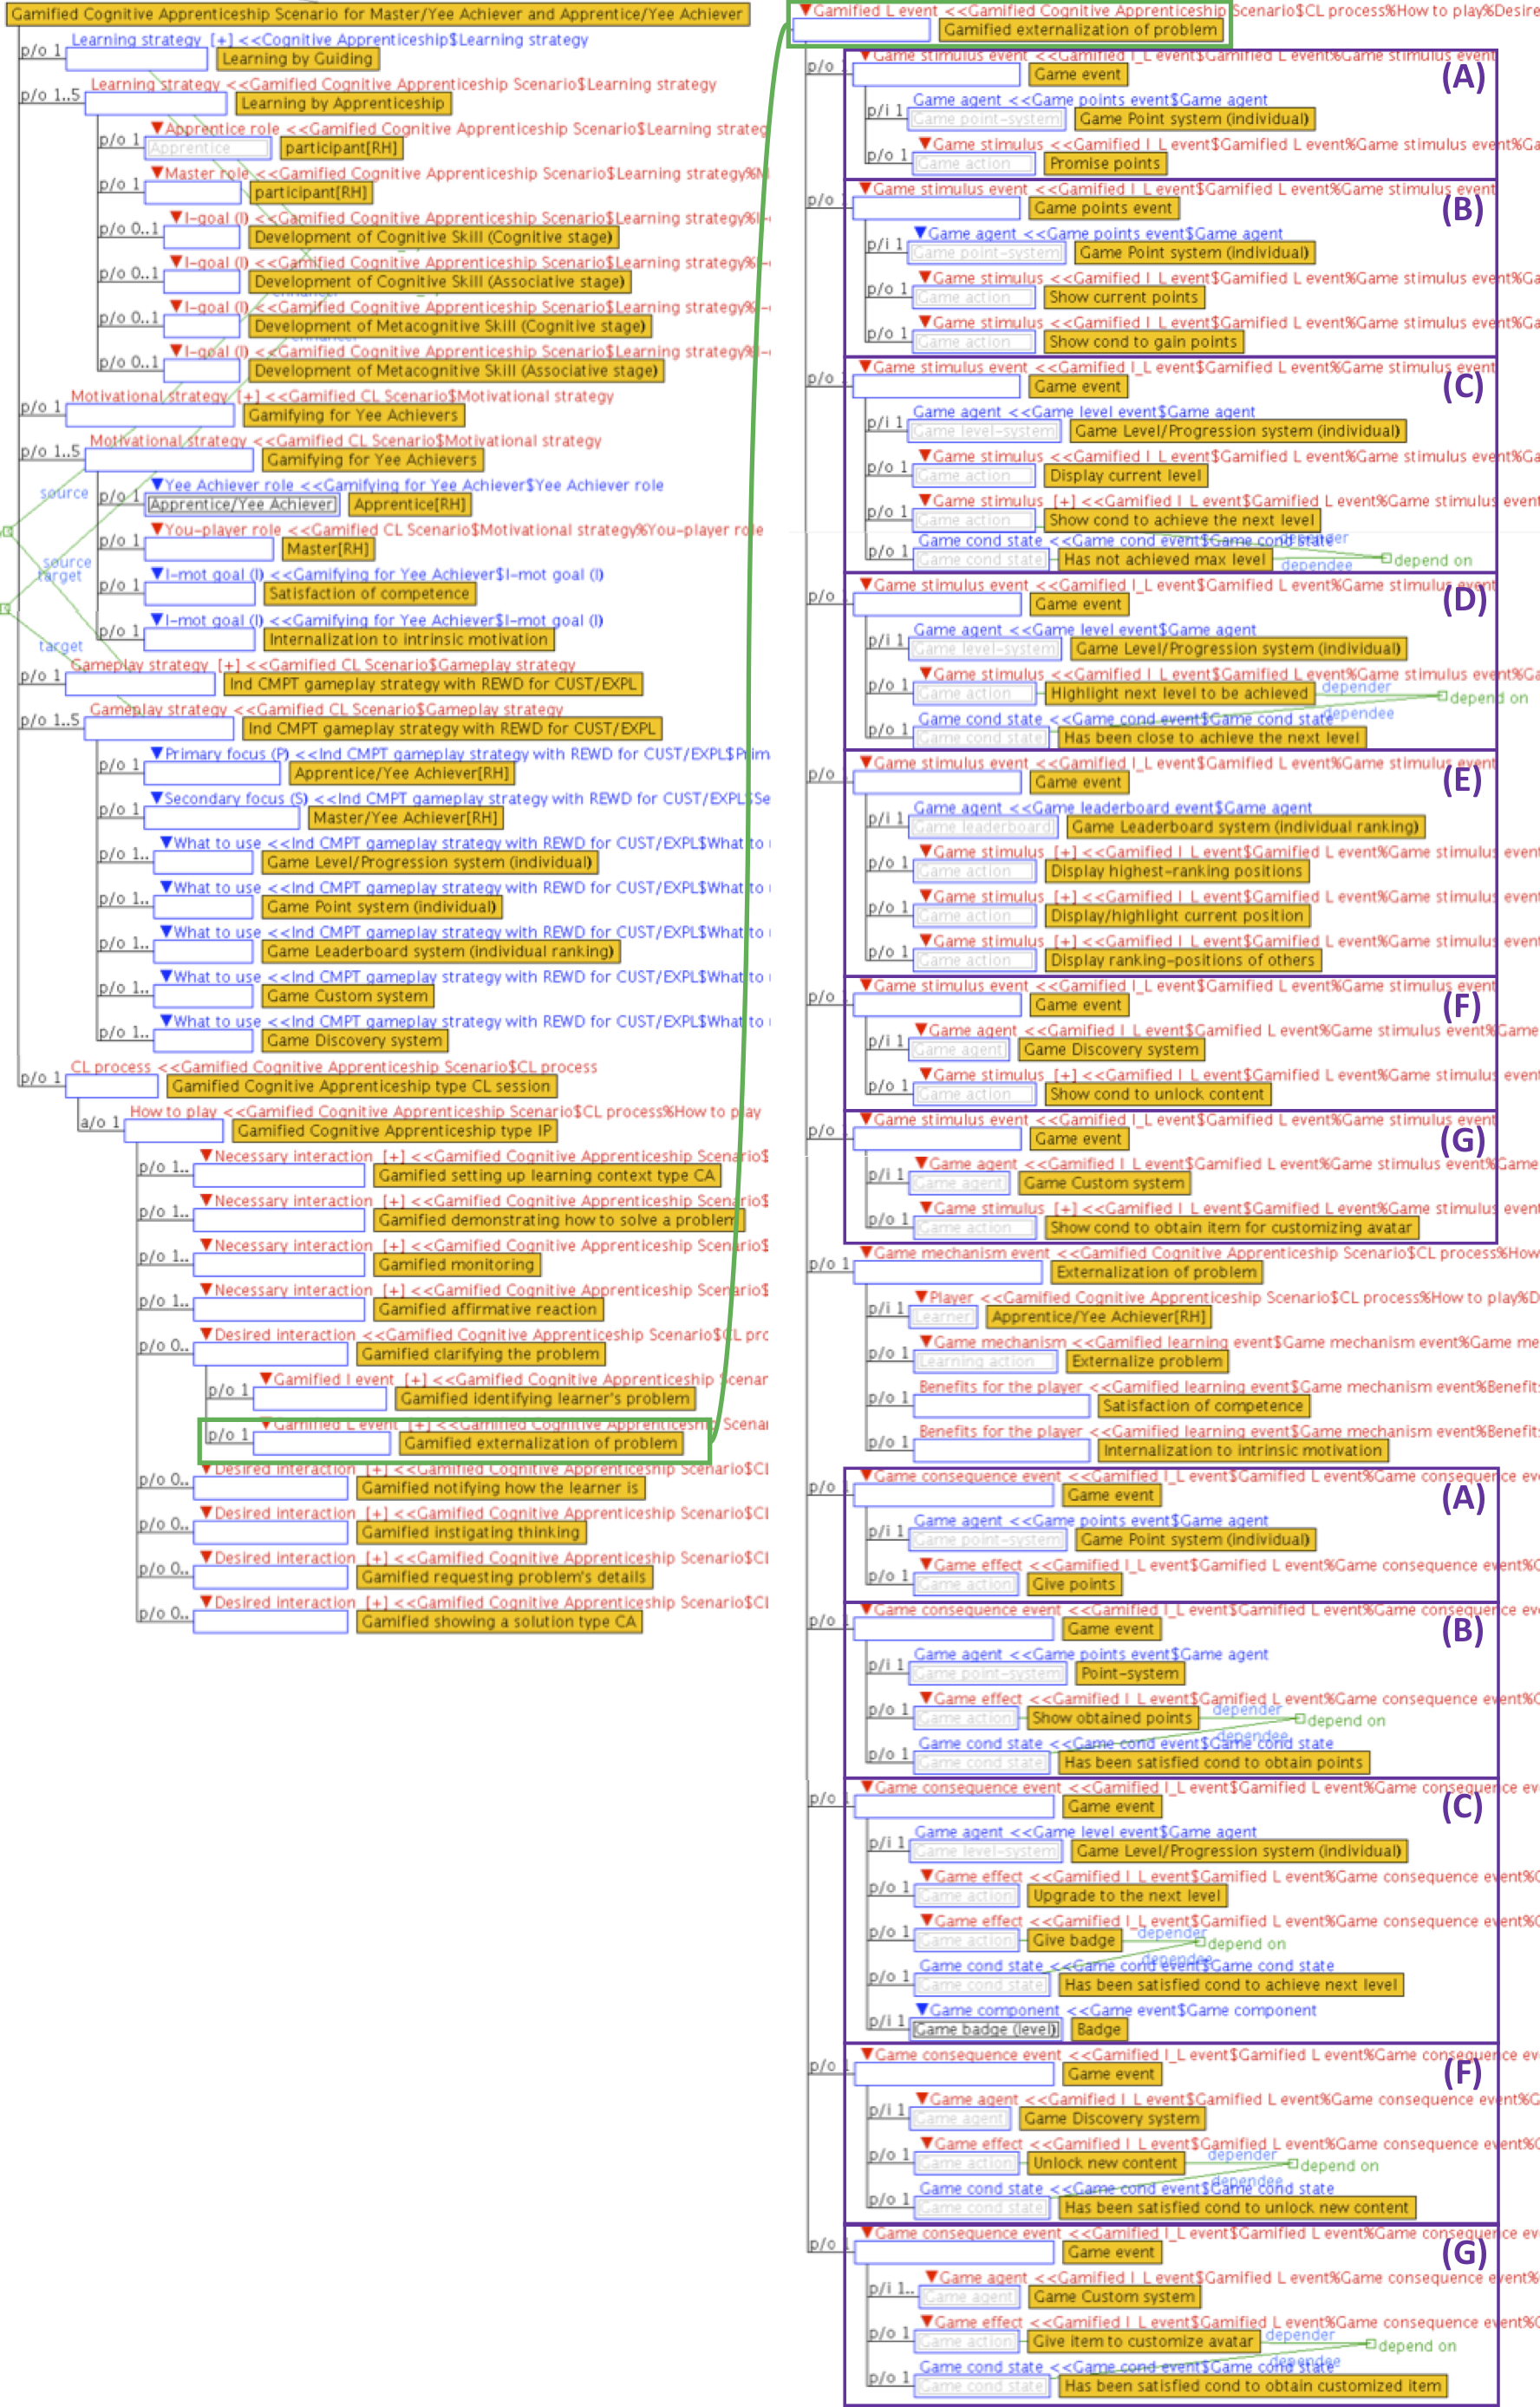
\includegraphics[width=0.95\textwidth]{images/chap-ontogacles2/ontological-structure-cognitive-apprenticeship-master-achiever-apprentice-achiever.png}
 \fautor
\end{figure}
\newpage

%%%%

On the right side of \autoref{fig:ontological-structure-cognitive-apprenticeship-master-achiever-apprentice-achiever} is detailed the gamified learning event \aspas{\emph{Gamified externalization of problem}} that is result of applying the combination of PGDSs \aspas{\emph{SEMT/SUGG, CMPT/CMPR, COOP, PERS, SIM, REWD, CUST}} to gamify the learning event \aspas{\emph{Externalization of problem}.} The application of the PGDS \aspas{\emph{Reward strategy based on PDS}} in the game element \aspas{\emph{Game Point system (individual)}} defined the game stimulus and consequence events indicated by the frames (A). According to these events, the game action defined as game stimulus is \aspas{\emph{Promise points},} and the game action defined as game effect is: \aspas{\emph{Give points}.} By applying the PGDSs \aspas{\emph{Self-monitoring strategy based on PDS}} and \aspas{\emph{Suggestion strategy based on the PDS}} in the game element \aspas{\emph{Game Point system (individual)},} the game stimulus and consequence events indicated in the frames (B) were obtained, where the game actions \aspas{\emph{Show current points}} and \aspas{\emph{Show cond to gain points}} are game stimulus, and the game action \aspas{\emph{Show obtained points}} is a game effect. The game actions \aspas{\emph{Display current level}} and \aspas{\emph{Show cond to achieve the next level}} as game stimulus, and the game action \aspas{\emph{Upgrade to the next level}} as game effect were result of applying the PGDSs \aspas{\emph{Self-monitoring strategy based on PDS}} and \aspas{\emph{Suggestion strategy based on the PDS}} in the game element \aspas{\emph{Game Level/Progression system (individual)}}. These game stimulus and game effects formalized as game events are shown in the frames (C). By applying the PGDS \aspas{\emph{Simulation strategy based on the PDS}} in the game element \aspas{\emph{Game Level/Progression system (individual)},} the game stimulus event shown in the frame (D) has been formalized as the game action \aspas{\emph{Highlight next level to be achieved}} when a participant \emph{Has been close to achieve the next level}. The game stimulus event shown in the frame (E) with the game actions \aspas{\emph{Display highest-ranking positions},} \aspas{\emph{Display/highlight current position}} and \aspas{\emph{Display ranking-positions of others}} has been obtained by the application of PGDSs \aspas{\emph{Competition strategy based on the PDS}} and \aspas{\emph{Comparison strategy based on the PDS}} in the game element \aspas{\emph{Game Leaderboard system (individual ranking)}.} The application of the PGDS \aspas{\emph{Personalization strategy based on PDS}} in the game element \aspas{\emph{Game Custom system}} defined the game stimulus and consequence events shown in the frames (F), where the game action \aspas{\emph{Show cond to unlock content}} is defined as a game stimulus, and where the game action \aspas{\emph{Unlock new content}} is defined as game effect. Finally, the game stimulus and consequence events shown in the frame (G) has been obtained by the application of the PGDS \aspas{\emph{Customization strategy based on PDS}} in the game element \aspas{\emph{Game Discovery system},} where the game action \aspas{\emph{Show cond to obtain item for customizing avatar}} is a game stimulus, and the game action \aspas{\emph{Give item to customize avatar}} is a game effect.

\subsubsection*{Step (3): Defining the game states and game components in the CL Game dynamic to provide a gameplay experience according to the individual gameplay strategies}
 
The last step in the formalization of ontological models to apply gamification as persuasive technology consists in the definition of game states and game components in the CL Game dynamic to connect the selected game elements. This connection is also established by setting of the game action in the game stimulus and consequence events. To engender a gameplay experience of individual competition for the Master/Yee Achiever role holders in the \aspas{\emph{Gamified Cognitive Apprenticeship Scenario for Master/Yee Achiever and Apprentice/Yee Achiever},} the \emph{Game Level/Progression system (individual)} is connected to the \emph{Game Point system (individual)} by setting of the condition to achieve the next level in the game action \aspas{\emph{Show cond to achieve the next level}} as shown in \autoref{fig:ontological-structures-connection-gameplay-experience} (A), where the condition \aspas{\emph{Has obtained [n] individual game points}} is defined as a state to be achieved by the \emph{Apprentice/Yee Achiever role holder} (\emph{owner}) \emph{from} a \emph{Game Point system (individual)}. The game element \aspas{\emph{Game Leaderboard system (individual ranking)}} is connected to the \aspas{\emph{Game Point system (individual)}} to define individual rankings based on the individual points as shown in \autoref{fig:ontological-structures-connection-gameplay-experience} (B).

\begin{figure}[!htbp]
 \caption[Connection of game elements to establish a gameplay experience of individual competition in the \emph{Gamified Cognitive Apprenticeship Scenario for Master/Yee Achiever and Apprentice/Yee Achiever}]{Connection of game elements to establish a gameplay experience of individual competition in the \aspas{\emph{Gamified Cognitive Apprenticeship Scenario for Master/Yee Achiever and Apprentice/Yee Achiever}.}}
 \label{fig:ontological-structures-connection-gameplay-experience}
 \centering
 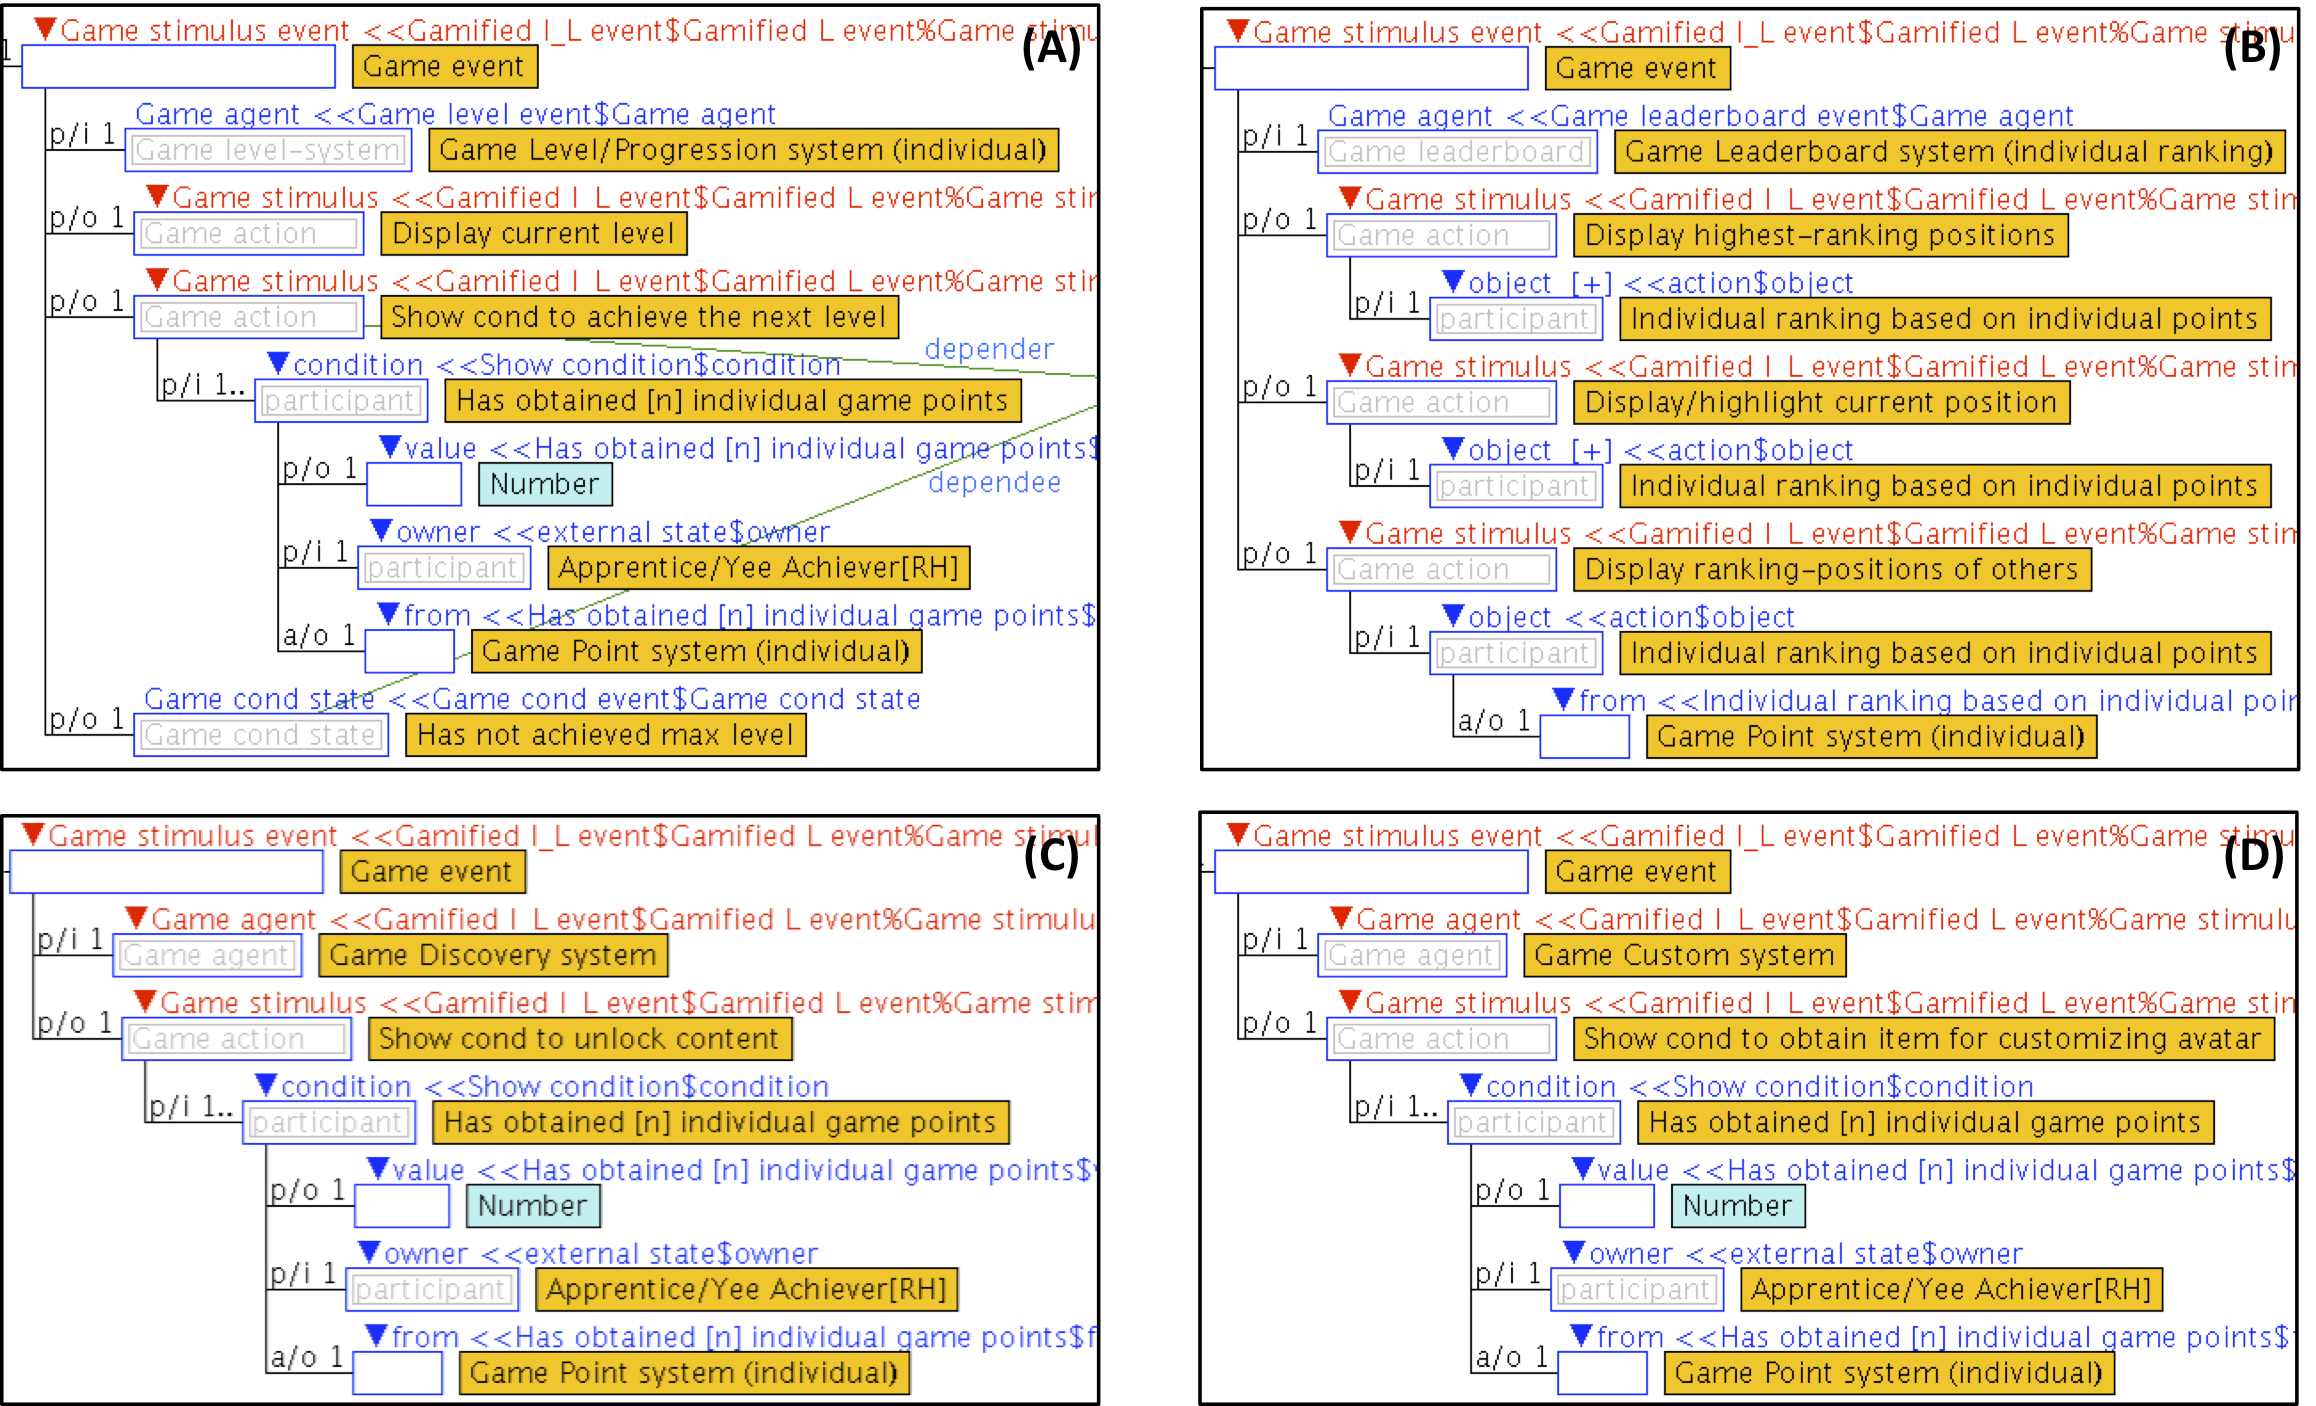
\includegraphics[width=0.95\textwidth]{images/chap-ontogacles2/ontological-structures-connection-gameplay-experience.png}
 \fautor
\end{figure}

\autoref{fig:ontological-structures-connection-gameplay-experience} (C) shows the setting for the connection between the game elements \aspas{\emph{Game Point system (individual)}} and \aspas{\emph{Game Discovery system}} in which the condition \aspas{\emph{Has obtained [n] individual game points}} for the game stimulus \aspas{\emph{Show cond to unlock content}} is established as the state own by the \emph{Apprentice/Yee Achiever role holder} (\emph{owner}) given \emph{from} the \emph{Game Point system (individual)}. This connection is defined to unlock new content in the system when the master achiever role holder gained [n] points. The configuration to give items for customizing avatar is show in \autoref{fig:ontological-structures-connection-gameplay-experience} (D), where the condition to perform the game action \aspas{\emph{Show cond to obtain item for customizing avatar}} is that the apprentice achiever role holder \aspas{\emph{Has obtained [n] individual game points}.} Thus, the attribute-of (\emph{a/o}) \aspas{\emph{from}} has been defined as \emph{Game Point system (individual)}, and the owner role is played by the \aspas{\emph{Apprentice/Yee Achiever[RH]}.}

%%%%%%%%%%%%%%%%%%%%%%%%%%%%%%%%%%%%%%%%%%%%%%%%%%
\section{Concluding Remarks}
\label{sec:ontogacles2-concluding-remarks} 

Gamification as persuasive technology has been formalized in this chapter as the application of Persuasive Game Design Strategies (PGDSs) in non-game events to gamify them. Thus, to represent the knowledge involved in this process as ontological structures, the author of this thesis has proposed a nested structure of non-game world, game world and gamification world to identify, classify and differentiate the elements related to non-game events and game events. With this classification, the link between the Persuasive Game Design (PGD) and the design of CL process is represented in explicitly form by \emph{gameplay events}. The prescriptive representation of the link between PGD and the design of CL process has been formalized by means of \emph{WAY-knowledge of PGDS}. This formalization is accomplished through the representation of \aspas{\emph{What}} and \aspas{\emph{How}} to achieve expected changes in person's attitudes, intentions, motivations and/or behaviors to persuade him/her to perform the actions specified in the non-game events. The design rationale in the application of PGDs to gamify a non-game event has been formalized as the concept of \aspas{\emph{Gameplay Scenario Model},} and it is used to gamify instructional and learning events defined in interactions patterns based on the sequencing mechanism of a CSCL script. Thus, the pairs of gamified instructional and learning events has been formalized as ontological structures under the concept of \emph{Gamified I\_L event} to represent an interaction in the CL process. As result of the application of PGDSs in the interaction pattern, a \emph{CL Game dynamic} is obtained to establish a \emph{CL Gameplay} in a gamified CL scenario. 

The usefulness of the ontological structures proposed here has been demonstrated by the formalization of an ontological model to apply gamification as persuasive technology in gamified CL scenarios based on the Cognitive Apprenticeship theory and with the player roles based on the Yee's model. The application of PGDSs to apply gamification as persuasive technology has the purpose to engender gameplay experiences of individual and cooperative competition based on the information extracted from the Model-driven persuasive game proposed by \citeonline{Orji2014}. 

To solve the context-dependency of gamification in CL scenarios to persuade the participants to follow the interactions defined by the sequencing mechanism of a CSCL script, computer-based mechanisms can be built to help the design of CL gameplay in gamified CL scenarios. This support is given by information extracted from ontological models to apply gamification as persuasive technology in which the ontological structures to represent gamified I\_L events are used to establish the interactions between participants and game elements in the environment to run the gamified CL scenarios. Employing the formalization of WAY-knowledge of PGDS, computer-based mechanisms that support the building of a WAY-knowledge base of PGDSs can be built and computer-based mechanism that support the building of ontological models to apply gamification as persuasive technology in gamified CL scenarios. These computer based mechanism will be presented in \autoref{chapter:computer-based-mechanisms-procedures}. 
